\documentclass[master=emnan,masteroption=ne]{kulemt}
\usepackage{subfig}
\usepackage{xfrac}
\usepackage{mathtools}
\setup{% Remove the "%" on the next line when using UTF-8 character encoding
  inputenc=utf8,
  title={Tuning Threshold Voltage in Organic Electrochemical Transistors by Varying Doping of the Conjugated Polymer p(g3T2-T)},
  author={Marielena Velasco Enriquez},
  promotor={Prof.\,Dr.\,Karl Leo\and Prof. Dr. Steven De Feyter},
  assessor={PD Dr.rer.nat.habil. Hans Kleemann},
  assistant={MSc. Anton Weissbach}}
% Remove the "%" on the next line for generating the cover page
%\setup{coverpageonly}
% Remove the "%" before the next "\setup" to generate only the first pages
% (e.g., if you are a Word user).
%\setup{frontpagesonly}

% Choose the main text font (e.g., Latin Modern)
\setup{font=lm}

% If you want to include other LaTeX packages, do it here. 

% Finally the hyperref package is used for pdf files.
% This can be commented out for printed versions.
%\usepackage[pdfusetitle,colorlinks,plainpages=false]{hyperref}
\usepackage[pdfusetitle,hidelinks,plainpages=false]{hyperref}

%%%%%%%
% The lipsum package is used to generate random text.
% You never need this in a real master's thesis text!
\IfFileExists{lipsum.sty}%
 {\usepackage{lipsum}}%
 {\newcommand{\lipsum}[1][1-7]{\par And some text: lipsum ##1.\par}}
%%%%%%%

%\includeonly{chap-n}
\begin{document}

\begin{preface}
  %I would like to thank everybody who kept me busy the last year, especially my promoter and my assistants. I would also like to thank the jury for reading the text. My sincere gratitude also goes to my wive and the rest of my family.
\end{preface}

\tableofcontents*

\begin{abstract}
Organic Electrochemical Transistors (OECTs) exhibit advantageous properties, such as high transconductance and steep-slope switching, while operating at very low voltages. Although, their switching speed is comparatively slower than solid-state devices, it remains sufficient for applications in bioelectronics \cite{rivnayOrganicElectrochemicalTransistors2018}. The gold standard conjugated polymer for p-type OECTs is PEDOT:PSS. However, its main drawback lies in its depletion-mode operation, which requires power to turn off the device. To minimize power consumption and improve stability, efforts have been made to the design conjugated polymers that allow accumulation-mode devices. One such polymer, 3-(2-(2-(2-methoxyethoxy)ethoxy)ethoxy)thiophene (p(g3T2-T)) has demonstrated negative threshold voltages close to zero and high transconductance \cite{nielsenMolecularDesignSemiconducting2016}. Furthermore, by doping p(g3T2-T) at various levels and drop-casting it as a gate, it has been possible to fine-tune the threshold voltage \cite{tanTuningOrganicElectrochemical2022}. This study aims to adapt a microstructuring method for fabricating side-gated OECT devices that comprises different doping levels of F$_{4}$TCNQ and F$_{6}$TCNNQ in p(g3T2-T) and a solid-state electrolyte \cite{weissbachPhotopatternableSolidElectrolyte2022}, the latter is deposited by inkjet printing. Additionally, the study aims to adjust the threshold voltage by utilizing these varying doping levels, while analyzing the stability and performance of the doped devices.

  %\lipsum[1]
\end{abstract}

% A list of figures and tables is optional
\listoffigures
\listoftables
% If you only have a few figures and tables you can use the following instead
%\listoffiguresandtables
% The list of symbols is also optional.
% This list must be created manually, e.g., as follows:
%\chapter{List of Abbreviations and Symbols}
%\section*{Abbreviations}
%\begin{flushleft}
%  \renewcommand{\arraystretch}{1.1}
%  \begin{tabularx}{\textwidth}{@{}p{12mm}X@{}}
%    OECT   & Organic Electrochemical Transistor \\
%    Vth   & Threshold Voltage \\
%    CV  & Cyclic Voltammetry \\
%    EIS  & Electrical Impedance Spectroscopy \\
%    UPS  & Ultraviolate Photoelectron Spectroscopy \\
%    XPS  & X-Ray Photoelectron Spectroscopy \\
%  \end{tabularx}
%\end{flushleft}
%\section*{Symbols}
%\begin{flushleft}
%  \renewcommand{\arraystretch}{1.1}
%  \begin{tabularx}{\textwidth}{@{}p{12mm}X@{}}
%    $c$   & Speed of light \\
%    $E$   & Energy \\
%    $m$   & Mass \\
%    $\pi$ & The number pi \\
%  \end{tabularx}
%\end{flushleft}

% Now comes the main text
\mainmatter

\chapter{Introduction}
\label{cha:intro}

The field of organic electronics has witnessed significant advancements in recent years due to its biocompatibility, mechanical compliant, and other application-specific characteristics. Among the numerous types of organic devices, Organic Electrochemical Transistors (OECTs) have attracted considerable attention due to their unique capabilities such as high transconductance and steep-slope switching at low operation voltages, which give them potential for use in energy storage, bioelectronics and neuromorphic devices. 

Accumulation-mode transistors, devices that are normally in the OFF state at zero-gate-biased condition, rely on the use of undoped conjugated polymers. In constrast, the ability to precisely control and tune threshold voltage of an OECT can be achieve by manipulating the doping level of the mentioned conjugated polymer \cite{tanTuningOrganicElectrochemical2022}. Tan et al. fabricated devices that did not follow a complete microstructuring technique, limiting their integration into circuits. 

%\section{Motivation}
%Many challenges have raised for OECTs' operation, some of them include and will be the main focus of this thesis:
%\begin{itemize}
%\item The fabrication of accumulation-mode transistors, devices that are normally in the OFF state at zero-gate-biased condition.
%\item The modulation of their threshold voltage that allow the integration to different circuit designs.
%\end{itemize}

%\section{Goal}
%Understanding the relationship between the doping level and threshold voltage shift is crucial for the design and fabrication of high performance OECTs

The primary objective of this research is to address this missing information by developing a microstructuring method to fabricate accumulation-mode OECTs with controlled doping levels and enable their seamless integration into circuits. However, during the pursuit of this objective, it was identified that stability of dopants in an electrochemical environment may pose challenges that need to be addressed as well. Therefore, this research project specifically aims to:

\begin{enumerate}
\item Characterize 3-(2-(2-(2-methoxyethoxy)ethoxy)ethoxy)thiophene (p(g3T2-T)) with varying doping levels of F$_{4}$TCNQ and F$_{6}$TCNNQ. This involves chemically modifying the conjugated polymer with different concentrations of dopant and analyzing their electronic structure, morphology and electrical properties using techniques such as UV-Vis spectroscopy, Ultraviolet Photoelectron Spectroscopy (UPS), Atomic Force Microscopy (AFM), Van Der Pauw method, Electrical Impedance Spectroscopy (EIS) and Cyclic Voltammetry (CV),

\item fabricate OECT devices, which involves utilizing the conjugated polymer at different doping levels, and adapting an existing method that combines electrode patterning techniques, spin-coating, photolithography and inkjet printing. The devices will be carefully optimized to ensure reproducibility and stability,
 
\item assess doped polymer stability in OECT, which involves performing conductivity measurements over time and selecting an electrolyte composition that allows an stable performance, and
 
\item investigate the shift in threshold voltage through electrical characterization of the fabricated OECT devices with varying doping levels of F$_{4}$TCNQ and F$_{6}$TCNNQ.


\end{enumerate}

%\section{Structure of the Work}
The thesis is structured as follows: Chapter 1 provides an overview of organic electronics and the importance of the OECT threshold voltage, and outlines the motivation, goals, and structure of the thesis. Chapter 2 presents a comprehensive review of the relevant background information on Organic Semiconductors (OSCs), Organic Mixed Ionic Electronic Conductors (OMIECs), and Organic Electrochemical Transistors, and relevant research on tuning the threshold voltage of OECTs. Chapter 3 illustrates the Experimental Methods used in this research, describes the materials, equipment, software, and procedures to chemically doped the films and characterization method employed in the study. Finally, it outlines the fabrication and characterization process of OECT devices. In Chapter 4, the experimental results obtained are presented, from the characterization of the conjugated polymer at different doping levels and fabricated OECT devices. Analysis of the relationship between the doping level and the shift in threshold voltage. Finally, it discusses the implications of the findings and their relevance to the field. Lastly, Chapter 5 provides a summary of the research objectives and the extent to which they were achieved, suggests future research direction, and potential applications.

By addressing the aforementioned research goals and following the proposed thesis structure, this study aims to contribute in adapting an existing protocol to the conjugated material p(g3T2-T), in understanding the doping-dependent tuning of OECT threshold voltage and establish a foundation for the development of high-performance organic electronic devices.

%%% Local Variables: 
%%% mode: latex
%%% TeX-master: "thesis"
%%% End: 

\chapter{Background} \label{chap:background}

\section{Organic Semiconductors}

%When atoms bond together, molecular orbital are defined by the linear combination of atomic orbitals, however the symmetry shown on some complex structures are not explained by a simple linear combination, instead hybrid atomic orbitals are formed. This mathematical process is called \textbf{hybridization}.
Unlike inorganic semiconductors, organic semiconductors are lightweight, easy to chemically tune, mechanically flexible, and offer low-cost and low-temperature processing. All of these characteristics are responsible for the increased attention to this type of material in the field of organic electronics. 

%\subsection{Conjugated polymers}
%\subsection{Small molecules}

\subsection{Electronic Structure and Transport} 

Organic semiconductors are $\pi$-conjugated molecules that comprise mostly carbon and hydrogen atoms, with alternating multiple (sp$^{2}$ hybridization) and single (sp hybridization) bonds. The wavefunction of the sp$^{2}$ orbitals overlap so that electrons are delocalized.
%This configuration exhibit $p$-orbitals with delocalized electrons. %, charge transport among the length of these polymers is caused by the alternation of these bonds, describing a resonance structure. 
Based on the size of the conjugated system, organic semiconductors can be divided into conjugated polymers and small molecules. The latter have the advantage that their synthesis and low molecular mass allows to obtain them high purity material \cite{alcacerElectronicStructureOrganic2018}.
% of being ordered and its synthesis allows to obtain high purity material \cite{alcacerElectronicStructureOrganic2018}.

\begin{figure}[ht]
  \centering
  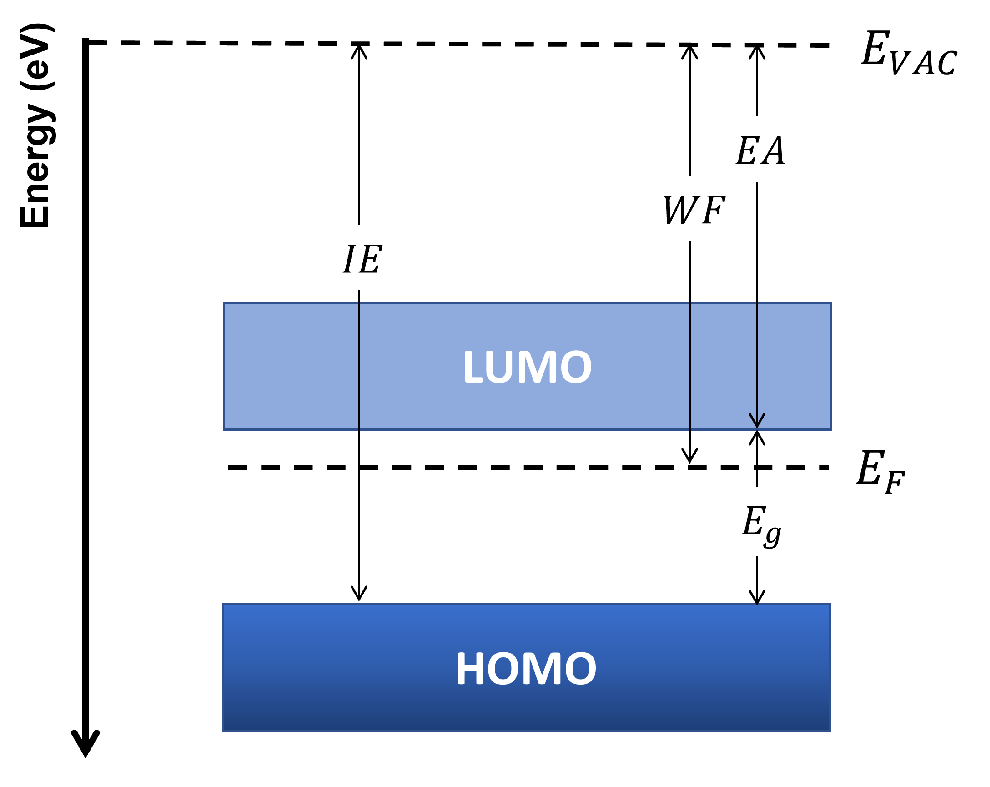
\includegraphics[width=6cm]{Images/pdf/ediagram.pdf}
  \caption[Energy level diagram of organic semiconductors]{Energy level diagram of an p-type doped organic semiconductor.}
  \label{fig:ediag}
\end{figure}

The energy structure of organic semiconductors comprises a highest occupied molecular orbital (HOMO) state and a lowest unoccupied molecular orbital (LUMO) state, which are analogous to the valence and conduction bands, respectively, from inorganic semiconductors. The difference between these energy levels corresponds to the energy gap (E$_{g}$) of the material, as illustrated in Figure \ref{fig:ediag}. Additionally, we can define i) the Fermi level (E$_{F}$) using the material's work function (WF), ii) the ionization energy (IE), also referred as ionization potential (IP), using the HOMO energy, and iii) the electron affinity (EA), using the LUMO energy.

%\subsubsection{Conjugated polymers}
%Semiconducting properties of conjugated polymers built by alternating electron donor and acceptor moieties \cite{mattElectronicStructureMorphology2021}, 
%Since inorganic semiconductors' band models does not take into consideration the Coulomb and exchange electron-electron interaction, which play a major role in organic semiconductors, it is necessary to add new theoretical approaches. On one hand, the transport properties are better described in terms of a hopping mechanism and the optoelectronic properties are better described by the molecular orbital picture \cite{alcacerElectronicStructureOrganic2018}. Since the device under study in this work is a transistor and their transport properties in aqueous and quasi-solid environments, the theoretical approach used will be the hopping mechanism.

%Transport properties depend on the details of the band structure, namely the density of states and the band widths

%\subsubsection{Small Molecules}
%Unlike conjugated polymers, the chain size of small molecules have the advantage of being ordered and its synthesis allow to obtain high purity material.

%\subsection{Electronic Transport}

Organic semiconductor materials can also be classified based on whether their ground state is degenerate or non-degenerate. In the former case, the term ``degenerate'' describes monomers that have equivalent energy states in the ground state. In contrast, in the latter case, the ground state exhibits non-degeneracy, which is commonly observed due to the energy difference of aromatic (benzoid) and quinoid structures \cite{heegerSolitonsConductingPolymers1988a}, as exhibited in Figure \ref{fig:energy}.

\begin{figure}[ht]
  \centering
  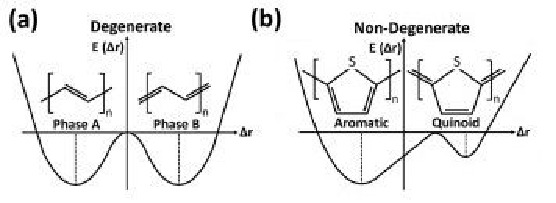
\includegraphics[width=12cm]{Images/pdf/deg_pol.pdf}
  \caption[Degenerate and non-degenerate conjugated polymers]{Potential energy change (electronic plus lattice distortion energy) in A) degenerate and B) non-degenerate ground-state-conjugated polymers. Extracted from reference \cite{heydarigharahcheshmehTextureNanostructuralEngineering2020}.}
  \label{fig:energy}
\end{figure}

%Transport in an organic semiconductor creates changes in the bond-length alternation pattern. Since charge transport come together with a chain distortion, new quasiparticles are defined: solitons in degenerate molecules and polarons in non-degenerate molecules \cite{bredasRoleMobileOrganic1984}.
In electronic transport theory for organic semiconductors, the concept of polarons is introduced. This quasiparticle effectively captures the alteration of the bond-length alternation pattern induced by the movement of charge carriers (electrons or holes) \cite{bredasRoleMobileOrganic1984}. This alteration can be observed, for instance, when transitioning from Phase A to Phase B in degenerate molecules, or from aromatic to a quinoid structure in non-degenerate molecules.

 %Since charge transport come together with a chain distortion, new quasiparticles are defined in transport theory, in a degenerated molecule, the quasiparticles are named solitons, and in a non-degenerated molecule, a bound soliton-antisoliton is formed in the benzoid structures, the pair receive the name of polaron. This pair annihilate in the quinoid structure in between forming a double bond so neutral polarons are not stable \cite{bredasRoleMobileOrganic1984}.

\subsection{Molecular Doping} \label{subsec:moldop}
The basic principles of molecular doping are similar than in inorganic materials. A donor or acceptor entity is added to generate electrons or holes, as shown in Figure \ref{fig:dopscheme}. While n-type dopants donate electrons to the LUMO state, the p-type dopants extract electrons from the HOMO state, thus creating holes \cite{lussemDopingOrganicSemiconductors2013}. In other words, the Fermi level E$_{F}$ of the polymer will shift towards the LUMO (or HOMO) level when there is n-type (or p-type) doping. This shift can be quantified using spectroscopy techniques such as Ultraviolet Photoelectron Spectroscopy (UPS) \cite{tietzeFermiLevelShift2012}, although it may be somewhat limited by the penetration depth of the exciting electrons.

\begin{figure}[ht]
  \centering
  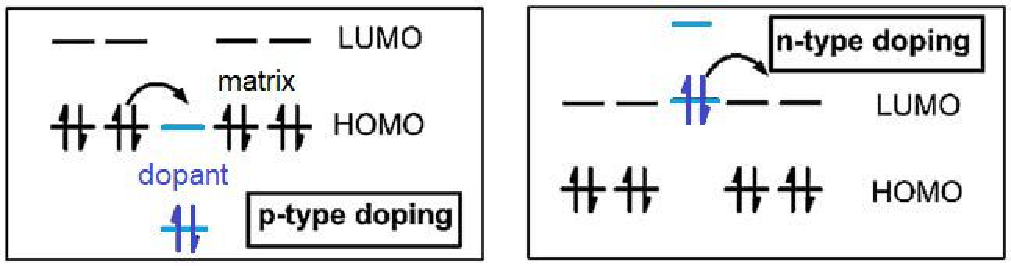
\includegraphics[width=12cm]{Images/pdf/doping.pdf}
  \caption[Scheme of doping processes in organic semiconductors]{Schemes for p-type (left) and n-type (right) doping processes.}
  \label{fig:dopscheme}
\end{figure}

When doping occurs, %charged solitons come as outcome in a degenerated molecules. In a non-degenerated, our main focus in this work, 
the formation of a new quasiparticle named bipolaron occurs. For instance, if p-type dopants are introduced to a degenerate molecule (as depicted in Figure \ref{fig:bipol}), electrons are removed from double bonds. Focusing on a single event, this removal leaves one carbon positively charged, with an adjacent carbon atom possessing an unpaired electron. This unpaired electron moves along the polymer chain until it encounters another unpaired electron from a separate doping event. When they come together, they form a double bond, resulting in the creation of two charged polarons: a bipolaron \cite{bredasPolaronsBipolaronsSolitons1985}. %Although, a nice simplification, in a degenerated molecule is not realistic, but usually

\begin{figure}[ht]
  \centering
  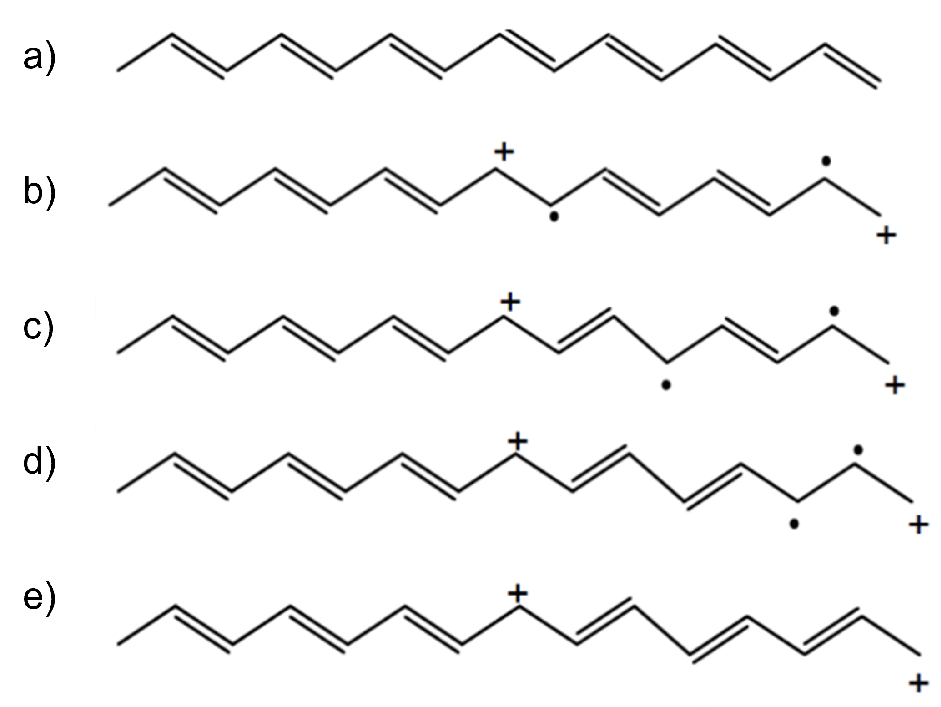
\includegraphics[width=10cm]{Images/pdf/bipolaron.pdf}
  \caption[Representation of bipolaron formation introduced via doping]{a) Structure of degenerate molecule. b) Electron extraction via doping. c) Unpaired electron shifting down. d) Unpaired electrons meet. e) Formation of double bond and two charged polarons: bipolaron.}
  \label{fig:bipol}
\end{figure}

The energy levels generated upon the formation of polarons and bipolarons in non-degenerate molecules are illustrated in Figure \ref{fig:ebipol}. As the doping density increases, the amount of bipolaron states also increases. Their overlapping leads to the formation of bipolaron bands, and the energy difference between the two in-gap states i and i*, as shown from Figure \ref{fig:ebipol}b to D, decreases. %Fix this part % \cite{bredasRoleMobileOrganic1984}

\begin{figure}[ht]
  \centering
  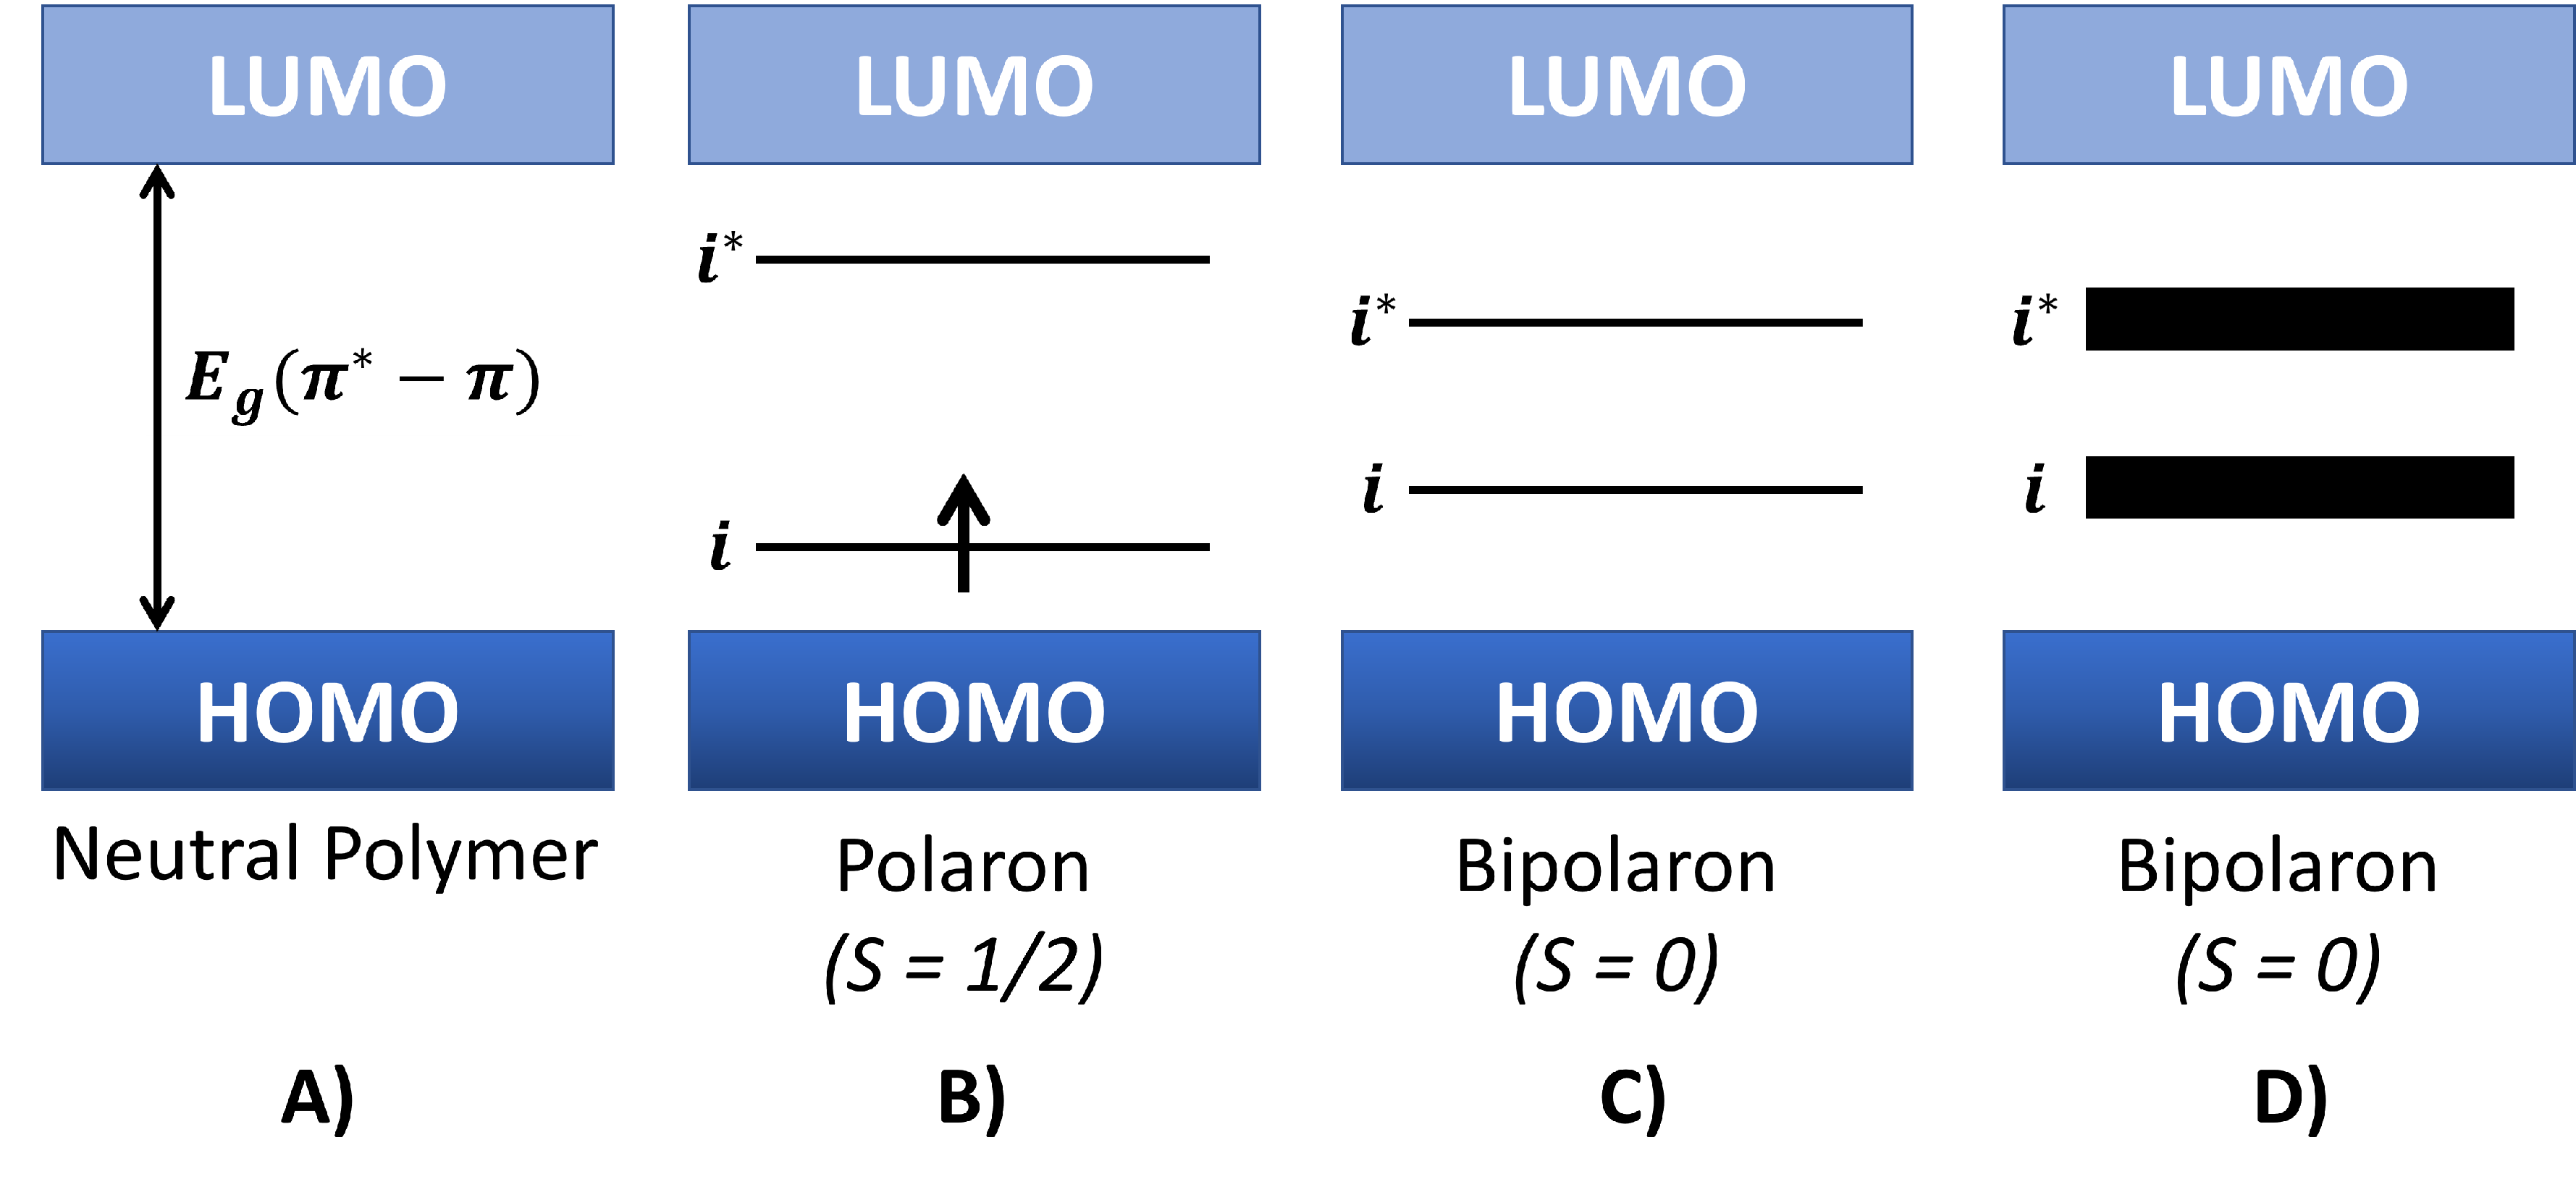
\includegraphics[width=10cm]{Images/pdf/bipolaron_bands.pdf}
  \caption[Formation of polaron, bipolaron, and bipolaron band]{Potential energy change of aromatic and quinoid in the non-degenerate ground-state A) neutral conjugated polymer, and formation of B) polaron, C) bipolaron, and D) bipolaron bands upon doping. Extracted from reference \cite{heydarigharahcheshmehTextureNanostructuralEngineering2020}.}
  \label{fig:ebipol}
\end{figure}

In addition to these new electronic states, the doped polymer will also exhibit distinct optical transitions that could be revealed through UV-Vis-NIR spectroscopy. In this technique, absorption peaks indicate the presence of these optical transitions. However, these transitions may not be precisely quantified or clearly defined \cite{heydarigharahcheshmehTextureNanostructuralEngineering2020}.
%Zozoulenko et al. proposed a new DFT-based description of the polaronic and bipolaronic states 
%% This specifics introduces to our graph

The use of small molecules as dopants for organic materials is commonly reported. Some strong acceptor (or electron-deficient) molecules that are widely used include 2,3,5,6 tetrafluoro-7,7,8,8-tetracyanoquinodimethane (F$_{4}$TCNQ) or 1,3,4,5,7,8 hexafluoro-7,7,8,8-tetracyanonaphthoquinodimethane (F$_{6}$TCNNQ), both of which are also relevant to this work. The latter exhibits a higher electronic affinity (-5.3 eV) than F$_{4}$TCNQ (-5.2eV), indicating that it can abstract electrons more efficiently, specially from polymers with low ionization potential (IP < 5eV) \cite{kieferDoubleDopingConjugated2019}%, as it is the case of p(g3T2-T) acting as donor
.

Among the various methods of molecular doping for conjugated polymers, Jacobs et al. conducted a comparison between solution-mixed and solution-sequential doping of P3HT, a thiophene-based polymer, doped with F$_{4}$TCNQ. These doping methods are considered straightforward and easy, especially when compared to other techniques such as vapor-phase doping \cite{fontanaEvaporationVsSolution2019}. Their research showed that solution-mixed films tend to have considerably rougher surface than solution-sequential films, which can negatively impact their conductivity \cite{jacobsComparisonSolutionmixedSequentially2016}. The fact that solution-sequential doped films exhibit better homogeneity also makes them more compatible with microstructuring processes such as photolithography. Reason why it is going to be used in this work and will be further detailed in Section \ref{subsec:films}. However, this advantage comes at the expense of having less control over the doping levels when compared to solution-mixed films \cite{tanOrganicMixedIonic2022}.

\section{Organic Mixed Ionic/Electronic Conductors (OMIECs)} \label{sec:omiecs}

Organic Mixed Ionic/Electronic conductors are a class of organic semiconductors that allow the conduction of electrons (or holes) and ions. This feature sets them apart from other organic semiconductors. %Organic semiconductors 
Commonly designed with polar side chains, OMIECs have been identified as a promising class of materials for the field of bioelectronics
%These materials, also called organic mixed ionic/electronic conductors (OMIECs), can exchange ions with aqueous electrolytes when electronic charge carriers are injected, transported, and stored in the bulk of the material
\cite{giovannittiEnergeticControlRedoxActive2020}. Initially investigated for batteries and super-capacitors \cite{snookConductingpolymerbasedSupercapacitorDevices2011}
\cite{liangOrganicElectrodeMaterials2012}, where the primary objective was to induce charges in a semiconducting polymer, OMIECs have rapidly expanded their scope to include other applications, among them, our focus: OECTs.
%Electronic charges accumulated on the conjugated polymer backbone result in secondary property changes in electrochemical potential and electronic conductivity \cite{tanOrganicMixedIonic2022}. 
% PEDOT:PSS Heterogeneous, blends or complexed systems OMIEC. Conjugated polymer/electrolyte blends. Contains ions chemically linked ot an insulating or conjugated component
% p(g3T2-T) Homogeneous, single-component systems OMIEC. Conjugated polymer electrolytes. Ions introduced as free species upon material casting or device operation
%change caption of figure

\begin{figure}[!htb]
  \centering
  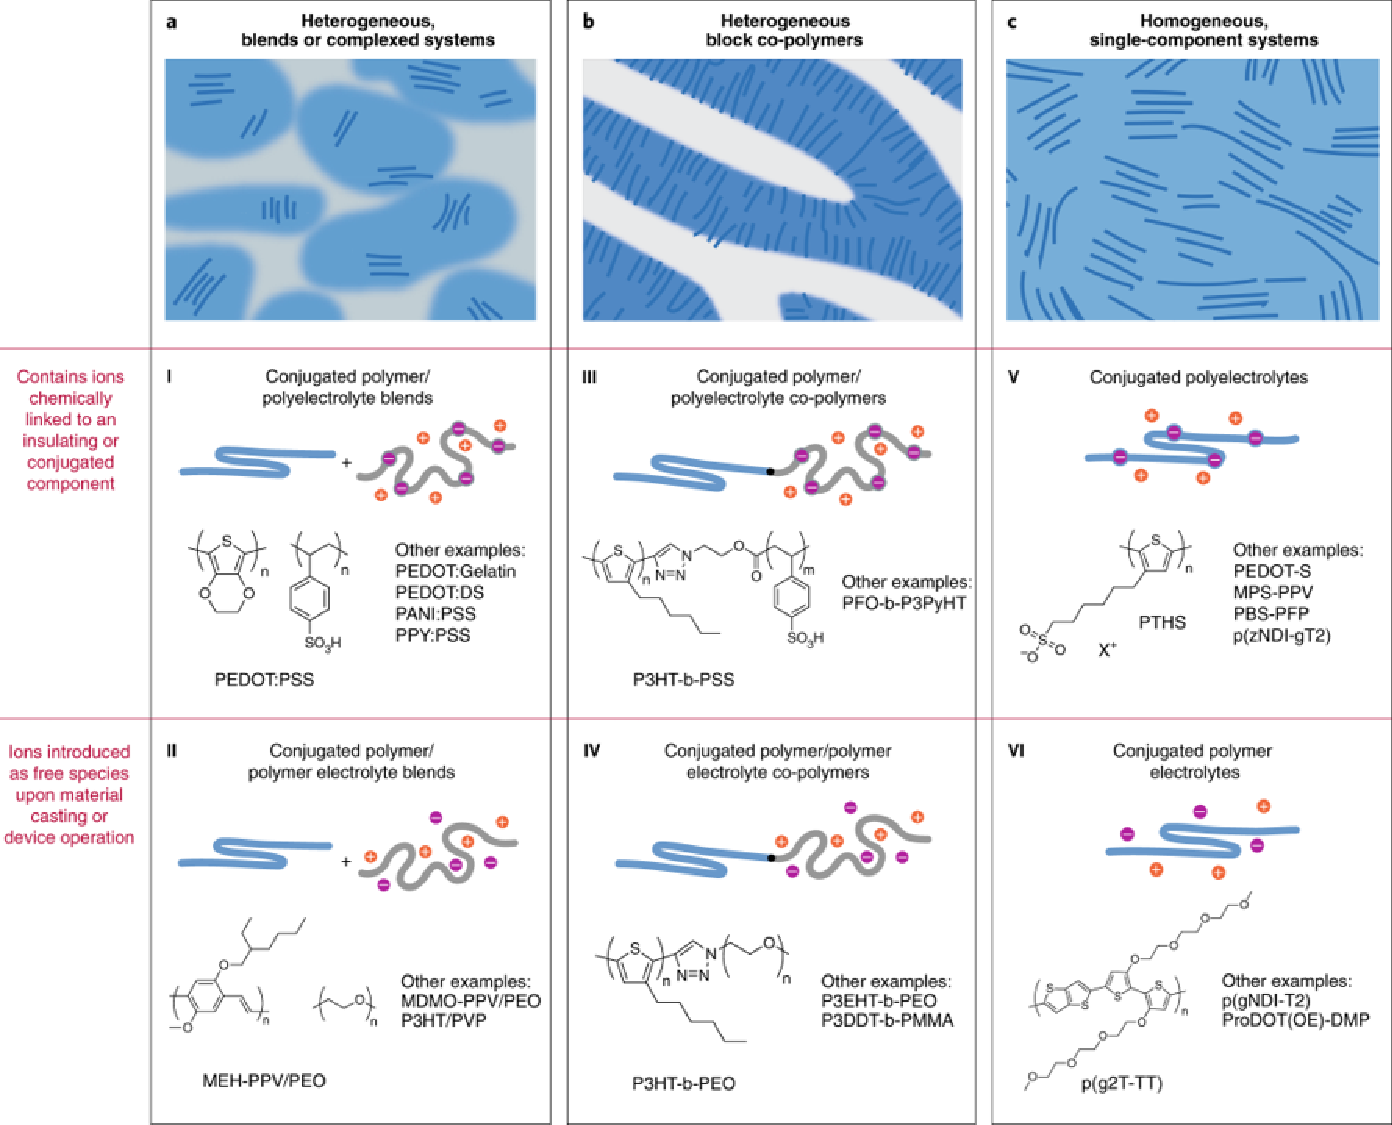
\includegraphics[width=\textwidth]{Images/pdf/OMIEC_types.pdf}
  \caption[Material classes of OMIECs]{\textbf{OMIECs classes.} a) Heterogeneous blends of a conducting conjugated polymer with (I) %an ionic charge bearing
  a polyelectrolyte or (II) an ion-solvating polymer electrolyte. %These systems frequently feature impure phases and can be largely disordered on multiple length scales. 
  b) Heterogeneous block copolymers of a conducting conjugated polymer with (III) %an ionic charge bearing
  a polyelectrolyte or (IV) an ion-solvating polymer electrolyte. %Such block copolymers often feature more well-defined pure phases and mesoscale order—readily synthetically tunable. 
  c) Fully conjugated (V) %ionic charge bearing
  polyelectrolytes and (VI) ion-solvating polymer electrolytes. %OMIEC types I–IV produce heterogeneous morphologies with microphase segregated predominately electron conducting and ion conducting domains. As shown in the sketches in the first row, in the case of blends (I and II) this occurs in a disordered fashion, or in the case of block copolymers (III and IV) it can occur in a variety of ordered structures (lamellar phase portrayed here). All-conjugated polyelectrolytes (V) and polymer electrolytes (VI) exist as a single mixed conducting phase that may contain heterogeneous composition of ordered and amorphous domains. Conceptual sketches (grey, ionic transport component; blue, electronic transport component; orange, cations; magenta, anions) 
  Extracted from reference \cite{paulsenOrganicMixedIonic2020}.}
  \label{fig:omiectypes}
\end{figure}

Paulsen et al. classified OMIECs into six different categories based on whether they \textit{``intrinsically contain ionic charge''} (I, III, V) or not (II, IV, VI), the latter group comprises materials that \textit{``contain polar moieties that can solvate ions''}. Another distinguishing factor among these categories is whether the conjugated system is composed of a single material (homogeneous, type V and VI) or a two-component, more complex systems or block co-polymer materials (heterogeneous, type I, II, III, IV)\cite{paulsenOrganicMixedIonic2020}. A schematic representation is shown in Figure \ref{fig:omiectypes}. %For instance, the conjugated polymer p(g3T2-T), used in this work, falls into a type VI OMIEC.


\subsection{Processes in OMIECs}

\subsubsection{Ionic-electronic interactions}
The presence of electronic charges in OMIECs %s in
requires also the presence of excess ionic charge, so charge in the system remains in balance. In the case of types II, IV, and VI OMIECs, a phenomenon known as stabilizing electrochemical doping is achieved through the presence of mobile ions that act as free charges. Conversely, other types of OMIECs have these stabilizing charges chemically bound and fixed, making them inherently doped.

% Explanation of parts where ion-coupling (electrostatic or direct electron transfer cases) occurs, and a third case where it does not occur, not necessary here, or would it be? I think this is the main difference on what is happening in my material, compared to PEDOT:PSS. So not sure if add the graphs

The degree of coupling between electronic charges and excess ionic charges in OMIECs can be modulated by applying a bias when connected through an electrolyte \cite{paulsenOrganicMixedIonic2020}. This fundamental principle forms the basis of OECTs, which will be discussed further in Section \ref{sec:OECTs}.

\subsubsection{Electronic transport}
%Electronic charge carrier density in undoped semiconductor organic species is logically low (no accessible hopping states), but in contact with an electrolyte, due to the ionic-electronic coupling as described in previous subsection, dopant ions would ... \cite{paulsenOrganicMixedIonic2020}. 

Electronic charge transport mechanisms present in OMIECs include thermally-activated hopping and band-like transport, as depicted in Figure \ref{fig:etrans}. These mechanisms are not different from those observed in other conjugated polymers. 

\begin{figure}[!htb]
	\centering
	\subfloat[\textbf{Thermally activated hopping}]{{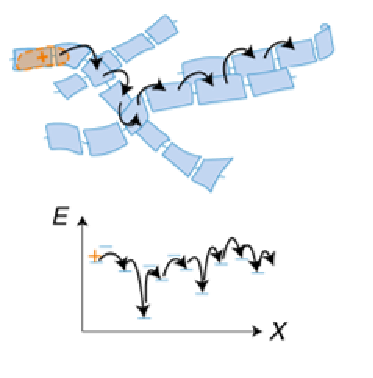
\includegraphics[width=5cm]{Images/pdf/OMIECetransport1.pdf} }}
	%\qquad
	\hspace{2em}
	\subfloat[\textbf{Band-like transport}]{{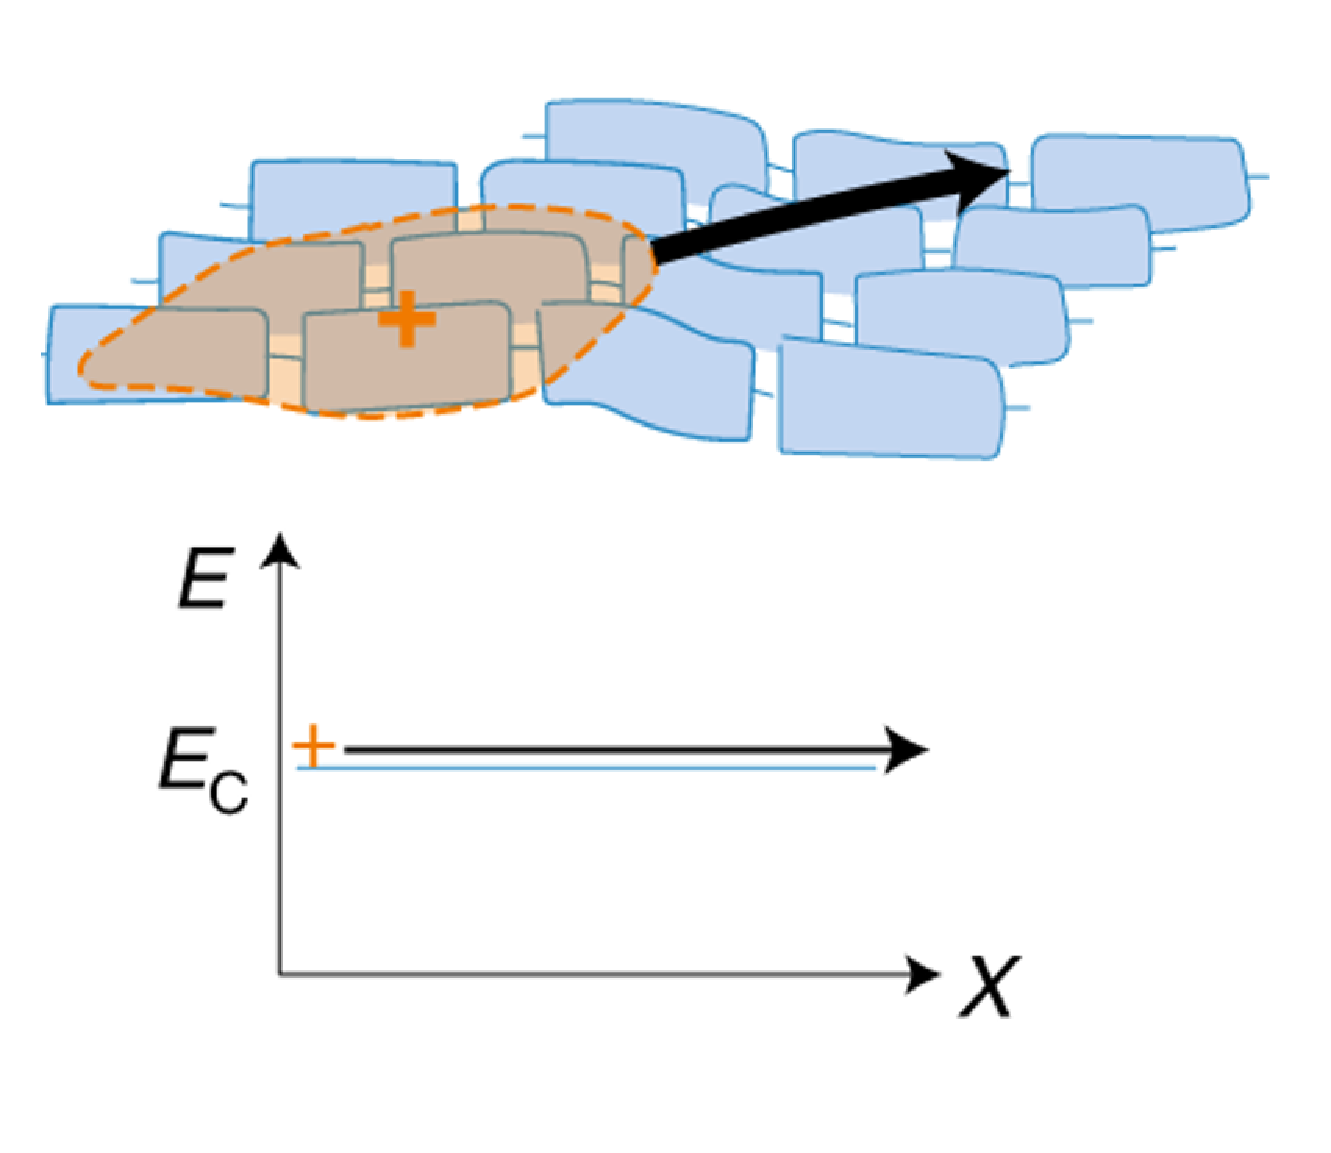
\includegraphics[width=5cm]{Images/pdf/OMIECetransport2.pdf} }}
	\caption[Electronic transport mechanisms in OMIECs]{Schematic representation of electronic charge transport mechanisms: a) Thermally-activated hopping transport %of a relatively localized electronic charge carrier" 
	and b) band-like transport, %of a relatively-delocalized electronic charge carrier"
	where the electronic charge carrier is relatively localized and delocalized, respectively. Extracted from reference \cite{paulsenOrganicMixedIonic2020}.} 
	\label{fig:etrans}
\end{figure}

Thermally-activated hopping, as its name implies, is driven by thermal energy and is limited by the degree of structural disorder. In this mechanism, weakly-bonded electrons in delocalized $\pi$-orbital move along adjacent $\pi$-orbitals within the length of the conjugated polymer, or even between molecules where there is sufficient $\pi$-$\pi$ overlapping. This mechanism predominates when there is a low electronic charge carrier density and a low density of accessible hopping states, resulting in low mobility and electrical conductivity \cite{paulsenOrganicMixedIonic2020}. 

In contrast, band-like transport, typically occurs in OMIECs with increasing doping levels. In this case, the activation energy of charge hopping decreases, and carrier mobility increases. This leads to diffuse band-like charge transport within the polymer-stacking \cite{wangHoppingTransportHall2012}.
%"at extreme doping levels, increased disorder drives carrier localization, which results in a plateau or even decrease in electronic charge carrier mobility"

%"Non-conjugated radical polymers also present a thermally activated mechanism of charge transfer between pendant radical sites, though with a significant dependence on the local self-diffusion of polymer chain to bring radical sites close enough for efficient charge transfer51. This manifests as a hopping transport of electronic carriers (Fig. 2a) that is assisted via segmental motion (described below; Fig. 2g). Also in this case disorder plays a role, producing local variations in the molecular orbital energy levels and spreading orbitals in a density of radical states52."


\subsubsection{Ionic transport}
While transport of anions and cations in OMIECs shares some similarities with the transport of electrons and holes, it is a more complex process, since ions can be \textit{``multi-valent, and form pairs and larger clusters; morever, they are sensitive to solvent and solvation''} \cite{paulsenOrganicMixedIonic2020}.

Ion transport in dry OMIECs of type I, III, and V is unipolar because these ions are fixed on a polyelectrolyte. In contrast, in type II, IV, and VI OMIECs, both anions and cations are mobile. When OMIECs come into contact with an electrolyte, they tend to swell, allowing the penetration of excess ions from the electrolyte. Therefore, both mobile anions and cations contribute to ion transport to ensure electroneutrality. 

\begin{figure}[!htb]
	\centering
	\subfloat[\textbf{Ion hopping} via segmental motion\\\hspace{1em} or ion clusters]{{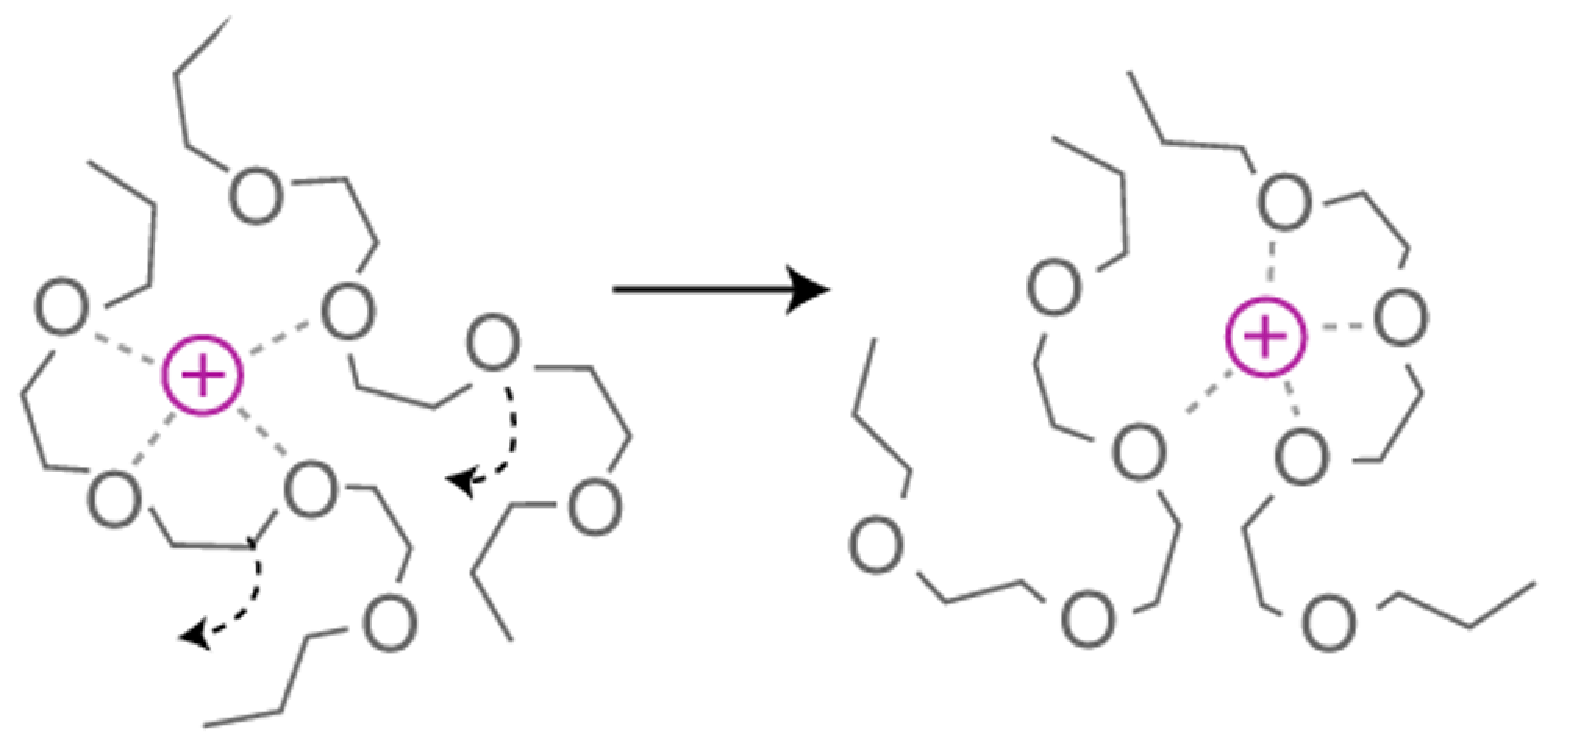
\includegraphics[width=7cm]{Images/pdf/OMIECitransport1.pdf} }}
	%\qquad
	\hspace{2em}
	\subfloat[\textbf{Solvated/vehicle mechanism}]{{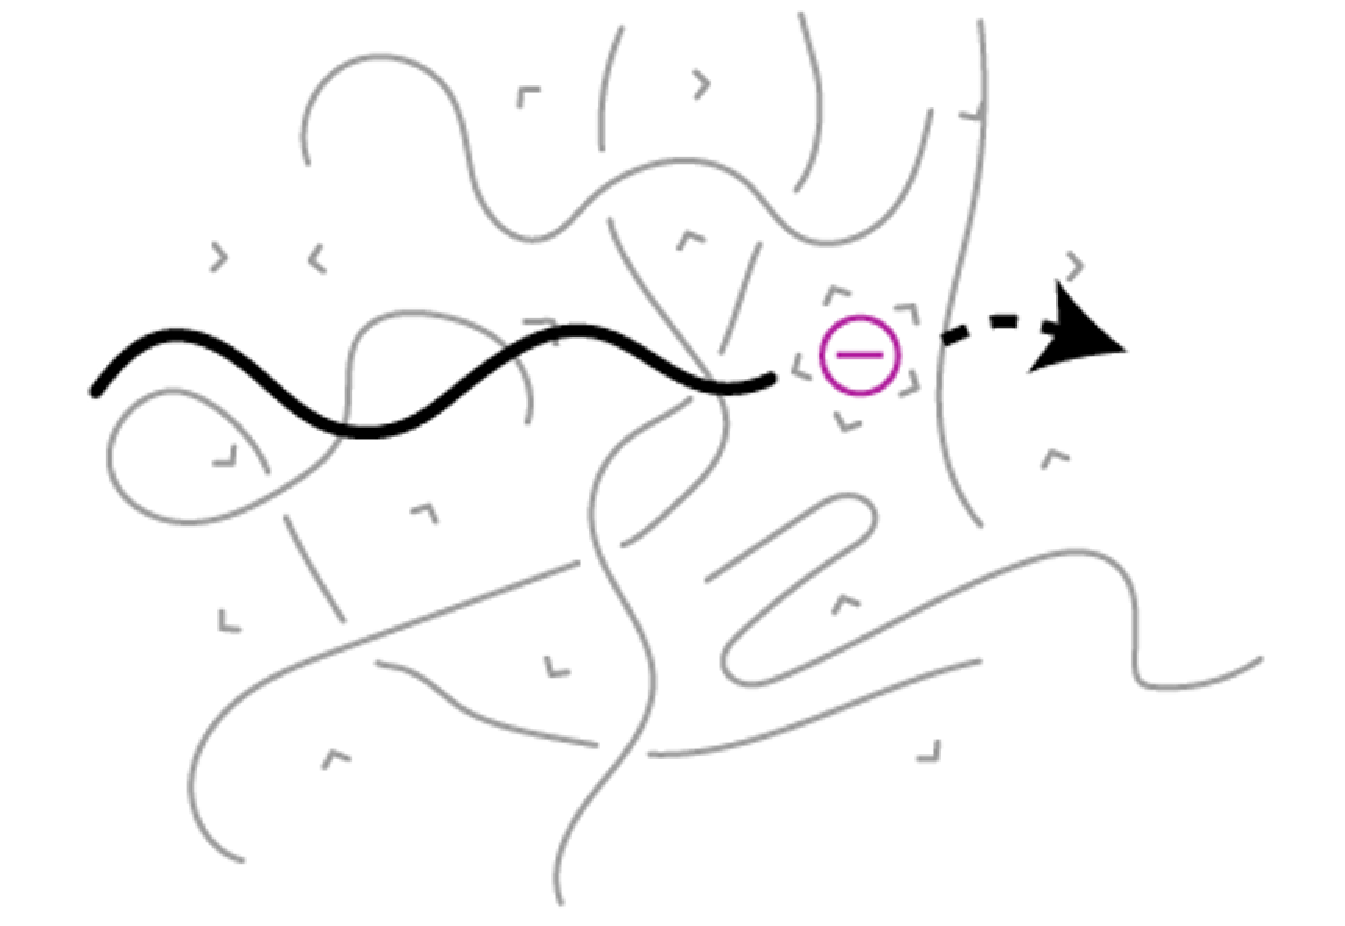
\includegraphics[width=5cm]{Images/pdf/OMIECitransport2.pdf} }}
	\caption[Ionic transport mechanisms in OMIECs]{Schematic representation of ionic charge transport mechanisms: a) Ion hopping via segmented motion and b) vehicular solvated-ion transport. Extracted from reference \cite{paulsenOrganicMixedIonic2020}.}
	\label{fig:itrans}
\end{figure}

There are two types of ionic charge transport in OMIECs: ion hopping and vehicular solvated-ion transport. In dry or minimally hydrated OMIECs, ion hopping assisted by segmental motion of the OMIEC side chains or backbone is the primary mechanism, as shown in Figure \ref{fig:itrans}A. However, when OMIECs are in contact with a solvent or liquid electrolyte, both mechanisms are present, with solvated ion vehicle transport being the predominant mode. For instance, in water-based electrolytes, proton diffusion occurs via the Grotthuss mechanism, where protons within water molecules diffuse through neighboring molecules. This involves a transfer of ionic effects through the hydrogen-bonded network, as shown in Figure \ref{fig:itrans}b.

Due to the existing ionic-electronic coupling, both ionic and electronic transport in OECTs and other OMIEC-electrolyte-based applications are not independent but are rather complex and must consider side effects such as hydration and electrolyte swelling \cite{paulsenOrganicMixedIonic2020}, as will be further discuss in Section \ref{sec:OECTs}.

%\subsection{Electrochemical Doping}

%As mentioned before, when OMIEC are coupled with an electrolyte and additionally, it is biased with an external gate, ionic-electronic interactions can be modulated. The OMIEC can oxidize or reduce depending on the mobile ions that penetrate the film, ions induced charges allowing its doping.

%Along the morphologic changes of the OMIEC, due to with the generation of permanent distortion in the lattice spacing and expansion in the lamellar direction and contraction in in the $\pi$-$\pi$ direction" \cite{cendraRoleAnionTransport2019}
 
%"The electrochemical charging of OMIECs can be described as a capacitive faradaic charging process,
% there is current caused by charge transfer, other physical phenomenas such as desorption or adsorption can also lead to the aparition of current that is non faradaic reaction
%meaning that the OMIEC" is p-doped (oxidized, in the language of chemists) "through an electron transfer with the contact (current collector), while ions from the electrolyte penetrate inside the channel material to compensate the charge carriers on the polymer backbone electrostatically with no change in the inserted ion's oxidation state" \cite{giovannittiEnergeticControlRedoxActive2020}

%"Electrochemical doping produces a permanent distortion in the lattice spacings, inducing an expansion in the lamellar direction and a contraction in the $\pi$-$\pi$ direction" \cite{cendraRoleAnionTransport2019}

\section{Organic Electrochemical Transistors} \label{sec:OECTs}

Organic Electrochemical Transistors are composed of metallic source, drain and gate electrodes, an organic conjugated polymer channel (specifically an OMIEC as described in previous sections), and an electrolyte that bridges the channel and the gate, as illustrated in Figure \ref{fig:bernard}a. OECTs are devices that have received increasing attention due to their mechanical compliance, biocompatibility, and sensitivity to biochemical signals \cite{tanMixedIonicElectronic2022}. 

%\begin{figure}[ht]
%	\centering
%	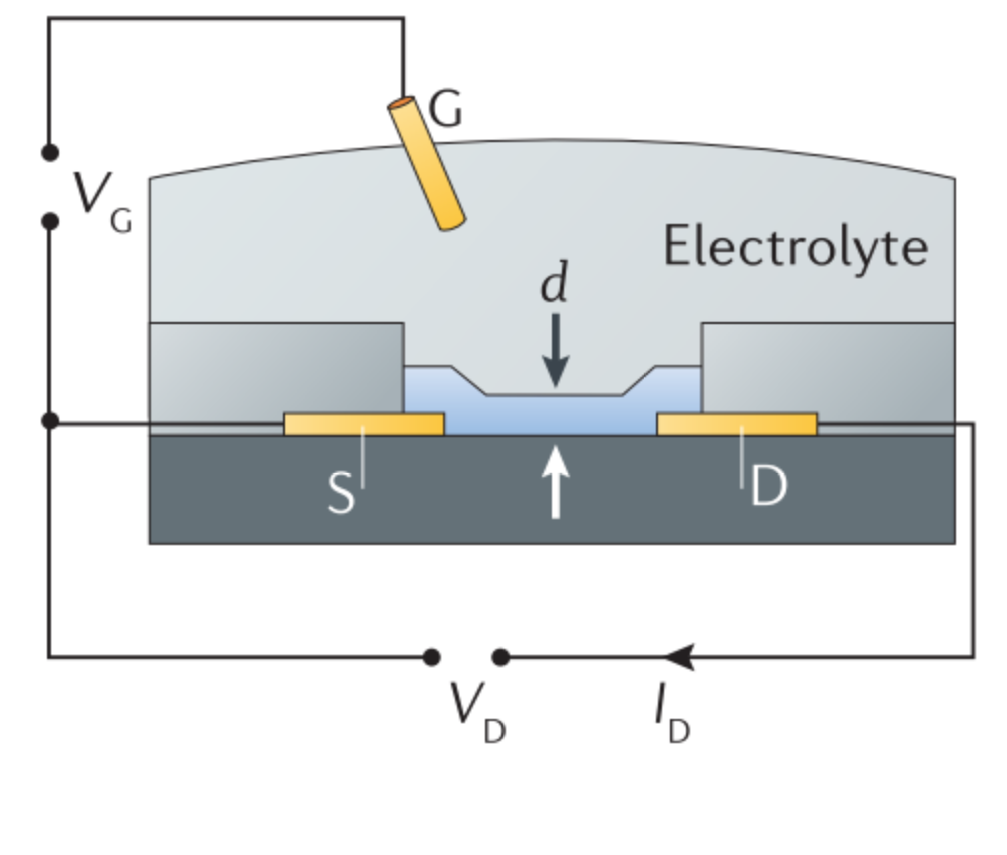
\includegraphics[height=4.5cm]{Images/structure.png}
%	\caption{Typical structure of an organic electrochemical transistor (OECT) \cite{rivnayOrganicElectrochemicalTransistors2018}.}
%	\label{fig:modes}
%\end{figure}


\subsection{Device Physics} \label{subsec:devphy}

Although the structural configuration of OECTs differs from conventional metal-oxide-semiconductor field-effect transistors (MOSFETs), understanding the operation of the latter can provide insight into how OECTs function. In contrast to MOSFETs, where an insulator is used, OECTs are coupled with an electrolyte, as shown in Figure \ref{fig:vsMOS}. When a gate voltage is applied, instead of polarizing the dipoles in the insulator and creating a field that causes accumulation of carriers at the interface of the semiconductor/insulator, as is the case with MOSFETs, in OECTs, the gate voltage drives ions to penetrate the bulk of the channel. Consequently, accumulation of carriers occurs throughout the whole volume of the OMIEC film. This mechanism explains the large gate-channel capacitance observed in these devices compared to MOSFETs and why the drain current takes into account a volumetric capacitance \cite{friedleinDevicePhysicsOrganic2018}.


\begin{figure}[ht]
  \centering
  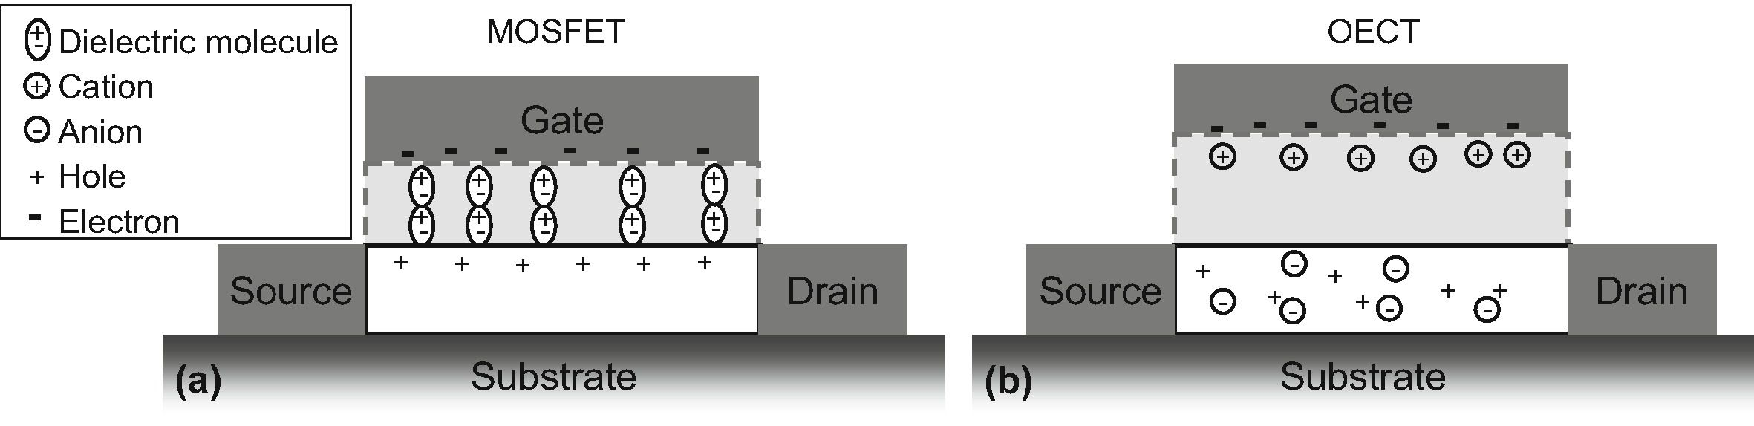
\includegraphics[width=\textwidth]{Images/pdf/MOSFETvsOECTs.pdf}
  \caption[Device physics of MOSFET vs OECT]{Comparison of p-type a) MOSFET and b) OECT, where the light-gray region represents an insulator and electrolyte, respectively. Extracted from reference  \cite{friedleinDevicePhysicsOrganic2018}}
  \label{fig:vsMOS}
\end{figure}

Bernards and Malliaras implemented a model based on a p-type depletion-mode OECT (based on PEDOT:PSS as it is widely studies and fabricated material, further discussion in the following section) \cite{bernardsSteadyStateTransientBehavior2007}. The model divides the behavior of the OECT into two circuits: an electronic circuit (comprising the source-channel-gate structure) and an ionic circuit (comprising the gate-electrolyte-channel structure).

The electronic circuit is treated as a \textit{variable} resistor and is thus modeled using Ohm's law. Its variability arises from the fact that when a positive gate voltage is applied, de-doping of the semiconductor occurs, which is analogous to the compensation doping observed in silicon. Cations from the electrolyte penetrate the polymer, compensating for an acceptor. 

Meanwhile, the ionic circuit consists of a resistor that represents the flow of ions in the electrolyte, connected in series with a capacitor representing the storage of ions in the channel, as shown in Figure \ref{fig:bernard}b  \cite{rivnayOrganicElectrochemicalTransistors2018}\cite{bernardsSteadyStateTransientBehavior2007}. 

\begin{figure}[ht]
	\centering
	\subfloat[Typical OECT structure]{{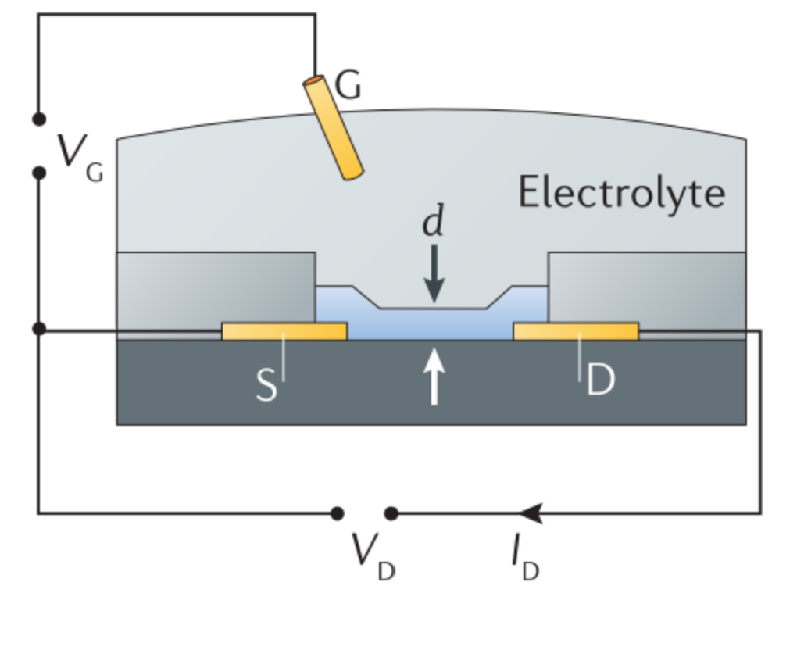
\includegraphics[width=4cm]{Images/pdf/structure.pdf} }}
	%\qquad
	%\subfloat[]{{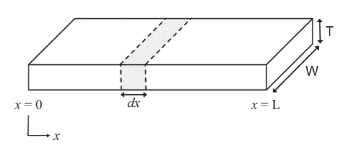
\includegraphics[height=1.5cm]{Images/film_model.png} }}
	%\subfloat[]{{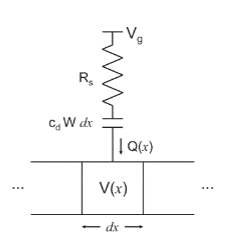
\includegraphics[height=4.5cm]{Images/circuit_model.png} }}
	\hspace{2em}
	\subfloat[Electronic and ionic circuits]{{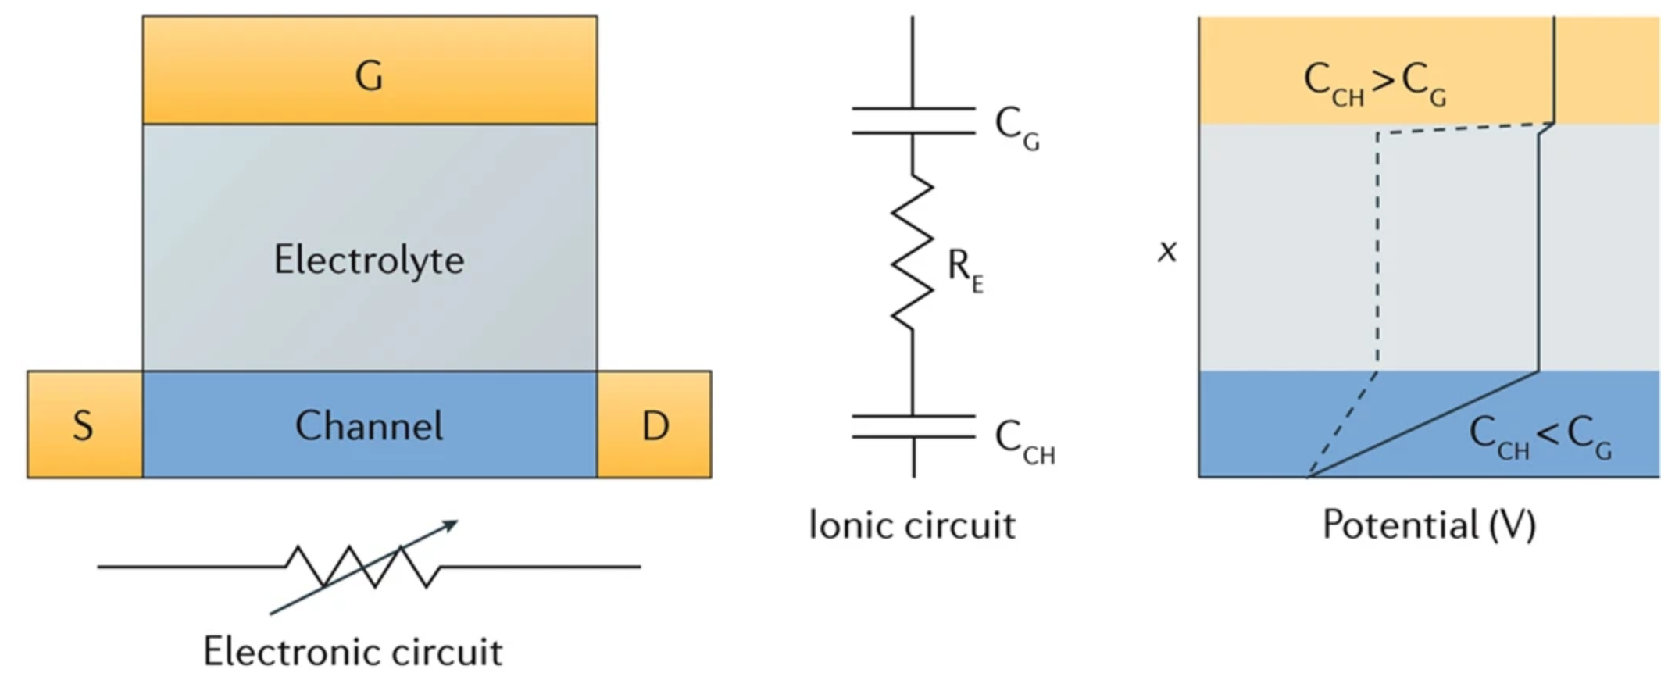
\includegraphics[width=8.5cm]{Images/pdf/circuits.pdf} }}
	\caption[Typical OECT structure and circuit model]{a) Typical structure of an organic electrochemical transistor. b) (Left) Electronic circuit modelled as a resistor with a varible resistance. (Right) Ionic circuit consisting of channel (C$_{CH}$) and gate (C$_{G}$) capacitors, coupled with a resistor corresponding to the electrolyte (R$_{E}$). Extracted from reference \cite{rivnayOrganicElectrochemicalTransistors2018}.}
	\label{fig:bernard}
\end{figure}

Finally, the drain current $I_{D}$ for the steady state behavior of the OECT can now be described using the following equation:

\begin{equation}\label{eq:id}
	I_{D} = \begin{dcases*}
    -\mu C^{*} [\frac{Wd}{L}\frac{V_{GS}-V_{Th}^{2}}{2V_{Th}}] & \text{$|V_{DS}| < |V_{GS}|-|V_{Th}|$} \\
    -\mu C^{*} \frac{Wd}{L} [1 - \frac{V_{GS}-1/2 V_{DS}}{V_{Th}}] V_{DS} & \text{$|V_{DS}| > |V_{GS}|-|V_{Th}|$}
    \end{dcases*}
\end{equation}

where $\mu$ is the charge mobility, C* is the volumetric capacitance and W, d and L are the width, thickness and length of the channel. $V_{GS}$, $V_{DS}$ and $V_{Th}$ correspond to the gate, drain and threshold voltage, respectively. Parameters will be further discuss in Section \ref{OECT:fom}.  

\subsection{Operation Modes}

Analogous to conventional MOSFETs, depending on whether the device requires a gate potential to be turned ON, OECTs exhibit two operation modes: depletion and enhancement (the latter often referred to as accumulation in the context of OECTs). The operation modes are closely linked to the nature of the channel material%if it is inherently conductive or semiconducting
.

\begin{figure}[ht]
	\centering
	\subfloat[Depletion-mode OECT]{{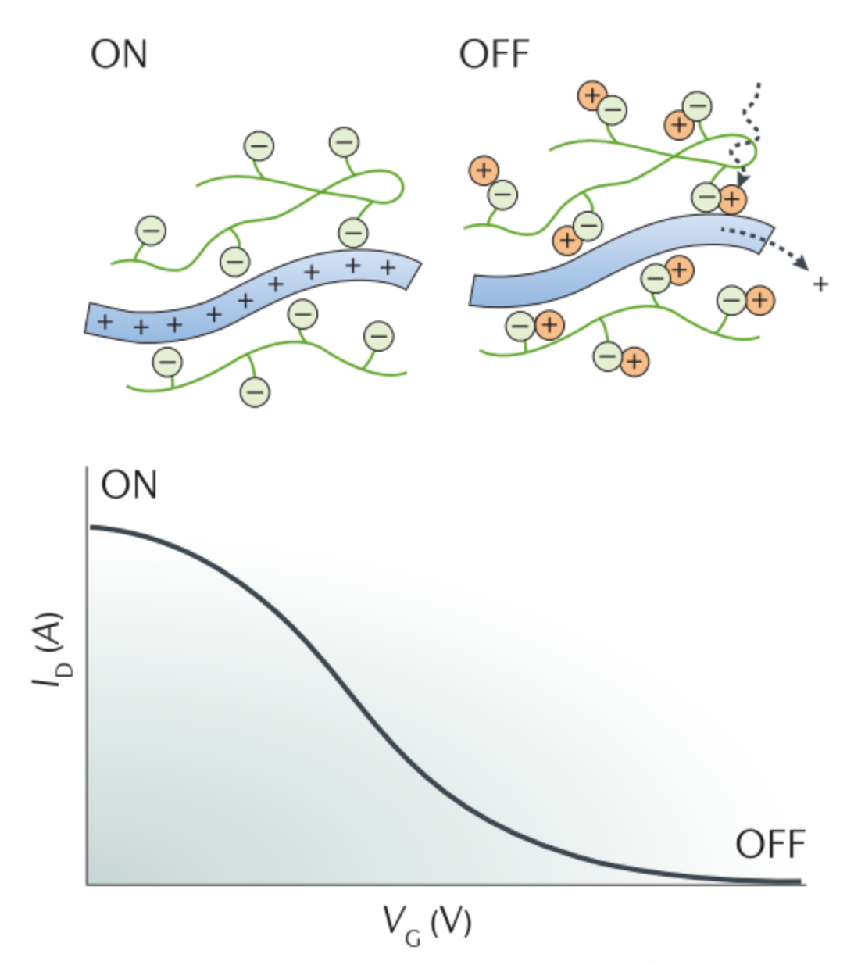
\includegraphics[height=7cm]{Images/pdf/depletion.pdf} }}
	\hspace{2em}
	\subfloat[Accumulation-mode OECT]{{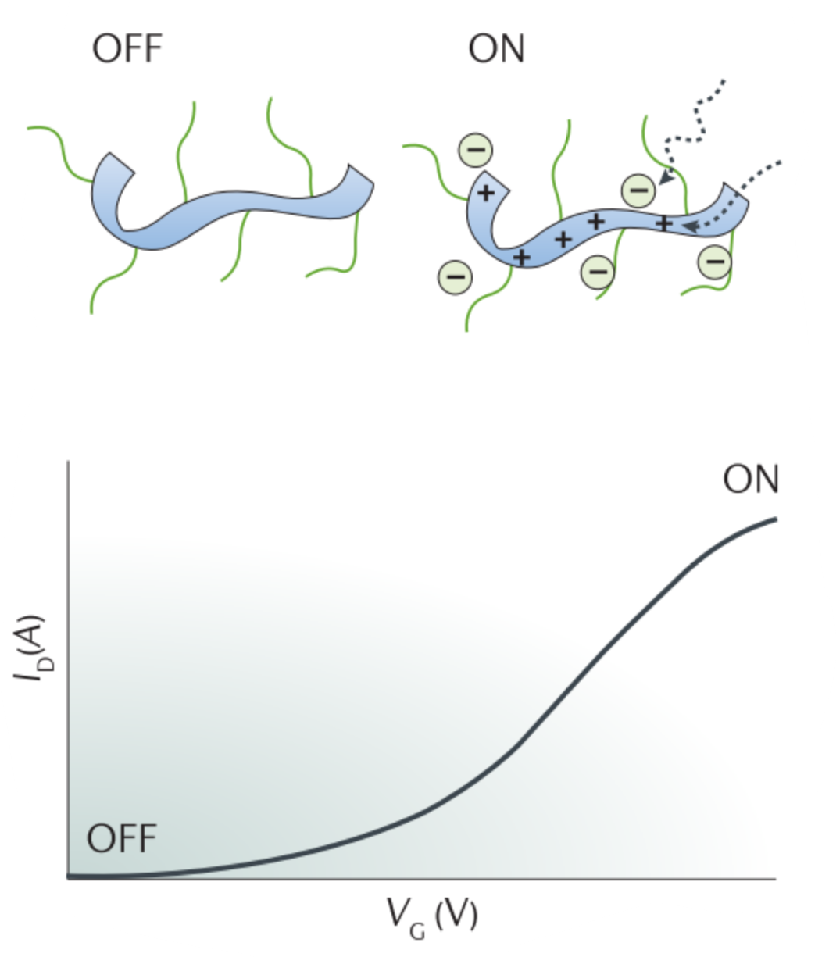
\includegraphics[height=7cm]{Images/pdf/accumulation.pdf} }}
	\caption[Depletion- and accumulation-mode OECTs]{a) Transfer curve showing depletion-mode operation of a p-type OECT with a conducting polymer channel. b) Transfer curve showing accumulation-mode operation of a p-type OECT with a insulating polymer channel. Images extracted from reference \cite{rivnayOrganicElectrochemicalTransistors2018}.}
	\label{fig:modes}
\end{figure}

As illustrated in Figure \ref{fig:modes}a and b, the polymer can be either intrinsically doped (conductive) or undoped (insulating). In the first scenario, the OMIEC already possesses anions that induce charges within its backbone. Consequently, to turn off the device, cations need to be injected to counteract this effect. Conversely, for an insulating polymer channel, a zero-gate biased OECT will have no charges induced in its backbone, resulting in the OFF state. To transition to the ON state, a gate voltage is required to drive anions into the polymer and induce charges.

\subsubsection{Standard material for depletion-mode OECTs}

Poly(3,4-ethylenedioxythiophene) poly(styrene-sulfonate) (PEDOT:PSS) is a \textit{``degenerately doped''} \cite{bernardsSteadyStateTransientBehavior2007} or conductive polymer that is widely used in various applications in organic electronics. Classified as type I OMIEC, as seen in Figure \ref{fig:omiectypes}, it is a blend between a conjugated polymer (PEDOT) and a polyelectrolyte (PSS), the latter possesses chemically linked ions and serves as a polymeric acid template to allow dispersable suspensions \cite{paulsenOrganicMixedIonic2020}.

Due to its commercial availability, operational stability, and relatively high performance, PEDOT:PSS became a standard material for p-type OECTs. However, its main drawback lays in its depletion-mode operation.

With the aim of minimizing power consumption, there is a strong interest in fabricating high-performance accumulation-mode devices \cite{nielsenMolecularDesignSemiconducting2016}\cite{tanOrganicMixedIonic2022}\cite{inalBenchmarkingOrganicMixed2017}\cite{keeneEnhancementModePEDOTPSS2020}. These devices offer the advantage of dissipating less static power when the device is not in operation, due to low OFF current %, which must be minimized as much as possible
\cite{giovannittiEnergeticControlRedoxActive2020}.

\subsubsection{Prospective materials for accumulation-mode OECTs}
% As a widely studied material, 
PEDOT:PSS has not been ruled out as a possible accumulation-mode OECT, Keene et al. employed a series of amines to de-dope PEDOT:PSS and achieve OECTs with negative turn-on voltages \cite{keeneEnhancementModePEDOTPSS2020}. However, synthetically modifying PEDOT:PSS in a controlled manner remains a challenge. 

In parallel to these efforts, researchers are also working on the design of new conjugated polymers with the aim of not only having accumulation-mode OECTs but enhancing their performance. Nielsen et al. reported a series of semiconducting polymers with triethylene glycol (TEG) side chains, some of which demonstrated good performance. Among the five thiophene- and benzodithiophene-based polymers, they found out that the one with a %TEGylated 
backbone consisting of 2,2'-bithiophene (blue) polymerized with other thiophene molecule (green), named as \textbf{g2T-T}, as seen in Figure \ref{fig:g2TT}, exhibited the highest performance %, even higher transconductance over PEDOT:PSS
\cite{nielsenMolecularDesignSemiconducting2016}.

\begin{figure}[ht]
	\centering
	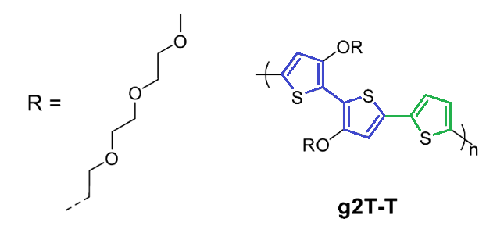
\includegraphics[width=7cm]{Images/pdf/g2T-T.pdf}
	\caption[Chemical structure of polymer g2T-T]{Chemical structure of polymer with backbone g2T-T, R representing the side chain. Extracted from reference \cite{nielsenMolecularDesignSemiconducting2016}.}
	\label{fig:g2TT}
\end{figure}

Moser et al. conducted a study using the same backbone (g2T-T) to investigate the impact of the length of the ethylene glycol (EG) side chain on the performance of OECTs 
\cite{moserEthyleneGlycolBasedSide2020}. They found that reducing the side chain length maximized both the capacitance and mobility of the OECTs. However, a shorter side chain is less favorable for ion-polymer interaction. 

Their research suggested an optimum-side-chain length of 3 monomers, compared to 2, 4 and 6 monomer. OECTs based on 3-(2-(2-(2-methoxyethoxy)ethoxy)ethoxy) thiophene (p(g3T2-T)) exhibited a turn-on voltage close to zero and superior performance compared to other thiophene-based species (as seen in Figure \ref{fig:pg3t} and Table \ref{tab:perf}), even surpassing PEDOT:PSS-based OECTs \cite{inalBenchmarkingOrganicMixed2017}. %. This advantage does not remain the only one, since p(g3T2-T)  would not require extensive pre- and postprocessing to optimize stability and electrochemical performance in aqueous media as PEDOT:PSS
%% actually the last part came from references 14-16 of that papers..

\begin{figure}[ht]
	\centering
	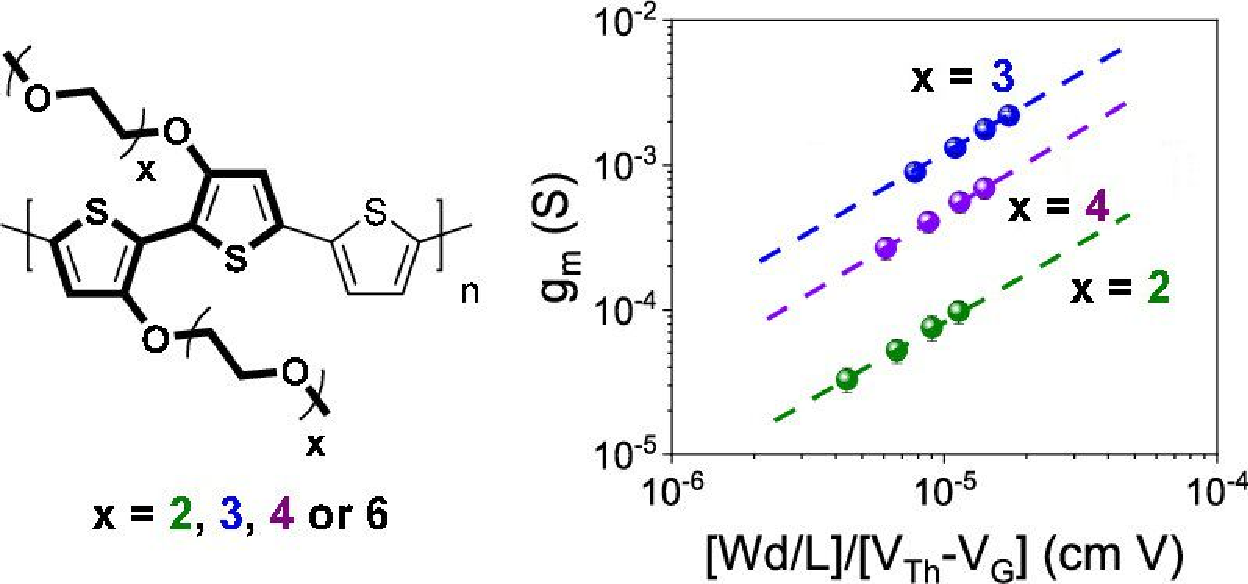
\includegraphics[width=10cm]{Images/pdf/pg3t+perf.pdf}
	\caption[Chemical structure and transconductance of g2T-T with side-chain engineering]{(Left) Chemical structure of the repeat units for p(gxT2-T). (Right) Transconductance vs channel geometry and operating parameters of p(gxT2-T) for x = 2, 3 and 4. Extracted from reference \cite{moserEthyleneGlycolBasedSide2020}.}
	\label{fig:pg3t}
\end{figure}

The structure of the polymer was designed to have a backbone that warrants reversibility during electrochemical redox reactions and good electronic transport, while the side chains enhance its stability in aqueous electrolytes and facilitate efficient transport of both ionic and electronic charge carrier \cite{moiaDesignEvaluationConjugated2019}. 
%% moia es el unico que tiene un dibujo distinto de pg3t
%Additionally, , and the absence of extensive pre- and postprocessing to optimize polymer stability and electrochemical performance in aqueous media %and the possibility of an accumulation-mode OECT with low operation voltages put it on top of compared to PEDOT:PSS \cite{moserEthyleneGlycolBasedSide2020}.

%Seria chevere tener un grafico de como thiophene publications empezaron a crecer.
%Thiophene is a planar conjugated ring structure consists of six delocalized pi-electrons. The aromatic nature arises from the four $\pi$-electrons and one unshared lone pair of electrons of the oxygen as six delocalized $\pi$-electrons. It folow Hucke´s rule. Hence it is aromatic compound.

%Homogeneous single phase OMIECs (types V and VI) display larger magnitudes of ionic–electronic coupling and larger values of volumetric capacitance than biphasic OMIECs (types I–IV) \cite{paulsenOrganicMixedIonic2020}. 

Under the classification presented in Figure \ref{fig:omiectypes}, p(g3T2-T) can be categorized as a type VI OMIEC that consists of a conjugated polymer with ions introduced as free species. Wheareas, PEDOT:PSS contains ions that are chemically linked to the polyelectrolyte (PSS). This structural distinction results in p(g3T2-T) displaying larger magnitudes of ionic-electronic coupling and volumetric capacitance compared to biphasic OMIECs like PEDOT:PSS \cite{paulsenOrganicMixedIonic2020}. Understanding these structural characteristics is crucial for addressing the challenges associated with achieving stable OECTs, as it will be further addressed in this thesis.%, further discussion in Section \ref{subsec:sidereac}.
%% Replace further discussion for a table with numbers of the two polymers

\begin{table}[ht]
	\centering
	\caption[Volumetric capacitance (C*) of various OECTs channel materials]{Volumetric capacitance (C*) of OECTs channel materials including p(g2T2-T), p(g3T2-T), p(g4T2-T) and PEDOT:PSS using a 0.1 NaCl electrolyte and Ag/AgCl pellet electrode.}
	\begin{tabular}{l c c} \hline
		Polymer	&  C* (Fcm$^{-3}$) & Reference \\ \hline
		p(g2T2-T) & 8$\pm$2 & \cite{moserEthyleneGlycolBasedSide2020}\\
		p(g3T2-T) & 211$\pm$18 & \cite{moserEthyleneGlycolBasedSide2020}\\
		p(g4T2-T) & 192$\pm$10 & \cite{moserEthyleneGlycolBasedSide2020}\\  
		PEDOT:PSS & 39 & \cite{inalBenchmarkingOrganicMixed2017}\\\hline
	\end{tabular}
	\label{tab:perf}
\end{table}


\subsection{Important Figures of Merit} \label{OECT:fom}

\subsubsection{Transconductance}
Transconductance is considered as the most important parameter for measuring the amplification capability of any transistor. It is calculated as the first-order derivative of the output current (drain current) with respect to the input voltage (gate-source voltage), expressed as $g_{m} = \sfrac{\partial I_{D}}{\partial V_{GS}}$. Bernards and Malliaras derived this parameter in their mathematical model for depletion-mode p-type OECTs \cite{bernardsSteadyStateTransientBehavior2007}, as discussed in Section \ref{subsec:devphy}. When considering both n-type and p-type OECTs, the transconductance can be expressed as follows: %\ref{eq:gm}:

\begin{equation}\label{eq:gm}
	g_{m} = \frac{Wd}{L} \mu C^{*} |(V_{th} - V_{G})|,
\end{equation}

where $W$, $L$ and $d$ are the channel width, length, and thickness, respectively, $\mu$C* denotes the product of mobility and volumetric capacitance, while $V_{G}$ and $V_{th}$ stand for the gate voltage and threshold voltage, which will be further discussed in the following subsections.

Typically, the maximum transconductance ($g_{m,max}$) is reported, which falls into the saturation regime. Inal et al. reported the maximum transconductance for various channel materials with different device geometry parameters. They used an Ag/AgCl pellet as reference/gate electrode and 0.1M NaCl as electrolyte. Their results showed that OECTs with polymerized g2T backbones exhibited the best performance, achieving transconductance values ranging from 1 to 30 mS, depending on the geometry (Figure \ref{fig:gmuc}a) \cite{inalBenchmarkingOrganicMixed2017}.

\subsubsection{$\mu$C* product}

The parameter $\mu$C* is considered the most important for benchmarking OECT channel materials because it represents both the ionic and electronic transport properties %storage ability
\cite{inalBenchmarkingOrganicMixed2017}. %\cite{inalHighTransconductanceAccumulation2014}. %% Other accumulation mode OECT with PTHS
It is the product of two important parameters, $\mu$, the electronic mobility, and C*, the volumetric capacitance, the latter encloses the ion penetration, transport, and storage ability of the OMIEC film.

Along with the transconductance, Inal et al. determined the values of $\mu$C* by calculating the linear slope of the maximum transconductance and channel geometry (Figure \ref{fig:gmuc}a), using Equation \ref{eq:gm}. They correlated their results with independent calculations of both parameters and found that polymerized g2T backbones exhibited the highest $\mu$C* value of 261 $\pm$ 29 $Fcm^{-1}V^{-1}s^{-1}$. Among the materials that showed a close 1:1 relationship for both methods of calculation of the $\mu$C* product, polymerized g2T backbones stood out (Figure \ref{fig:gmuc}b) \cite{inalBenchmarkingOrganicMixed2017}.
 
 \begin{figure}[ht]
 	\centering
 	\subfloat[]{{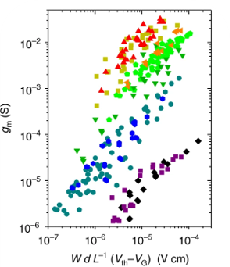
\includegraphics[width=4.5cm]{Images/pdf/gm_sizes.pdf} }}
 	\hspace{2em}
 	\subfloat[]{{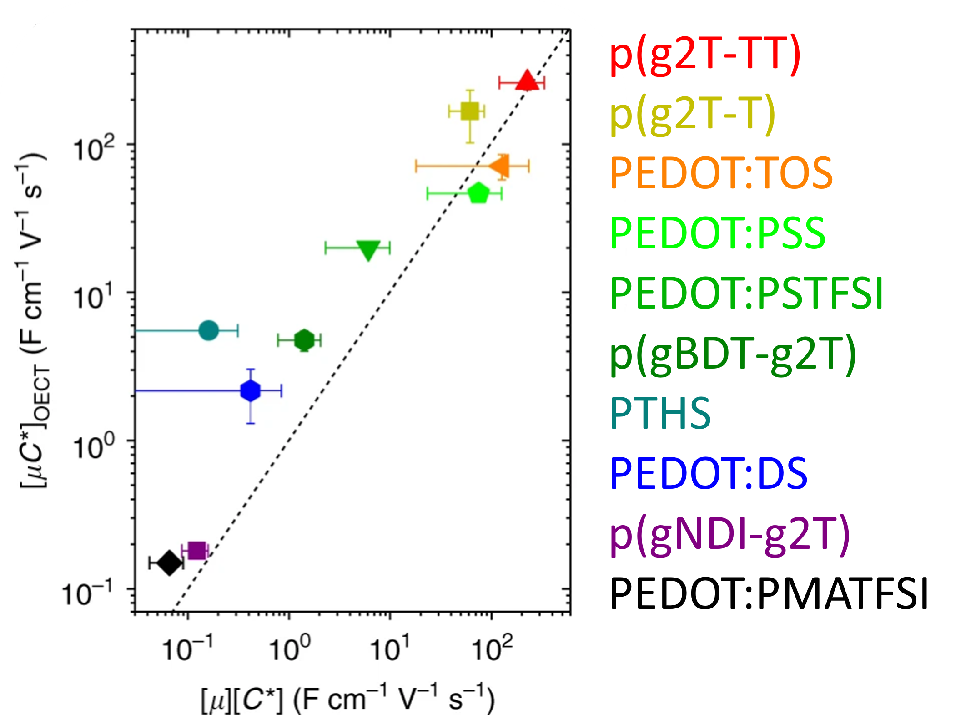
\includegraphics[width=7cm]{Images/pdf/uc_omiecs.pdf} }}
 	\caption[OECTs benchmark with different OMIECs]{a) Plot of $\mu$C* product calculated by the linear slope between transconductance and channel geometry. b) Calculated slope from a) in function of the product of independent determination of $\mu$ and C*, dotted line represents the 1:1 relation between both methods of calculation. Extracted from reference %\cite{ohayonSaltsAdditivesRoute2023} 
 		\cite{inalBenchmarkingOrganicMixed2017}.}
 	\label{fig:gmuc}
 \end{figure}

Calculating the electronic mobility ($\mu$) independently is challenging due to the presence of ionic species. This calculation is normally performed in transient regimes, taking advantage of ions' lower mobility, but it is outside the scope of this work. 

One method to calculate the volumetric capacitance (C*) is by performing Electrochemical Impedance Spectroscopy (EIS). Equation \ref{eq:C} is used to calculate the capacitance (C) based on the imaginary part of impedance ($Z^{img}$) at low frequency ranges where the capacitance should describe a plateau. %,since the modulation of AC is slow enough to fully populate the OMIEC with ions.
The calculated capacitance is then divided by the film volume to obtain C* %. Another approach is to use cyclic voltammetry (CV)
 \cite{ohayonGuideCharacterizationOrganic2023}.

\begin{equation} \label{eq:C}
	C = \frac{1}{2\pi \cdot f \cdot |Z^{img}|},
\end{equation}

%The calculation of this capacitance is under a fixed-gate biased condition, 
It is important to note that the capacitance (C) can be potential-dependent when electrochemical doping is modulated in OECTs with an applied bias %. Homogeneous single phase OMIECs (type V and VI) display larger magnitudes of ionic-electronic coupling and larger values of volumetric capacitance than biphasic OMIECs such as PEDOT:PSS 
\cite{inalBenchmarkingOrganicMixed2017}.
% found in Paulsen \cite{paulsenOrganicMixedIonic2020}
%actually from reference 44, benchmarking omiecs for transistors

\subsubsection{Threshold voltage}

The threshold voltage ($V_{th}$) in an OECT can be determined from the steady-state transfer characteristics ($I_{D}$ vs $V_{GS}$). To calculate $V_{th}$, you can plot the square root of $I_{D}$ as a function of $V_{GS}$ and extrapolate the linear portion of the slope, where it intersects the x-axis. This value of $V_{th}$ represents the \textit{``film's readiness for ion penetration''} in OECTs \cite{ohayonGuideCharacterizationOrganic2023}.

Controlling or shifting the threshold voltage is desirable, specially for integrating transistors into circuits to meet specific requirements for operation, noise margins, and power consumption. There are different approaches to achieve this. One approach is the chemical de-doping of PEDOT:PSS, as discussed in previous sections, which can shift the threshold voltage to negative values characteristic of accumulation-mode OECTs \cite{keeneEnhancementModePEDOTPSS2020}. 

 \begin{figure}[ht]
	\centering
	\subfloat[]{{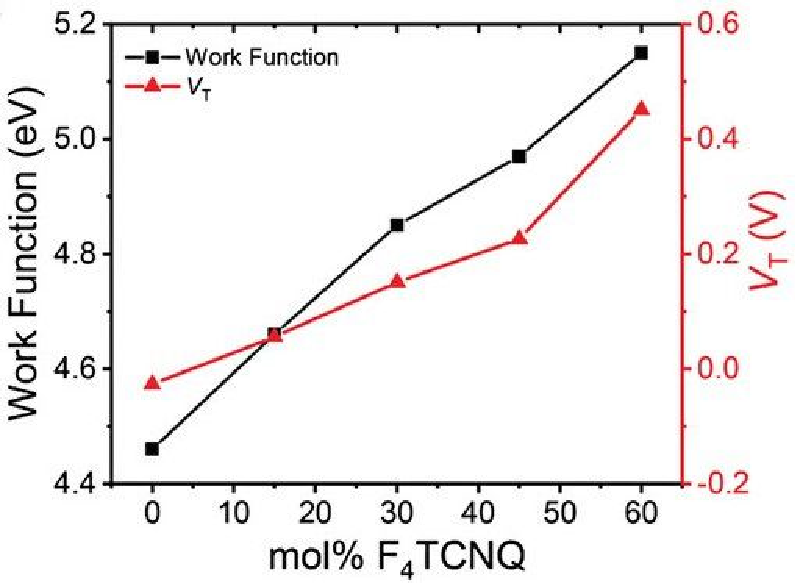
\includegraphics[width=5.8cm]{Images/pdf/wf_shift.pdf} }}
	\hspace{2em}
	\subfloat[]{{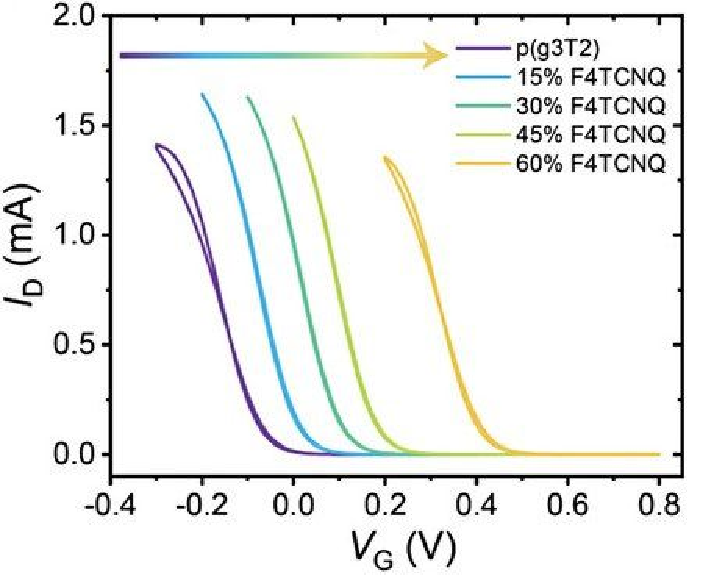
\includegraphics[width=5cm]{Images/pdf/vth_shift.pdf} }}
	\caption[Tuning of threshold voltage with different levels of doping p(g3T2-T)]{Controlling OECT threshold voltage by chemical doping of p(g3T2-T) gate electrode with F$_{4}$TCNQ. a) Plot of threshold voltage and gate work function for doped gates of different dopant concentrations. b) Transfer curves of p(g3T2-T) channel OECT %(L = 10 µm; W = 2000 µm; VD = −0.1 V, VG scan rate of 20 mV s−1) 
	with p(g3T2-T) gates of various F$_{4}$TCNQ dopant concentrations. Extracted from reference \cite{tanTuningOrganicElectrochemical2022}.}
	\label{fig:tune}
\end{figure}

Another approach, explored by Tan et al., involves tuning the doping level of the gate to shift the threshold voltage. They used p(g3T2-T) and achieved a 400 mV change in threshold voltage with a 60\% molar ratio of %2,3,5,6-Tetrafluoro-7,7,8,8-tetracyanoquinodimethane (
F$_{4}$TCNQ dopant, as shown in Figure \ref{fig:tune}. This approach offers advantages such as i) protecting the material from oxidation by bringing the Fermi level towards the highest occupied molecular orbital, and ii) avoiding interference with the channel which helps to maintain the transconductance unaffected \cite{tanTuningOrganicElectrochemical2022}.


\subsection{Side Reactions} \label{subsec:sidereac}

%Achieving effective charge transfer between the analyte and OMIEC requires appropriate alignment of the electrochemical potential of electrons on the OMIEC electrode and the redox specie. Failure to do so may result in the subsequent transfer of charges to other redox-active sinks in the environment, leading to undesirable side reactions and products that may interfere with the OMIEC’s operation. Electrons flow from a region of higher to lower electrochemical potential. Hence, achieving electron transfer from redox-active species to the OMIEC requires the latter to have a deep LUMO (high electron affinity) \cite{tanMixedIonicElectronic2022} %paper

%Capacitive fading upon cycling

\subsubsection{Water uptake and swelling}

%Although there are some studies in non-water-based electrolytes, such as ionic liquids. 
Water uptake and swelling are important side reactions that occur when OMIECs come into contact with water-based electrolytes. Even in the pursuit of solid-state OECTs, precursors may contain a certain degree of water content  \cite{weissbachPhotopatternableSolidElectrolyte2022}\cite{nguyen-dangBiomaterialBasedSolidElectrolyteOrganic2021}, making it necessary to understand the impact of water-related side reactions. %and some bioelectronics applications will inevitable operate under water environment, 

Water uptake in OMIECs causes their increase of mass (swelling) and changes in morphology. This water uptake occurs because OMIECs need to compensate for their intrinsic doping, and as a result, \textit{``the effect of doping-induced hydration on the OMIEC morphology must be taken into account when designing OECTs''} \cite{savvaBalancingIonicElectronic2020}.

Savva et al. conducted an study to investigate the influence of water on the performance of PEDOT:PSS OECTs. They found that water uptake %of conjugated polymer films 
led to a 10-13\% increase in mass under non-biased conditions. Interestingly, the concentration of water played a role in the ionic charging rate. While lower concentrations of water (NaCl$_{aq}$ 10 mM, 100mM, 1M, and 6M) led to faster ionic charging, %regardless of the doping pulse, 
the fastest %ionic charging 
response time was achieved with NaCl$_{aq}$ 1 M. This was attributed to attractive forces between counter ions, which % the injection/drift of ions is also affected by the ion-counterion, attractive forces in NaCl$_{aq}$ 6 M 
hindered the drift of anions and delayed the injection of ions from the electrolyte %, opposing their drift into the polymer affecting the response time. %Water irreversibly changes the film morphology, In general, while ion transport is enhanced, electronic charge transport is negatively impacted 
\cite{savvaInfluenceWaterPerformance2019}.

%Swelling is produced due to the compensation doping in the film, the ratio of swelling is normally reported and calculating by measuring the length of  by estimating "the number of electrolyte ions compensating for the electronic charge carriers" in the OMIEC. \cite{ohayonGuideCharacterizationOrganic2023}. %Savva et al. demonstrated that polymers in contact with water and are used for enhancement mode OECTs detriment its electronic charge transport, since water irreversibly changes the film morphology, but at the same time enhances ion transport \cite{savvaInfluenceWaterPerformance2019}

%\subsubsection{Water uptake}
Another study by Savva et al. showed that a certain level of hydration is necessary for facile ionic transport, but can have a negative impact on electronic charge transport, particularly in glycol-based side chains \cite{savvaBalancingIonicElectronic2020}. These side chains are commonly used in accumulation-mode OECTs, where ionic transport is already enhanced through side-chain engineering \cite{moiaDesignEvaluationConjugated2019}. %increased its transconductance by five orders of magnitude, due to an increase in C* and charge carrier mobility. %\cite{siemons}


\subsubsection{Oxygen Reduction Reaction (ORR)}

The Oxygen Reduction Reaction (ORR) is a common undesirable side reaction that occurs under environmental conditions, especially in devices fabricated with polymers having low ionization potential (IPs). The use of OMIECs with low IPs is frequent in accumulation-mode OECTs. 


%With the aim of developing accumulation-mode OECTs, the engineering of new OMIECs were introduced as commented in previous sections. Normally, this polymer backbones have low ionization potential (IPs) which lead to another side effect issue that little attention has been paid: non capacitive faradaic rections in ambient: electron-transfer reaction from the OMIEC to molecular oxygen described as oxygen reduction reaction (ORR)

% Remember 
% Thermodynamically favored processes or reactions are those that involve both a decrease in the internal energy of the components (ΔH° < 0) and an increase in entropy of the components (ΔS° > 0). These processes are necessarily “thermodynamically favored” (ΔG° < 0) or negative. ΔG° = ΔH°-TΔS°
% Catalyst help to reduce the activation energy required for a reaction
The ORR is a non-capacitive faradaic reaction that takes place between the OMIEC and molecular oxygen, involving electron-transfer. This reaction can yield either hydrogen peroxide (H$_{2}$O$_{2}$) or water (H$_{2}$O), as described in \ref{eq:h2o2} and \ref{eq:h2o}, or it can result in the oxidation (p-doping) of the OMIEC which acts as the catalyst \cite{giovannittiEnergeticControlRedoxActive2020}. 

%The first shows a free energy difference that is endergonic for OMIECs with IPs > 4.9eV and hence prevent the OMIEC from undergoing ORR that form H$_{2}$O$_{2}$. To prevent the ORR in ambient conditions, OMIECs based on donor-acceptor copolymer (Type III or IV) that have large IPs to shift

% Actually this material does not avoid this, we need to take into account this interaction.


\begin{equation}\label{eq:h2o2}
	{E^{0}}_{O_{2}/H_{2}O_{2}} : O_{2} + 2H^{+} + 2e^{-} \rightarrow H_{2}O_{2}
\end{equation}

\begin{equation}\label{eq:h2o}
	{E^{0}}_{O_{2}/H_{2}O} : O_{2} + 4H^{+} + 4e^{-} \rightarrow 2H_{2}O
\end{equation}

As represented in Figure \ref{fig:orr}, $\eta_{1}$ and $\eta_{2}$ represent the free energy difference between reactants and the reaction products H$_{2}$O$_{2}$ and H$_{2}$O, respectively. If this free energy difference is negative, indicating that the reaction requires an energy input, the ORR is endergonic, while a positive free energy difference makes it exergonic (spontaneous). For instance, to prevent the formation of oxygen peroxide, a polymer with higher IP (> 4.9eV) would be required. 

In the context of OECTs, where polymers like PEDOT:PSS and p(g3T2-T) are used, it is important to recognize that these materials exhibit exergonic reactions under environmental conditions. Therefore, it is crucial to consider the impact of the ORR on device stability and performance, particularly in applications where long-term reliability is essential.

%\newpage
\begin{figure}[!ht]
	\centering
	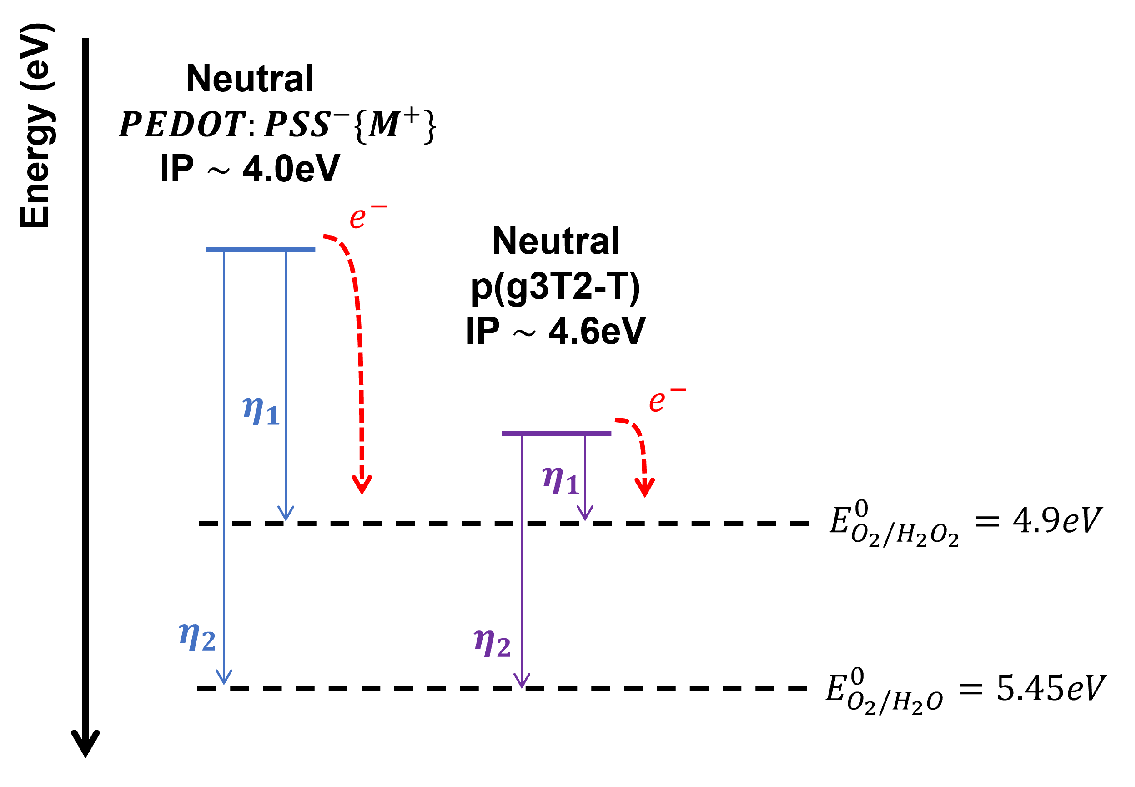
\includegraphics[width=10cm]{Images/pdf/ORR.pdf}
	\caption[Energy levels of neutral state of OMIECs related to oxygen reduction reactions potentials]{Simplified mechanism of two- and four-electron Oxygen Reduction Reactions with neutral states of OMIECs: p(g3T2-T) and PEDOT:PSS. The free energy difference between reactant and the reaction products is represented by $\eta$. Image adapted from reference \cite{giovannittiEnergeticControlRedoxActive2020}, where values are defined from cyclic voltammetry measurements using Ag/AgCl as reference electrode and NaCl as electrolyte.}
	\label{fig:orr}
\end{figure}

%\subsection{Photo-patternable Solid-State OECTs}

%\subsection{Building Block for neuromorphic and bioelectronic applications}


%%% Local Variables: 
%%% mode: latex
%%% TeX-master: "thesis"
%%% End: 

\chapter{Experimental Methods} \label{cha:2}
%\lipsum[77]

\section{Materials}
%\lipsum[78]
All reactives were purchased from commercial suppliers. %and non further chemical modification or purification was done unless stated before.

\begin{itemize}
\item Chromium etchant: High purity ceric ammonium nitrate, Standard, Sigma Aldrich
\item Gold etchant:  HHPAA (2-Hydroxy-4’-(2-hydroxyethoxy)-2-methylpropiophenone), 98$\%$, Standard, Sigma Aldrich
\item Developer: AZ 726 MIF Developer, Merck performance Materials GmbH
\item EG: Ethylene glycol, $\geq$ 95$\%$, Sigma Aldrich
\item $[$EMIM$][$EtSO$_{4}]$: (1-Ethyl-3-methylimidazolium ethyl sulfate), $\geq$95$\%$, Sigma Aldrich 
\item MBBAm: (N,N’-Methylenebisacrylamide), 99$\%$, Sigma Aldrich 
\item NIPAm: (N-Isopropylacrylamide), 97$\%$, Alfa Aesar 
\item Sacrificial Layer 1: Sacrifical Layer 1 (SL1), Orthogonal Inc
\item Photoresist: AZ 1518 Photoresist, Merck Performance Materials GmbH \& Microchemical GmbH
\item Photoresist for undoped species: NLOF 2020, commercial negative-tone photoresist, Microchemical
\item Orthogonal Photoresist for doped species: OSCoR 4020 Photoresist, Orthogonal Inc.
\item Developer for SL1: Developer HF 7300, Orthogonal Inc.
\item Orthogonal Developer for OSCor 4020: Orthogonal Developer 103a, Orthogonal Inc.
\item Orthogonal Stripper: Orthogonal Stripper 900, Orthogonal Inc. 
\item p(g3T2-T): 3-(2-(2-(2-methoxyethoxy)ethoxy)ethoxy)thiophene from Professor Iain McCulloch, Chemistry Research Laboratory, University of Oxford. 
\item Dopants: 1,3,4,5,7,8-hexafluorotetracyanonaphthoquinodimethane (F$_{6}$TCNNQ) and 1,3,4,5-tetrafluorotetracyanonaphthoquinodimethane (F$_{4}$TCNQ), 97$\%$, Sigma Aldrich.
\item Adhesion promoter: Silane A174 (3-(Trimethoxysilyl)propyl methacrylate), TCI.

\end{itemize}

\section{Equipment}
\begin{itemize}
\item Baking: All baking steps were carried out on a Stuart SD160 digital hotplate (Stuart Equipment, UK). 
\item Electrical characterization (ambient): Device characterization under ambient conditions was performed on a Everbeing C-6 Probe Station (Everbeing Int’l Corp., Taiwan), connected to a Keithley 4200-SCS Semiconductor Characterisation System (Keithley Instruments, USA). 
\item Electrical characterization (glovebox): Device characterization was performed in a nitrogen-filled glovebox. Probing needles were connected to two Keithley 236 Source Measure Units (Keithley Instruments, USA). 
\item Cyclic voltammetry and Impedance measurements: Measurements were carried out by using a Metrohm Autolab PGSTAT302N potentiostat/galvanostat (Metrohm AG, Switzerland).
\item Micrographs: Micrographs were taken on a Nikon Eclipse LV100ND microscope, equipped with a DS-Fi2 camera (Nikon, Japan). 
\item Photolithography: Photolithography was carried out on a SÜSS Microtec MJB4 maskaligner system (SÜSS Microtec AG, Germany). 
\item Photomasks: Photomasks were custom made by Compugraphics Jena in a 4-inch format (soda-lime glass covered with chromium) and held several mask designs (Compugraphics Jena GmbH, Germany). 
\item Plasma cleaning: O$_{2}$-plasma cleaning was performed by using a Harrick PDC-002 plasma cleaner (Harrick Plasma, USA), connected to a Leybold Heraeus Combitron CM 330 Vacuum Gauge Controller (Leybold GmbH, Germany). 
\item Plasma etching: O$_{2}$-plasma etching was performed by using a Diener electronic ATTO plasma cleaner (Diener electronic GmbH \& Co. KG, Germany). 
\item Profilometry: Profilometry was performed on a Veeco Dektak 150 surface profiler (Veeco Instruments Inc., USA).
\item Film resistance measurements: The film resistance was measured using a linear four-point probe system (Lucas four-point probe connector) connected to a multimeter (Keithley 2010 Multimeter).
\item Transmittance and Reflectance measurements: Measurements were performed with UV-Visible-NearInfraRed Spectroscopy on a SolidSpec-3700 UV-Vis-NIR spectrometer using an integral sphere from Shimadzu.
\item Energy of HOMO/HBEC cutoff measurements: Measurements were done using Ultraviolet Photoelectron Spectroscopy (UPS) on a PHOIBOS 100 from Specs, a Helium plasma discharge lamp (UVS10/35, Specs).
\item Spincoating: Samples were coated with a SAWATEC SM-180-BT spincoater (SAWATEC AG, Switzerland).
\end{itemize}

\section{Software} \label{param}
%% Add citations of libraries and stuff
\begin{itemize}
\item Data processing: All data was processed by customized scripts written in Python. Files import and manipulation was done by using OS \cite{os_module} and CSV \cite{csv_module} modules. Mathematical computations (e.g. fits, integration) were carried out by employing the NumPy \cite{numpy_2012}, SciPy \cite{scipy_linreg}, and PeakDetect \cite{peakdetect} libraries. Visualisations were performed using the Matplotlib library \cite{matplotlib_2012}. All is compiled in the following GitHub Repository: \href{https://github.com/marivelascoe25/Thesis.git}{\textbf{marivelasco25/Thesis.git}}.
\item Electrical characterization: Measurements were performed by controlling SMUs through the in-house developed SweepMe! software \href{https://sweep-me.net/}{\textbf{(https://sweep-me.net/)}}. 
\item Profilometry: Profilometry was performed by using the Dektak software (Veeco Instruments Inc., USA).
\item Cyclic voltammetry: Measurements were performed by using the NOVA software (Metrohm AG, Switzerland). Parameters were fixed and are described in the following table: 

\begin{table}[ht]
	\centering
	\caption{Cyclic Voltammetry parameters.}
	\begin{tabular}{r r} \hline
		Parameter	& Value \\ \hline
		Start/Stop potential	& 0 V \\ 
		Upper vertex potential	& 1 V \\ 
		Lower vertex potential	& -1 V \\ 
		Number of scans	& 10 \\ 
		Scan rate	& 0.1 V/s \\ \hline
		%Step	& 0.05 \\ 
	\end{tabular}
	\label{tab:CV}
\end{table}

\item Impedance measurements: Measurements were performed by using the NOVA software (Metrohm AG, Switzerland) in potentiostatic mode. Parameters were fixed and are described in the following table: 

\begin{table}[ht]
	\centering
	\caption{Electrochemical Impedance Spectroscopy parameters.}
	\begin{tabular}{r r} \hline
		Parameter	& Value \\ \hline
		Initial frequency	& 10$^{5}$ Hz  \\ 
		Final frequency	& 10$^{-1}$ Hz \\ 
		Frequencies per decade	& 10 \\ 
		Amplitude (V$_{RMS}$)	& 0.01 V \\ \hline
	\end{tabular}
	\label{tab:EIS}
\end{table}

%105 - 10-1
%10 frequencies per decade
%Amplitude 0.01 VRMS

\end{itemize}

\section{Photomask}
The employed photolithography mask for OECT fabrication depict a specific layout of gold electrodes, as illustrated in Figure \ref{fig:mask}. Detailed information about the photolithography process is provided in the following section. 

This layout accommodates 14 devices, each with a channel length of 70 $\mu$m and a 20 $\mu$m overlap on both sides. The channel width is set at 190 $\mu$m. Additionally, the gate electrode dimensions describes a length of 190 $\mu$m and a width of 220 $\mu$m, with a gate-channel distance of 30 $\mu$m. All 14 devices will be located within a glass sample substrate measuring 2.5 $\times$ 2.5 cm$^{2}$.

\begin{figure}[ht]
  \centering
  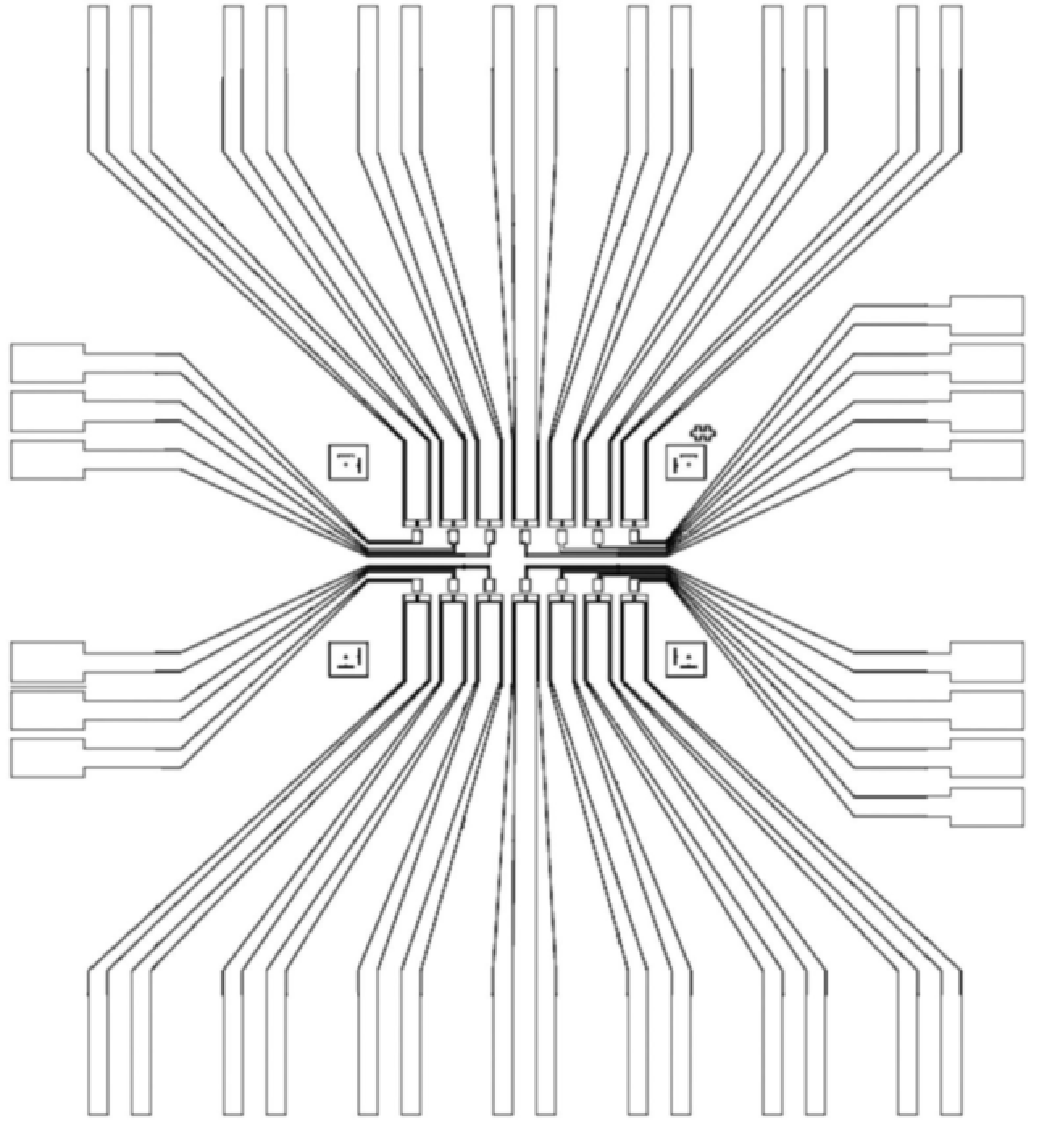
\includegraphics[width=5cm]{Images/pdf/photomask.pdf}
  \caption{Used photomask for fabricated OECT gold electrodes.}
  \label{fig:mask}
\end{figure}

\section{Experimental Procedure}

All fabrication steps were performed under standard cleanroom conditions.
\subsection{Preparation of Films} \label{subsec:films}
\paragraph{Dynamic spin-coating of p(g3T2-T).} In contrast to the approach described in reference \cite{tanTuningOrganicElectrochemical2022}, which employed drop-casting for the deposition of undoped and doped p(g3T2-T) films, our objective is to enable photolithography and facilitate a miniaturization process. To achieve this, uniform films are needed. The BioSens group members at IAPP had previously established dynamic spin-coating method due to the high volatility of p(g3T2-T) solvent, chloroform. Substrates were cleaned through sequential steps of ultrasonic bath in acetone for 15 minutes, IPA rinse, N$_{2}$ drying, and 5 minutes of O$_{2}$ plasma etching (0.3 mbar). Then, 70$\mu$L of 10 mg/mL of p(g3T2-T) mixed at 60$^{\circ}$C for 20 minutes, was applied using dynamic spin-coating at 3000 RPM for 60s, yielding approximately 70nm thick films. The samples were then dried at 80$^{\circ}$C.

\begin{figure}[ht]
  \centering
  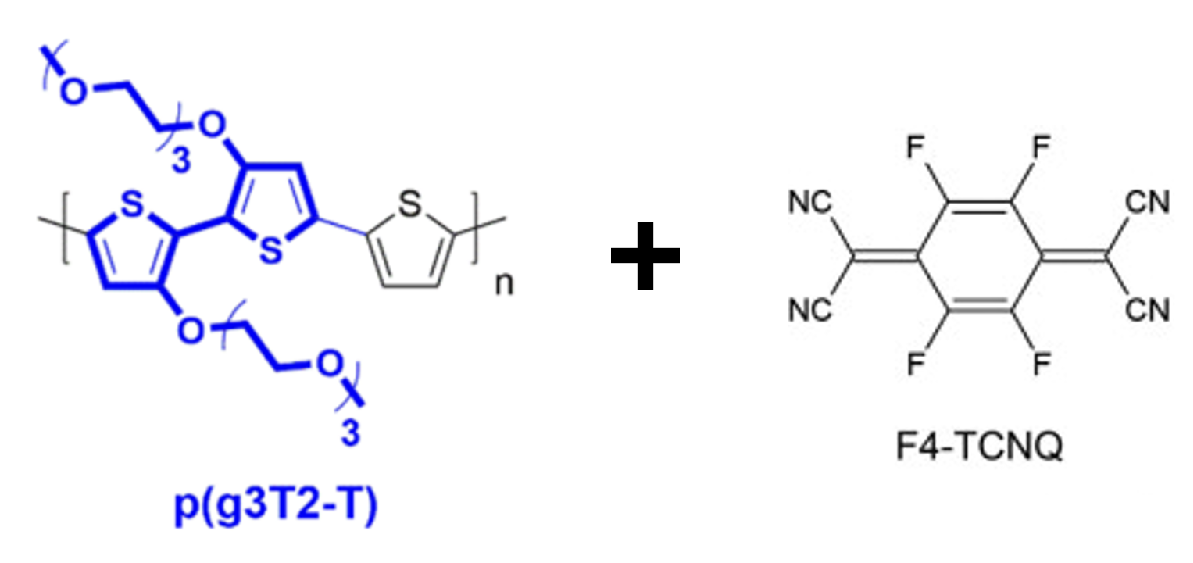
\includegraphics[width=8cm]{Images/pdf/doping_formulas1.pdf}
  \caption{Chemical structures of the repeat units of p(g3T2-T) and F$_{4}$TCNQ dopant.}
  \label{fig:dop1}
\end{figure}

\paragraph{Dynamic spin-coating of F$_{4}$TCNQ dopant.}Different doping levels of p(g3T2-T) were achieved by dynamic spin-coating 140$\mu$L of dopants at different concentrations (5, 10 and 20 mg/mL, as seen in Figure \ref{fig:coating}), previously mixed in acetronitrile at $60^{\circ}$C for 20 minutes. The samples were then dried at 80$^{\circ}$C.

\begin{figure}[ht]
  \centering
  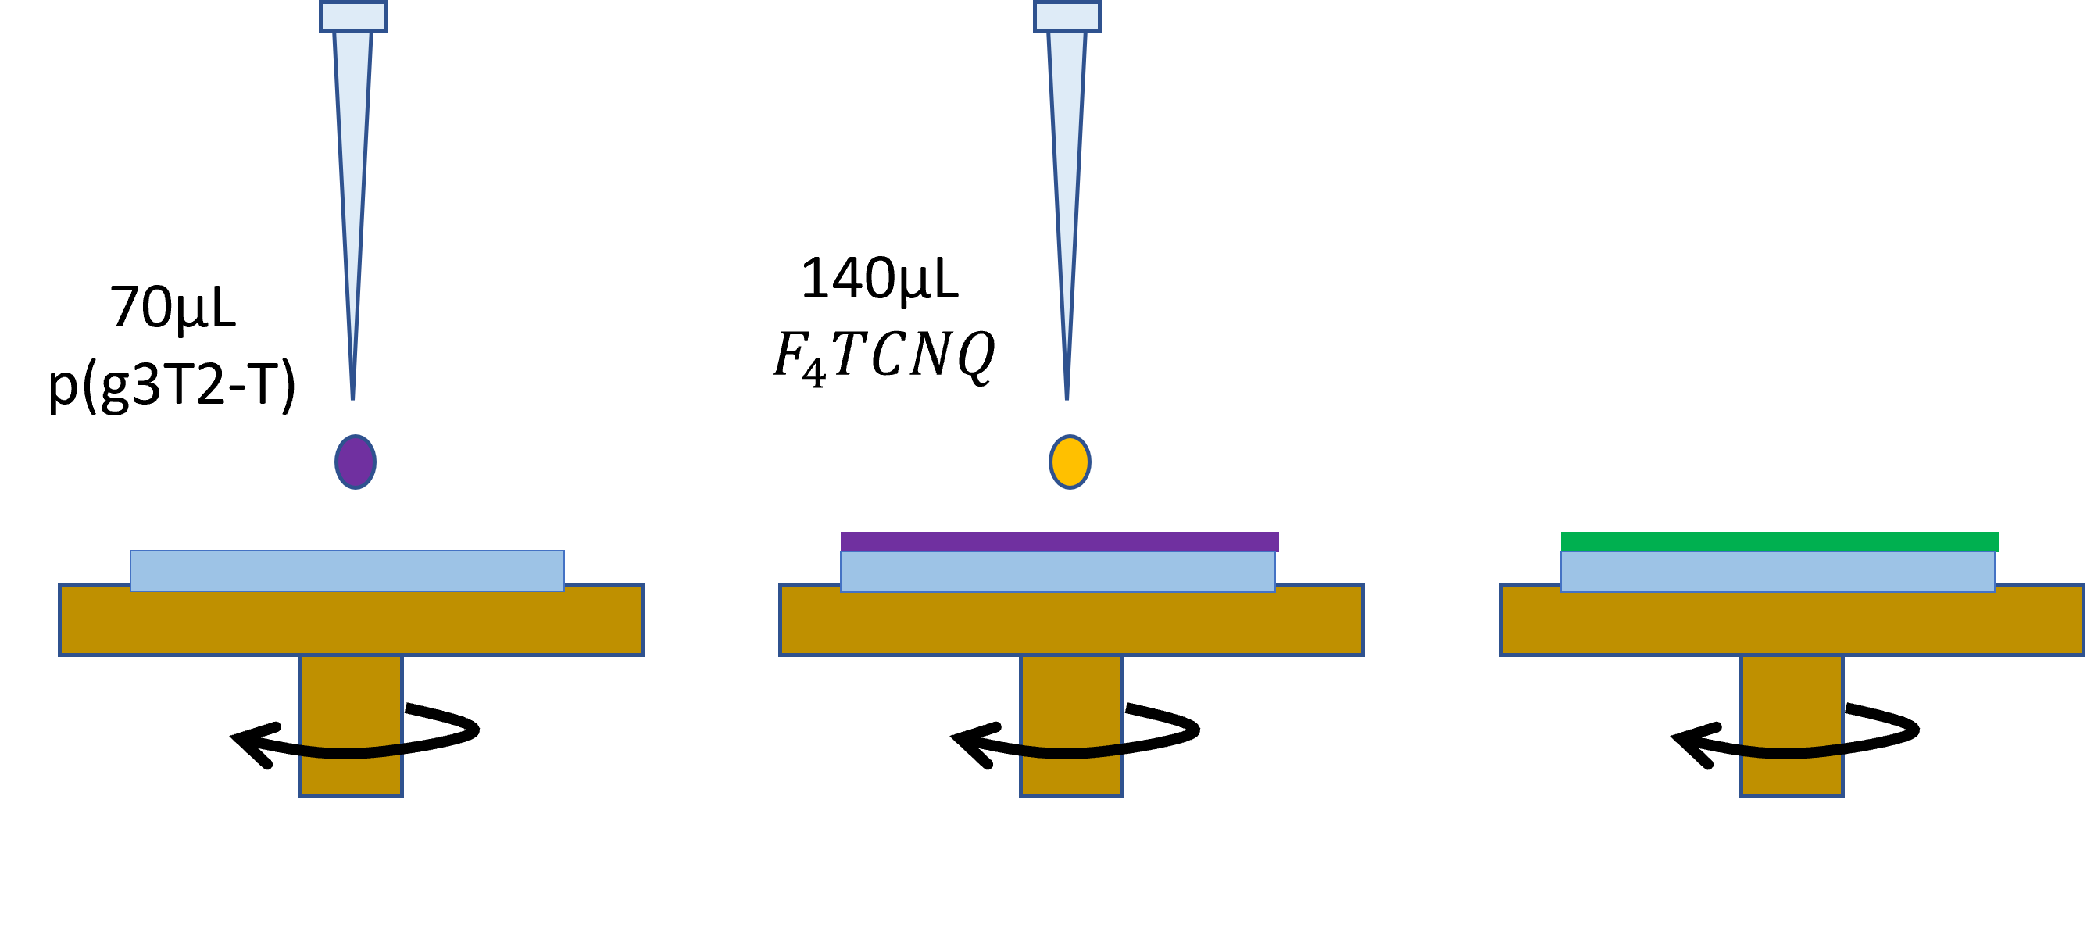
\includegraphics[width=10cm]{Images/pdf/spin_coating.pdf}
  \caption{Dynamic spin-coating process to obtain undoped and doped films of p(g3T2-T)).}
  \label{fig:coating}
\end{figure}

\subsection{Doping Characterization of Films}

\paragraph{Profilometer.}The films were scratched 4 times to remove part of material, and measure the cavity depth to obtain the film thickness.

\paragraph{Four-point probe.} A four-point probe was used to calculate the relation between induced voltage in inner probes and input current between outer probes. Then sheet resistance and resistivity were calculated using the Van Der Pauw method, following reference \cite{resist}, via equations:

\begin{equation}\label{eq:rs}
	R_{S} = \frac{\pi}{ln(2)}R = 4,53 R \quad [\Omega/sq],
\end{equation}

where R is the resistance measured with the four-point probe setup, and

\begin{equation}\label{eq:resist}
	\rho = R_{s}t \quad [\Omega.cm],
\end{equation}
 
 where $t$ is the thickness of the film.

\paragraph{UV-Vis-NIR Spectroscopy.}After the preparation of the films onto quartz substrates, transmittance (T) and reflectance (R) was measured using the UV-Vis-NIR Spectrometer in the range of 285 to 1600 nm. Then, absorption (A) was calculated via

\begin{equation}\label{eq:abs}
	A = 1 - T - R,
\end{equation}

and normalized with respect to the incoming light \cite{uvvis}. Additional measurements were taken, after some days of storage under ambient conditions to check its stability in air.

\paragraph{Ultraviolet Photoelectron Spectroscopy.}After the preparation of the films, %(air exposure) 
the energy of the highest occupied molecular orbital cutoff (E$_{HOMO}$) and the high binding energy cutoff E$_{HBEC}$ was measuring using UPS. The pressure in the chamber during measurements was about 5$\cdot$10$^{-9}$ mbar, while the base pressure is in the range of 10$\cdot$10$^{-10}$ mbar. The workfunction (WF) and ionization energy (IE) are calculated by using the following equations:

\begin{equation}\label{eq:wf}
	WF = h\nu - E_{HBEC} \quad [eV],
\end{equation}

\begin{equation}\label{eq:ie}
	IE = h\nu - (E_{HBEC}-E_{HOMO}) \quad [eV],
\end{equation}

where $h\nu = 21.22 eV$, the main He I excitation line of the Helium plasma discharge lamp \cite{buchholtzDopingPropertiesNovel2021}. 
 
%\subsection{Roughness characterization of films} 

\subsection{Doping in Organic Electrochemical Transistors} \label{subsec:oect}

\subsubsection{Influence of Doping on OECT Channel} \label{subsec:channel}

Photolithographically patterned substrates with gold contacts for source, drain and gate were obtained using mask layout illustrated in Figure \ref{fig:mask}. The steps outlined in references \cite{weissbachPhotopatternableSolidElectrolyte2022} and \cite{bongartzOrganicElectrochemicalTransistors2021} were followed, which is also represented in Figure \ref{fig:aupat}.

\begin{figure}[ht]
	\centering
	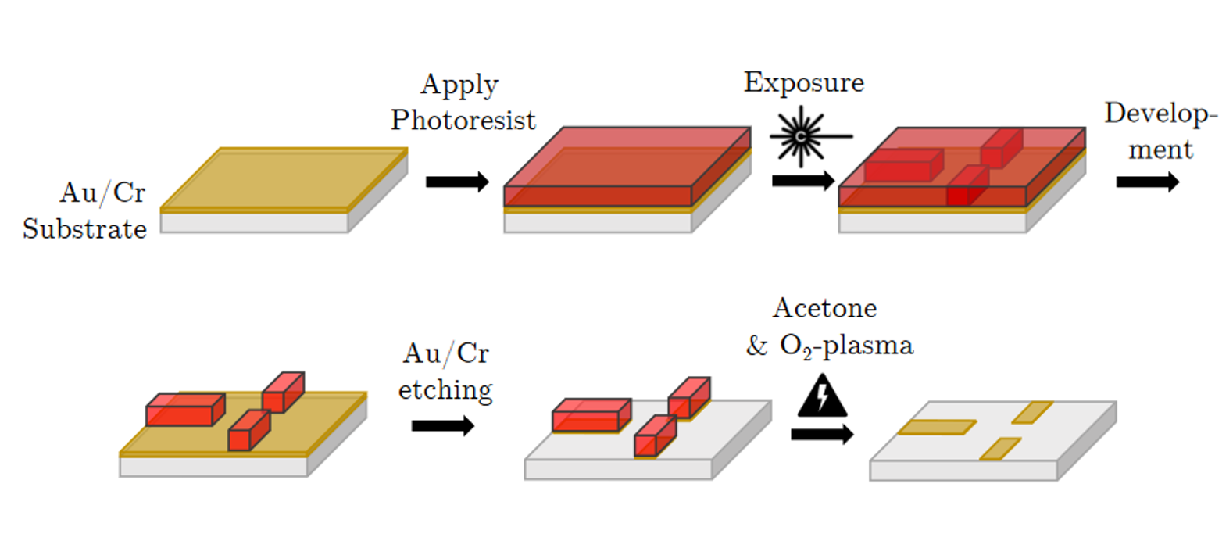
\includegraphics[width=12cm]{Images/pdf/Au-patterning.pdf}
	\caption[Visualization of the workflow for Au-contacts patterning.]{Visualization of the workflow for Au-contacts patterning. Image modified based on reference \cite{bongartzOrganicElectrochemicalTransistors2021}.}
	\label{fig:aupat}
\end{figure}

Then p(g3T2-T) films were deposited following the procedure described in the previous section. The patterning of doped-p(g3T2-T) channel adopted a procedure similar to the one described in references \cite{weissbachPhotopatternableSolidElectrolyte2022}\cite{bongartzOrganicElectrochemicalTransistors2021}, which involves the use of PEDOT:PSS. However, some modifications in the exposure and developing times were made. In contrast, the patterning of undoped-p(g3T2-T) samples, required a different protocol. A sacrificial layer is introduced to ensure proper cross-linking with photoresist. Both processes are detailed in the following:

\paragraph{Patterning undoped p(g3T2-T).}Patterning of the p(g3T2-T) was achieved with photolithography, as shown in Figure \ref{fig:undopedpat}. First, a fluoropolymer Sacrificial Layer 1 (SL1) was spin-coated at 6000 RPM for 60 s, followed by a baking step for 180 s at $113^{\circ}$C. Before the deposition of photoresist, a O$_{2}$ plasma cleaning step was applied for 60 s to promote adhesion. Then, NLOF 2020 photoresist was spin-coated at 3000 RPM for 60 s and baked for another 60 s at $113^{\circ}$C. Exposure of negative resist was performed for 12 s by shadowing all areas except the ones of interest. After post-baking for 60 s at $113^{\circ}$C, NLOF was developed by rinsing the sample in AZ MIF 726 for 20 s and wash off in DI water (carried out extra times if necessary). Next, SL1 was developed using HF 7300 developer for 45 s and spin rinsed at 3000 RPM (carried out extra times if necessary). Excess of p(g3T2-T) was removed by O$_{2}$-plasma etching for 180 s. The sample was placed in Orthogonal Stripper 900 overnight at room temperature, to complete the removal. Finally, ultrasonication in acetone was added for 15 min the next day. 

\begin{figure}[ht]
	\centering
	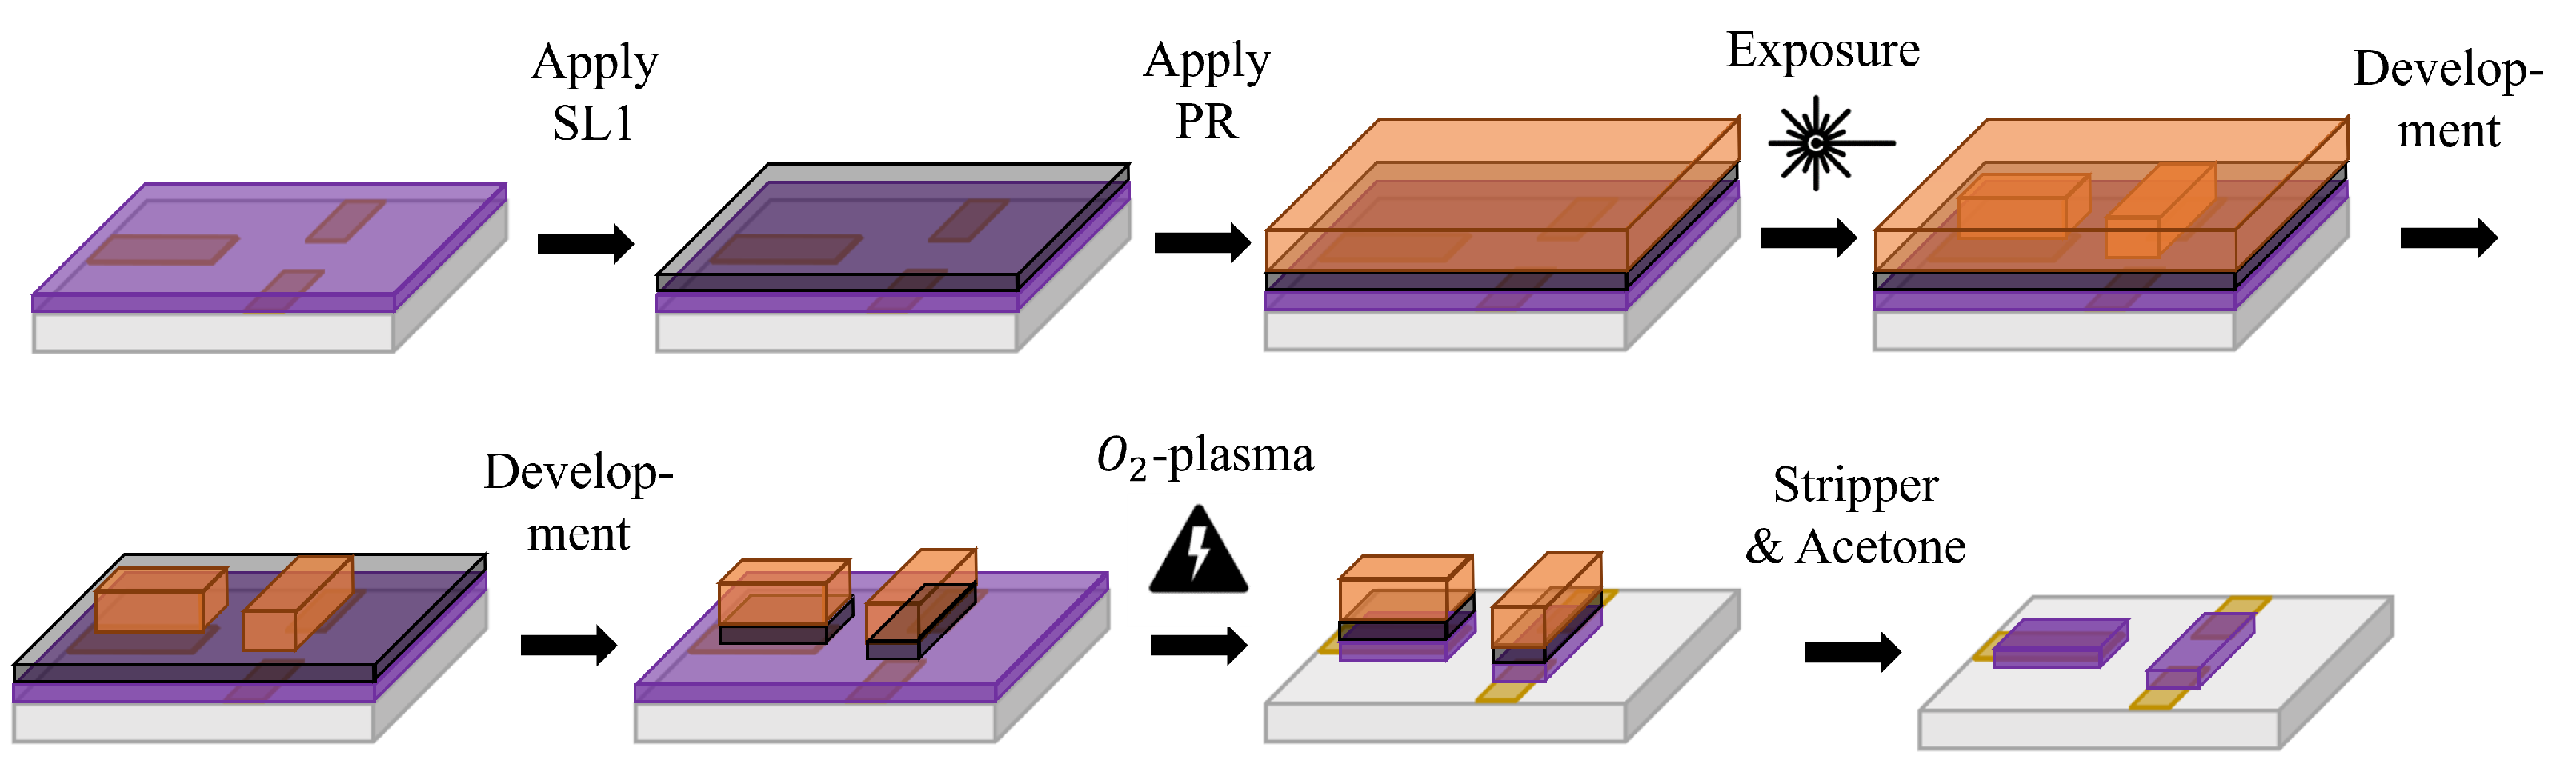
\includegraphics[width=12.5cm]{Images/pdf/undoped-patterning.pdf}
	\caption{Visualization of the workflow for patterning undoped p(g3T2-T).}
	\label{fig:undopedpat}
\end{figure}

\paragraph{Patterning doped p(g3T2-T).}Patterning of the doped p(g3T2-T) was achieved with photolithography, as shown in Figure \ref{fig:dopedpat}. First, the orthogonal photoresist OSCoR 4020 was spin coated at 3000 RPM for 60 s and baked for another 60 s at $103^{\circ}$C. Exposure of negative resist was performed for 20 s with shadowing all areas except the ones of interest, one extra cycle was added if using higher dopant concentration (10 mg/mL). After post-baking for 60 s at $103^{\circ}$C, OSCoR was developed using Orthogonal Developer 103a for 45 s and spin rinsed at 3000 RPM for 60 s (carried out extra times if necessary). Excess of doped-p(g3T2-T) was removed by O$_{2}$-plasma etching for 180 s. The sample was placed in Orthogonal Stripper 900 overnight at room temperature.

\begin{figure}[ht]
	\centering
	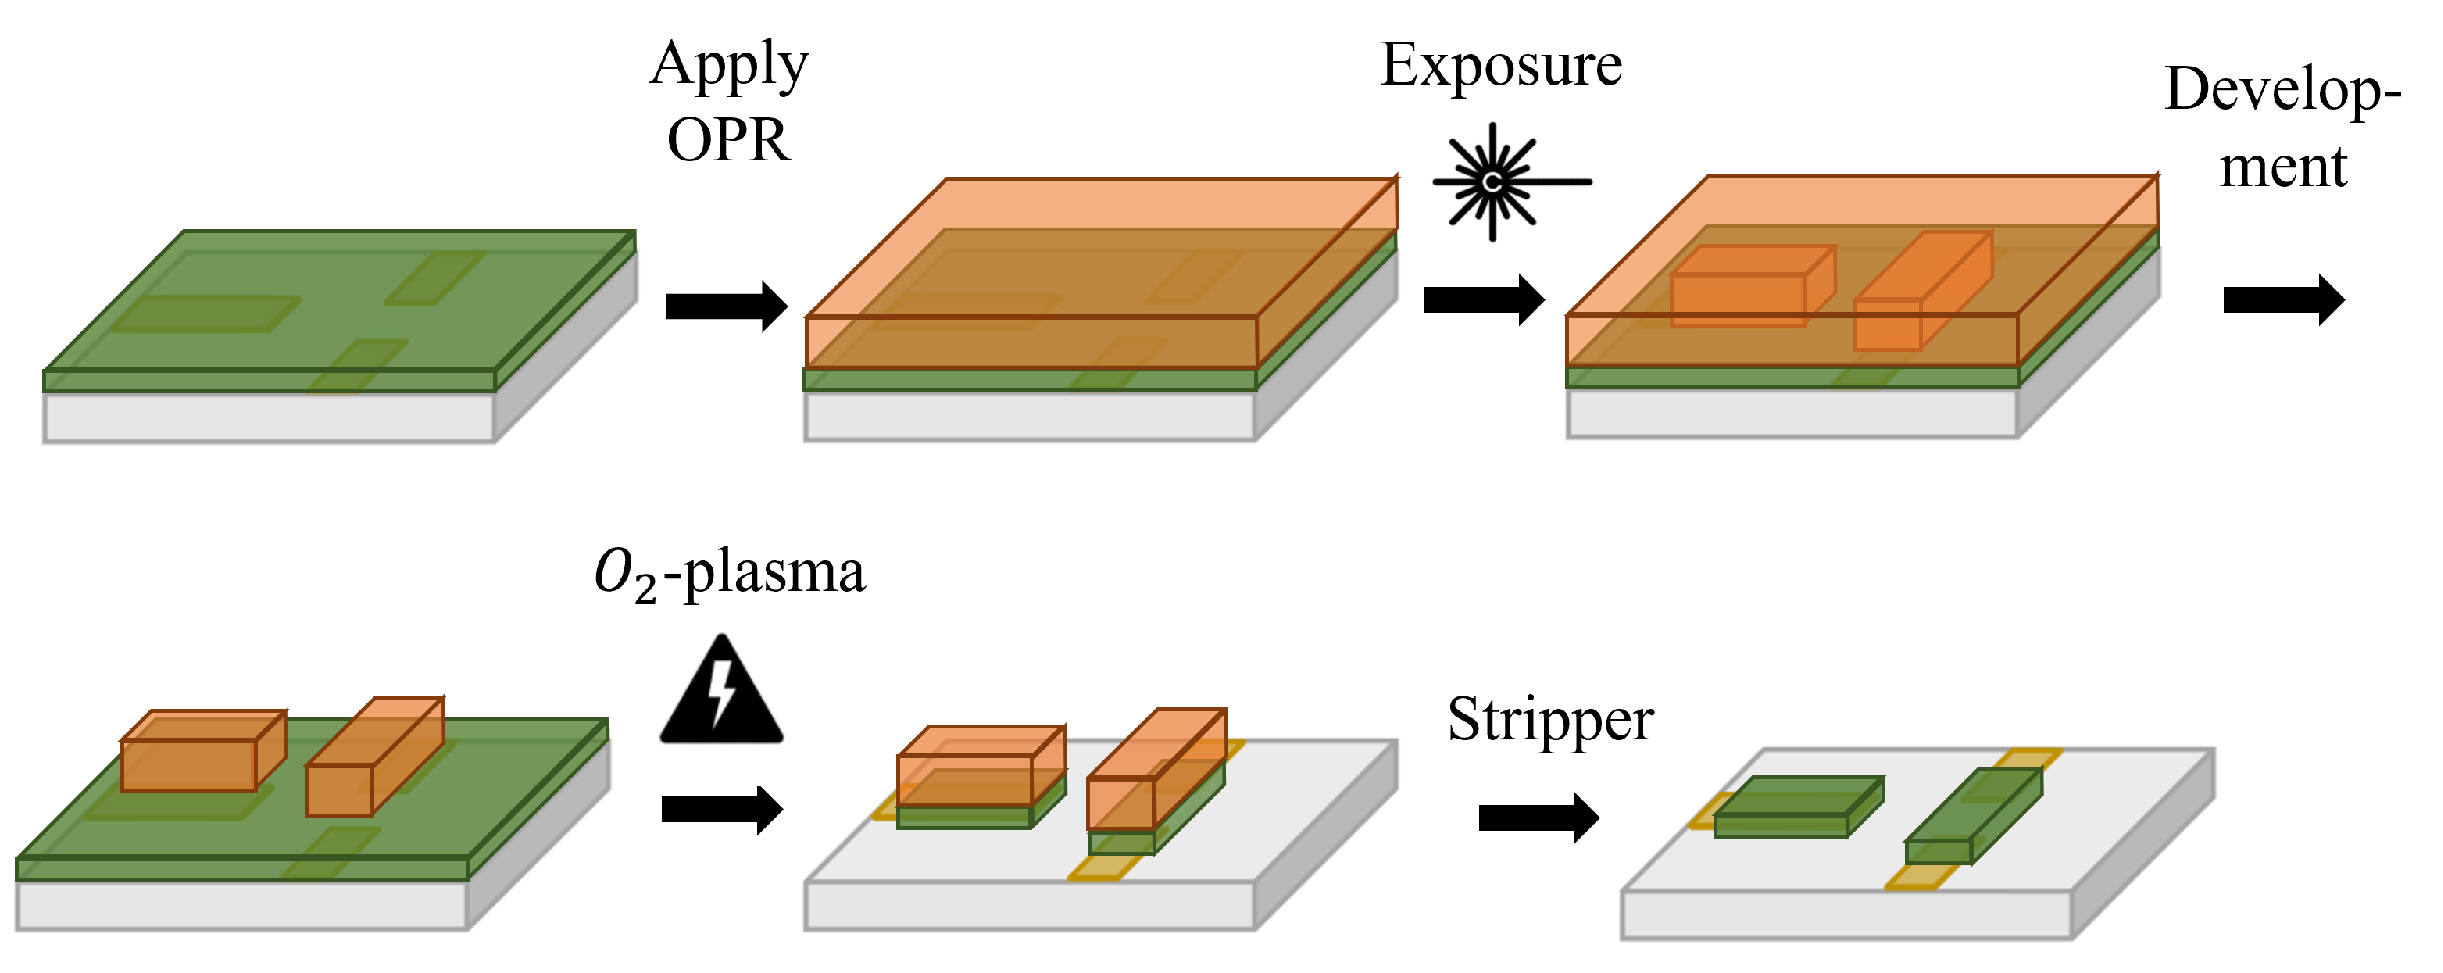
\includegraphics[width=10.5cm]{Images/pdf/doped-patterning.pdf}
	\caption{Visualization of the workflow for patterning doped p(g3T2-T).}
	\label{fig:dopedpat}
\end{figure}

\paragraph{OECT with undoped- and doped-p(g3T2-T) channel.} A solid-state electrolyte precursor was prepared according to the details provided in Table \ref{tab:sse}. Next, 20$\mu$L of this precursor were drop-casted to the patterned samples, both undoped and doped, covering all 14 devices in the sample. Finally, a Ag/AgCl pellet was installed and used as gate (Figure \ref{fig:biosetup}). Transfer characteristics were measured under ambient conditions with a V$_{GS}$ swept backwards from 1.0 V to -0.8 V. %at a scanning rate of 0.083 V/s.

\begin{table}[ht]
	\centering
	\caption{Composition of the solid-state electrolyte \cite{weissbachPhotopatternableSolidElectrolyte2022}.}
	\begin{tabular}{r c l} \hline
		Component   & Amount & Function \\ \hline
		H$_{2}$O	& 1.0 mL & dilution \\ 
		$[$EMIM$][$EtSO$_{4}]$   & 1.5 mL & ionic liquid \\ 
		MBBAm   & 20 mg & crosslinker \\ 
		NIPAm   & 750 mg & monomer \\ 
		HHPAA   & 200 mg & photoinitiator \\
		EG	& 1.5 mL	& increase viscosity, ensures good print \\ 
		Triton & 1 drop & surfactant, ensures good print \\  \hline
	\end{tabular}
	\label{tab:sse}
\end{table}

\begin{figure}[!ht]
	\centering
	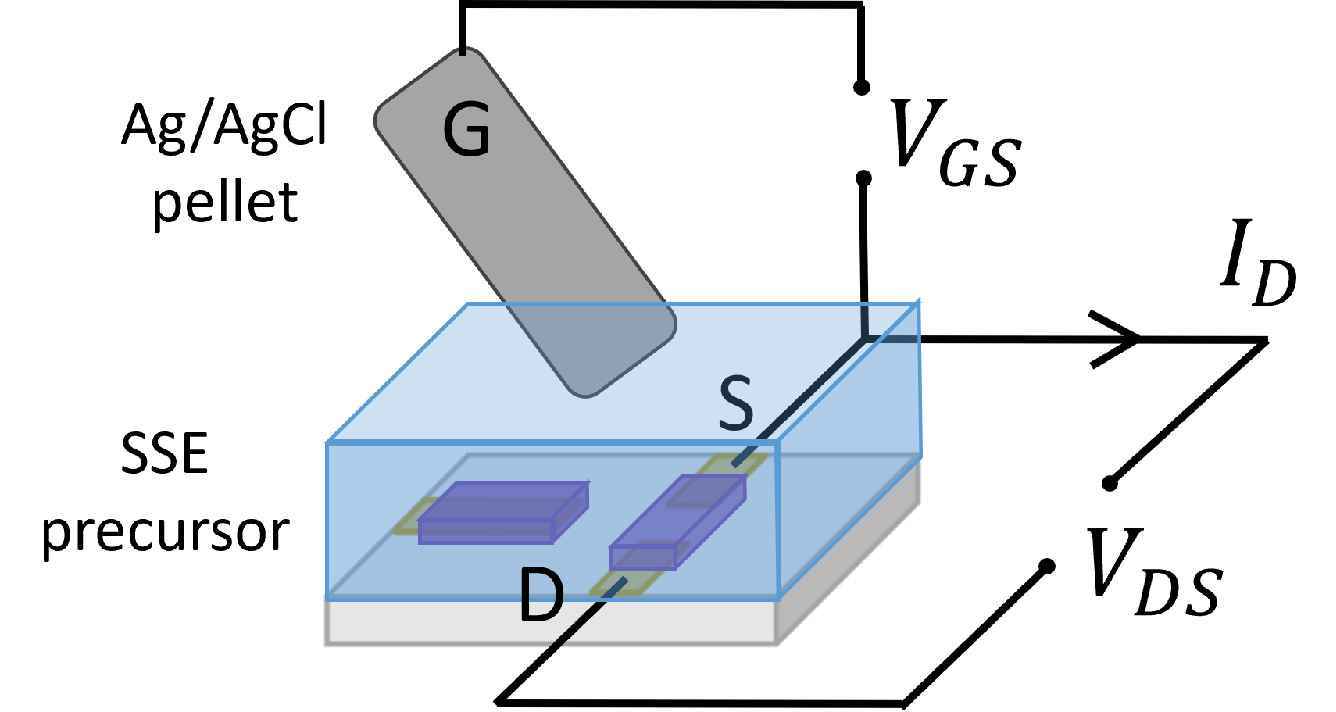
\includegraphics[width=5.5cm]{Images/pdf/bioprobe_setup.pdf}
	\caption{Representation of experimental setup for measuring threshold voltage shift of a single OECT under ambient conditions. Scheme is not drawn to scale.}
	\label{fig:biosetup}
\end{figure}

\newpage
%\subsubsection{Stability on Air of p(g3T2-T)}
\subsubsection{Stability of Undoped and Doped p(g3T2-T)}
In this subsection, stability tests were conducted on both undoped and doped p(g3T2-T) samples. These samples were doped with F$_{6}$TCNNQ, following same procedure described in subsection \ref{subsec:films}. %The channel conductivity was measured %at various stages of the photolithography process, 
%before and after patterning and after contact with SSE %
%while a fixed biased drain-source voltage was maintained, under N$_{2}$ and ambient conditions. %, upon spin-coating, patterning, i) upon dropcast of solid-state electrolyte precursor, and after exposure, ii) after photopatterned solid-state electrolyte, and finally

\begin{figure}[ht]
  \centering
  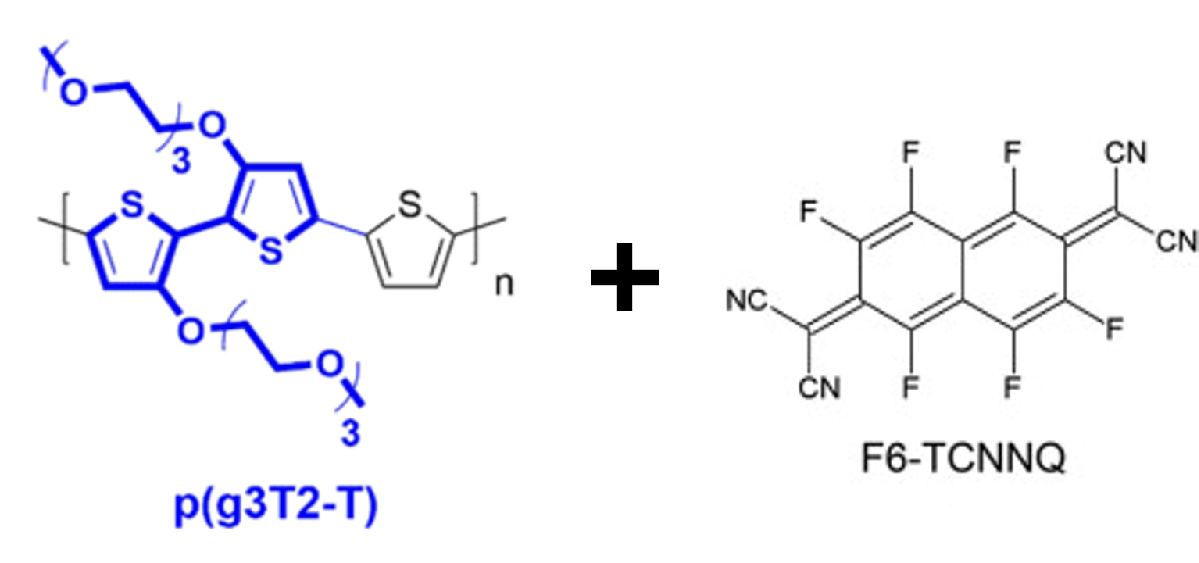
\includegraphics[width=7cm]{Images/pdf/doping_formulas2.pdf}
  \caption{Chemical structures of the repeat units of p(g3T2-T) and F$_{6}$TCNNQ dopant.}
  \label{fig:dop2}
\end{figure}

\paragraph{Channel conductivity measurements.}The channel conductivity of an undoped-p(g3T2-T) device was measured in N$_{2}$ then ambient conditions immediately after spin-coating onto substrate with patterned gold contacts. The channel conductivities of both doped and undoped devices were monitored after patterning process (as described in previous section) for two hours under N$_{2}$ environment, and for 1h30 under ambient environment. Finally, they were again monitored upon drop-casting solid-state electrolyte precursor.
%Undoped-p(g3T2-T) sample was measured in N$_{2}$ then ambient conditions immediately after spin-coating onto substrate with patterned gold contacts. Then, sample was measured after patterning process (as described in previous section). Finally, upon drop-casting solid-state electrolyte precursor. The doped-p(g3T2-T) channel was measured after patterning and upon drop-casting solid-state electrolyte precursor.

\paragraph{Transfer characteristics.} Transfer characteristics were measured at different $V_{DS}$ (-0.5, -0.3, -0.1 V) of the undoped p(g3T2-T) device using a Ag/AgCl pellet as gate under environmental conditions, immediately after finalizing the process described above.

\subsubsection{Counteracting Oxidation of Undoped p(g3T2-T) by Electrochemical De-doping}

\paragraph{Channel conductivity measurements.}Undoped p(g3T2-T) samples onto patterned-gold-contacts substrates were prepared. The solid-state electrolyte precursor was drop-casted onto the 14 devices, one device source-drain was negatively-biased and applied a positive gate voltage (+1 V). Channel conductivity was monitored. %Finally, other devices on the sample were measured to detect any effect of the process.

\paragraph{Transfer characteristics.}Transfer characteristics were measured at $V_{DS}$ of -0.1 using the OMIEC gate under N$_{2}$ environment, immediately after process described above. Other measurements were performed after UV light exposure, and in ambient conditions using a Ag/AgCl pellet gate.
 
%\paragraph{By heating.}An undoped-p(g3T2-T) solid-OECT, whose fabrication will be described in the following subsection \ref{subsec:solidOECT}, was exposed to ambient conditions, devices were clearly oxidized. The sample was placed on a hot plate at 120$^{\circ}$C, brought back to glovebox, and measured the following day.  %\cite{weissbachPhotopatternableSolidElectrolyte2022}.
%% alcohol rinse

\subsection{Fabrication of Solid Organic Electrochemical Transistors} \label{subsec:soect}

\subsubsection{Solid-OECTs using Undoped-p(g3T2-T)} \label{subsec:solidOECT}
After following the patterning steps for undoped-p(g3T2-T) from Subsection \ref{subsec:channel}. Three different methods of applying the solid-state electrolyte precursor were tested. Then, transfer characteristics were measured at a constant V$_{DS}$ of -0.1V, and a  V$_{GS}$ swept backwards from 1.0 V to 1.0 V at a scanning rate of 0.083 V/s. Cyclic voltammetry and electrochemical impedance spectroscopy were performed by short-circuiting source and drain to probe between channel and gate. Parameters were fixed as described in Section \ref{param}, and measurements were taken one day after the fabrication.

\paragraph{Application of adhesion promoter.}An adhesion promoter, consisting of reactants detailed in Table \ref{tab:adprom}, was applied to the substrate. The sample was placed in a Petri dish at 50$^{\circ}$C and covered for 20 min. Subsequently, it was thoroughly rinse with ethanol and dried on a hot plate at 100$^{\circ}$C for a minimum of 10 min. The composition and application steps of adhesion promoter was previously established by Biosens group members at IAPP. 

\begin{table}[ht]
	\centering
	\caption{Composition of adhesion promoter.}
	\begin{tabular}{r r} \hline
		Component   & Amount \\ \hline
		SilaneA174	& 30 $\mu$L \\ 
		Etanol   & 3mL \\ 
		Acetic acid   & 60 $\mu$L \\ \hline
	\end{tabular}
	\label{tab:adprom}
\end{table}

\paragraph{OECT with drop-casted Solid-State Electrolyte.}Solid-state electrolyte precursor was drop-casted and then exposed for 2 cycles of 60 s in a mask aligner, as shown in Figure \ref{fig:undopedsse}a. No adhesion promoter was applied in this sample.

\paragraph{OECT with photopatternable Solid-State Electrolyte.}After the application of the adhesion promoter, the solid-state electrolyte precursor was drop-casted onto the sample, followed by the placement of a Teflon foil to prevent contact with the mask, which would shadow all areas except the ones of interest in the negative resist. The sample was then exposed for 2 cycles of 60 s in a mask aligner. Removal of excess, non-cross-linked precursor was careful blown off with a N$_{2}$ gun, as shown in Figure \ref{fig:undopedsse}b,  following references \cite{weissbachPhotopatternableSolidElectrolyte2022}\cite{bongartzOrganicElectrochemicalTransistors2021}.

\paragraph{OECT with inkjet-printed Solid-State Electrolyte.}After the application of the adhesion promoter, the solid-state-electrolyte precursor was ink-jet printed and expose for 2 cycles of 60 s in mask aligner, as illustrated in Figure \ref{fig:undopedsse}c. Parameters and procedure for ink-jet printing was previously established by members of BioSens group at IAPP \cite{tsengThresholdVoltageControl2023}. 

\begin{figure}[!ht]
	\centering
	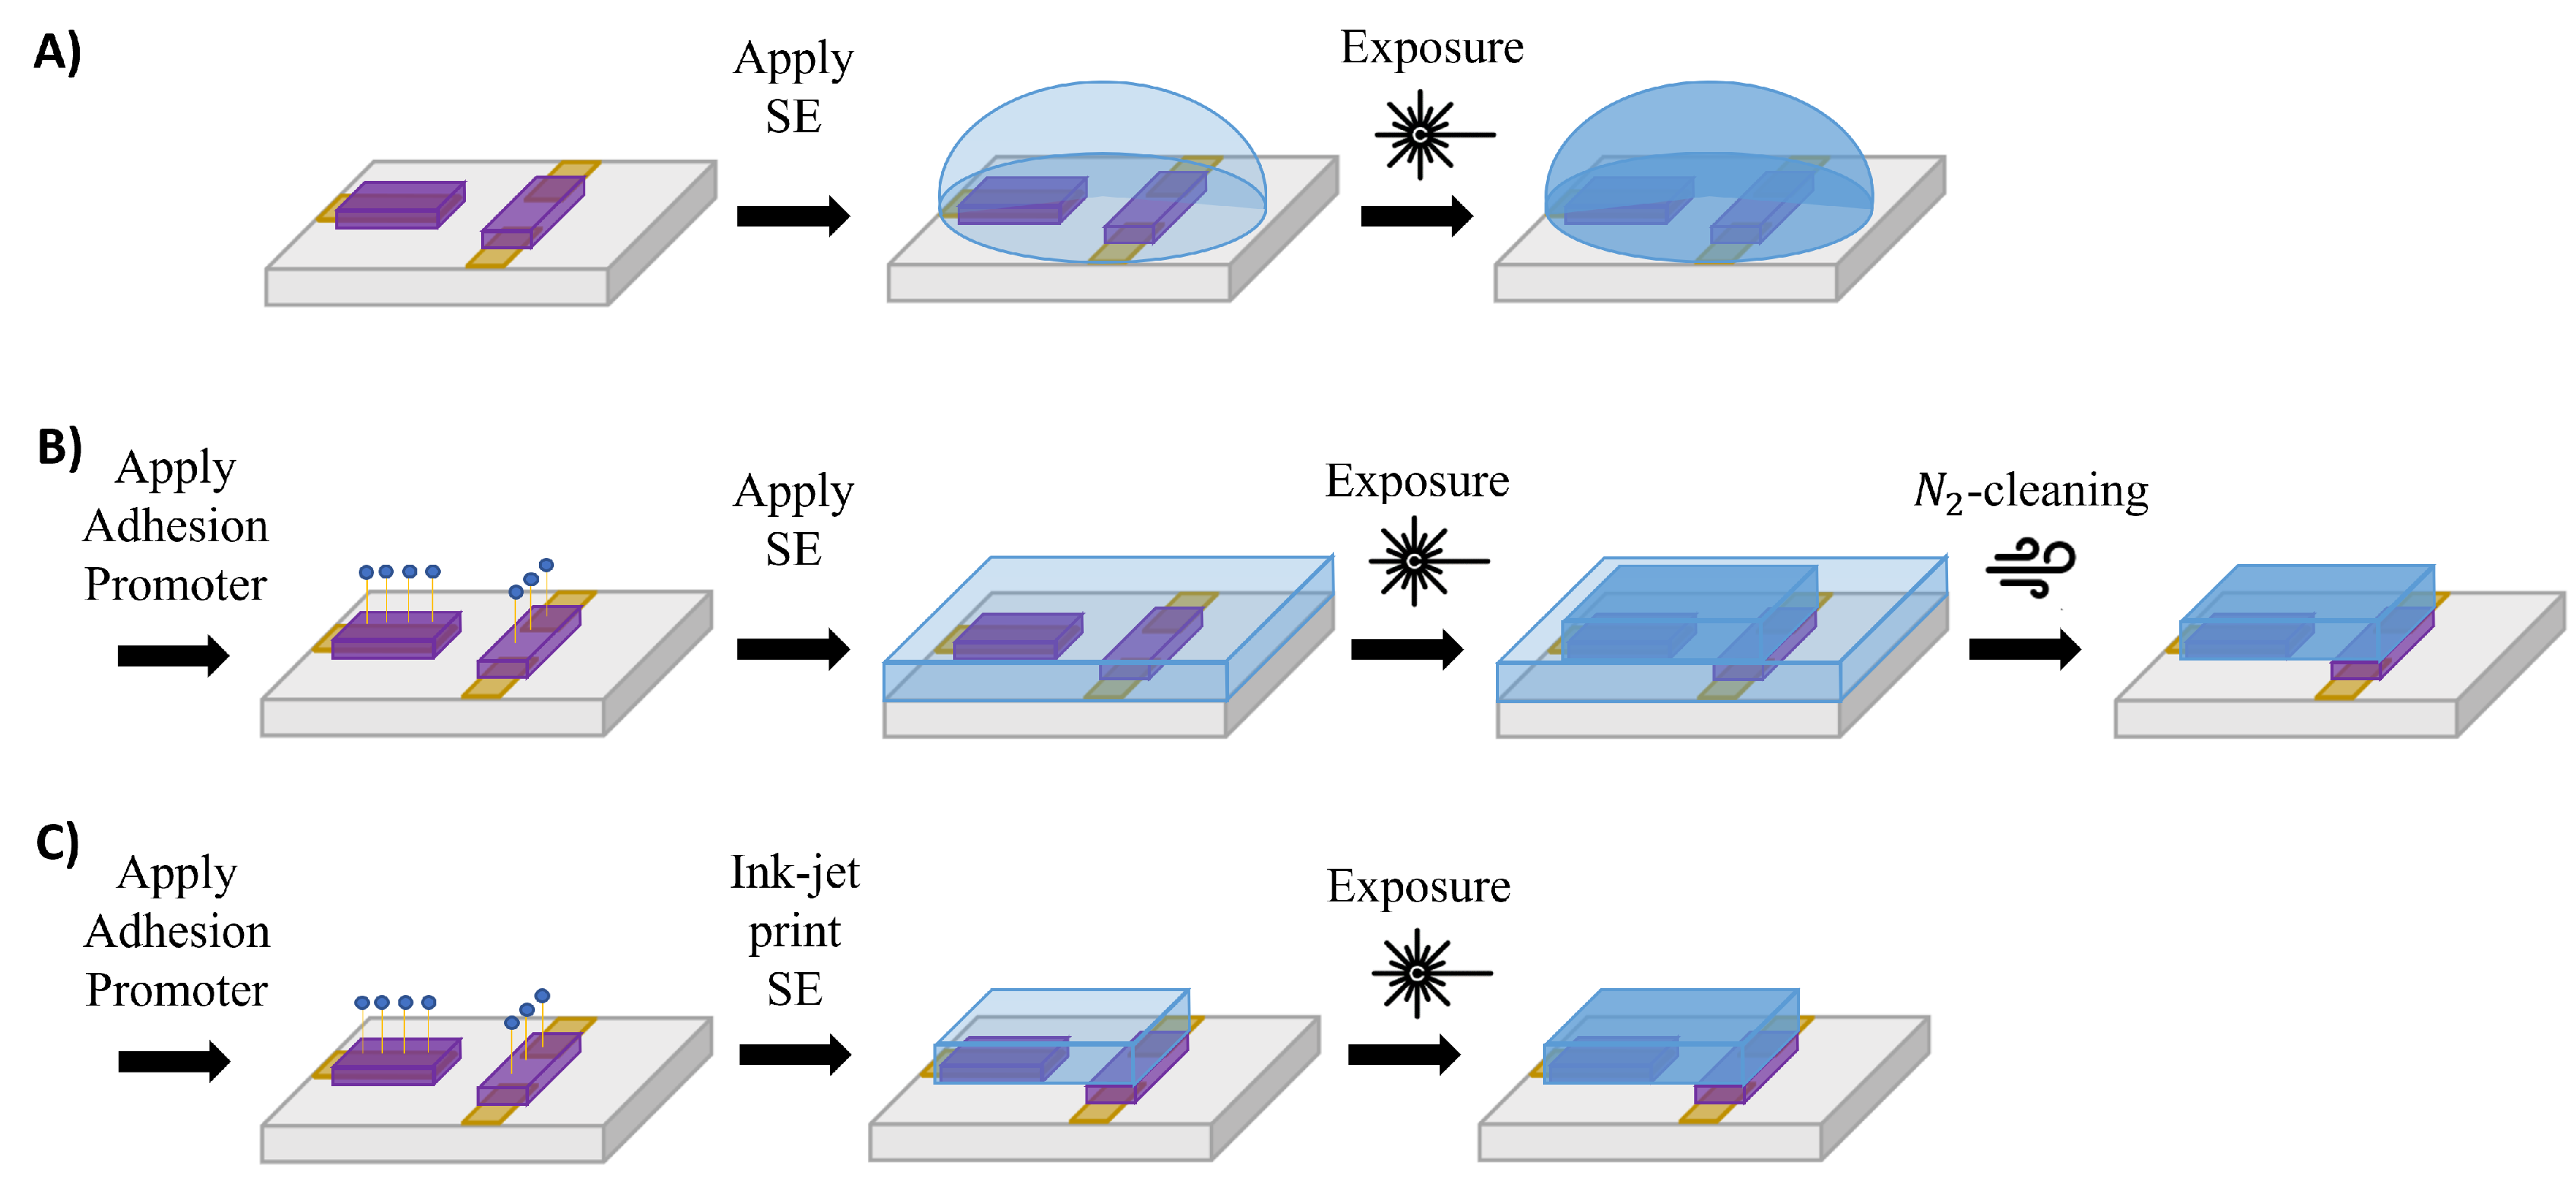
\includegraphics[width=12cm]{Images/pdf/undoped-sse.pdf}
	\caption[Solid-OECT fabrication with undoped p(g3T2-T)]{Visualization of the workflow for solid-OECT fabrication with undoped p(g3T2-T) by A) drop-casting SSE, B) photopatterning SSE, C) ink-jet printing SSE.}
	\label{fig:undopedsse}
\end{figure}

\subsubsection{Solid-OECTs using Doped-p(g3T2-T)}

\paragraph{OECT with inkjet-printed Solid-State Electrolyte.}After the deposition of films and dopant (F$_{6}$TCNNQ), films were stored in glovebox over the weekend to let dopants soak and dry. Then, the patterning steps for doped-p(g3T2-T) from Subsection \ref{subsec:channel} were followed with no extra cycles in exposure times. Solid-state electrolyte precursor was ink-jet printed as described in the previous subsection. Then, transfer characteristics were measured at a constant V$_{DS}$ of -0.1V, and  a  V$_{GS}$ swept backwards from 1.0 V to 1.0 V at a scanning rate of 0.083 V/s. Cyclic voltammetry and electrochemical impedance spectroscopy were performed by short-circuiting source and drain to probe between channel and gate. Parameters were fixed as described in Section \ref{param}, and measurements were taken one day after the fabrication.

\begin{figure}[!t]
	\centering
	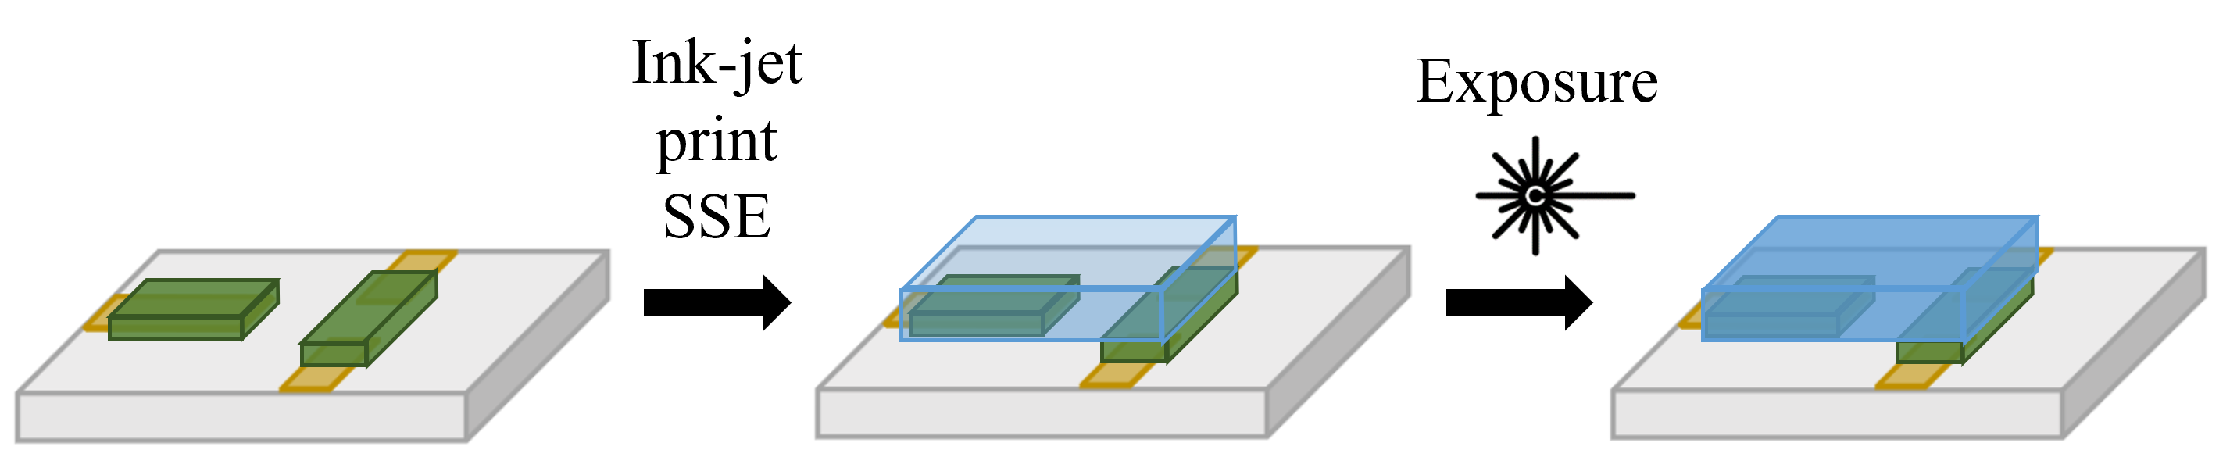
\includegraphics[width=9cm]{Images/pdf/doped-sse.pdf}
	\caption[Solid-OECT fabrication with doped p(g3T2-T)]{Visualization of the workflow for solid-OECT fabrication with doped p(g3T2-T) by ink-jet printing SSE.}
	\label{fig:dopedsse}
\end{figure}

%%% Local Variables: 
%%% mode: latex
%%% TeX-master: "thesis"
%%% End: 

\chapter{Results and Discussion}
\label{cha:3}

\section{Doping Characterization}

Upon increase of the dopant concentration that is deposited and bake on top of the p(g3T2-T) film, the reflection hue, as observed in Figure \ref{fig:color} shift towards more yellowish colors.

\begin{figure}[ht]
  \centering
  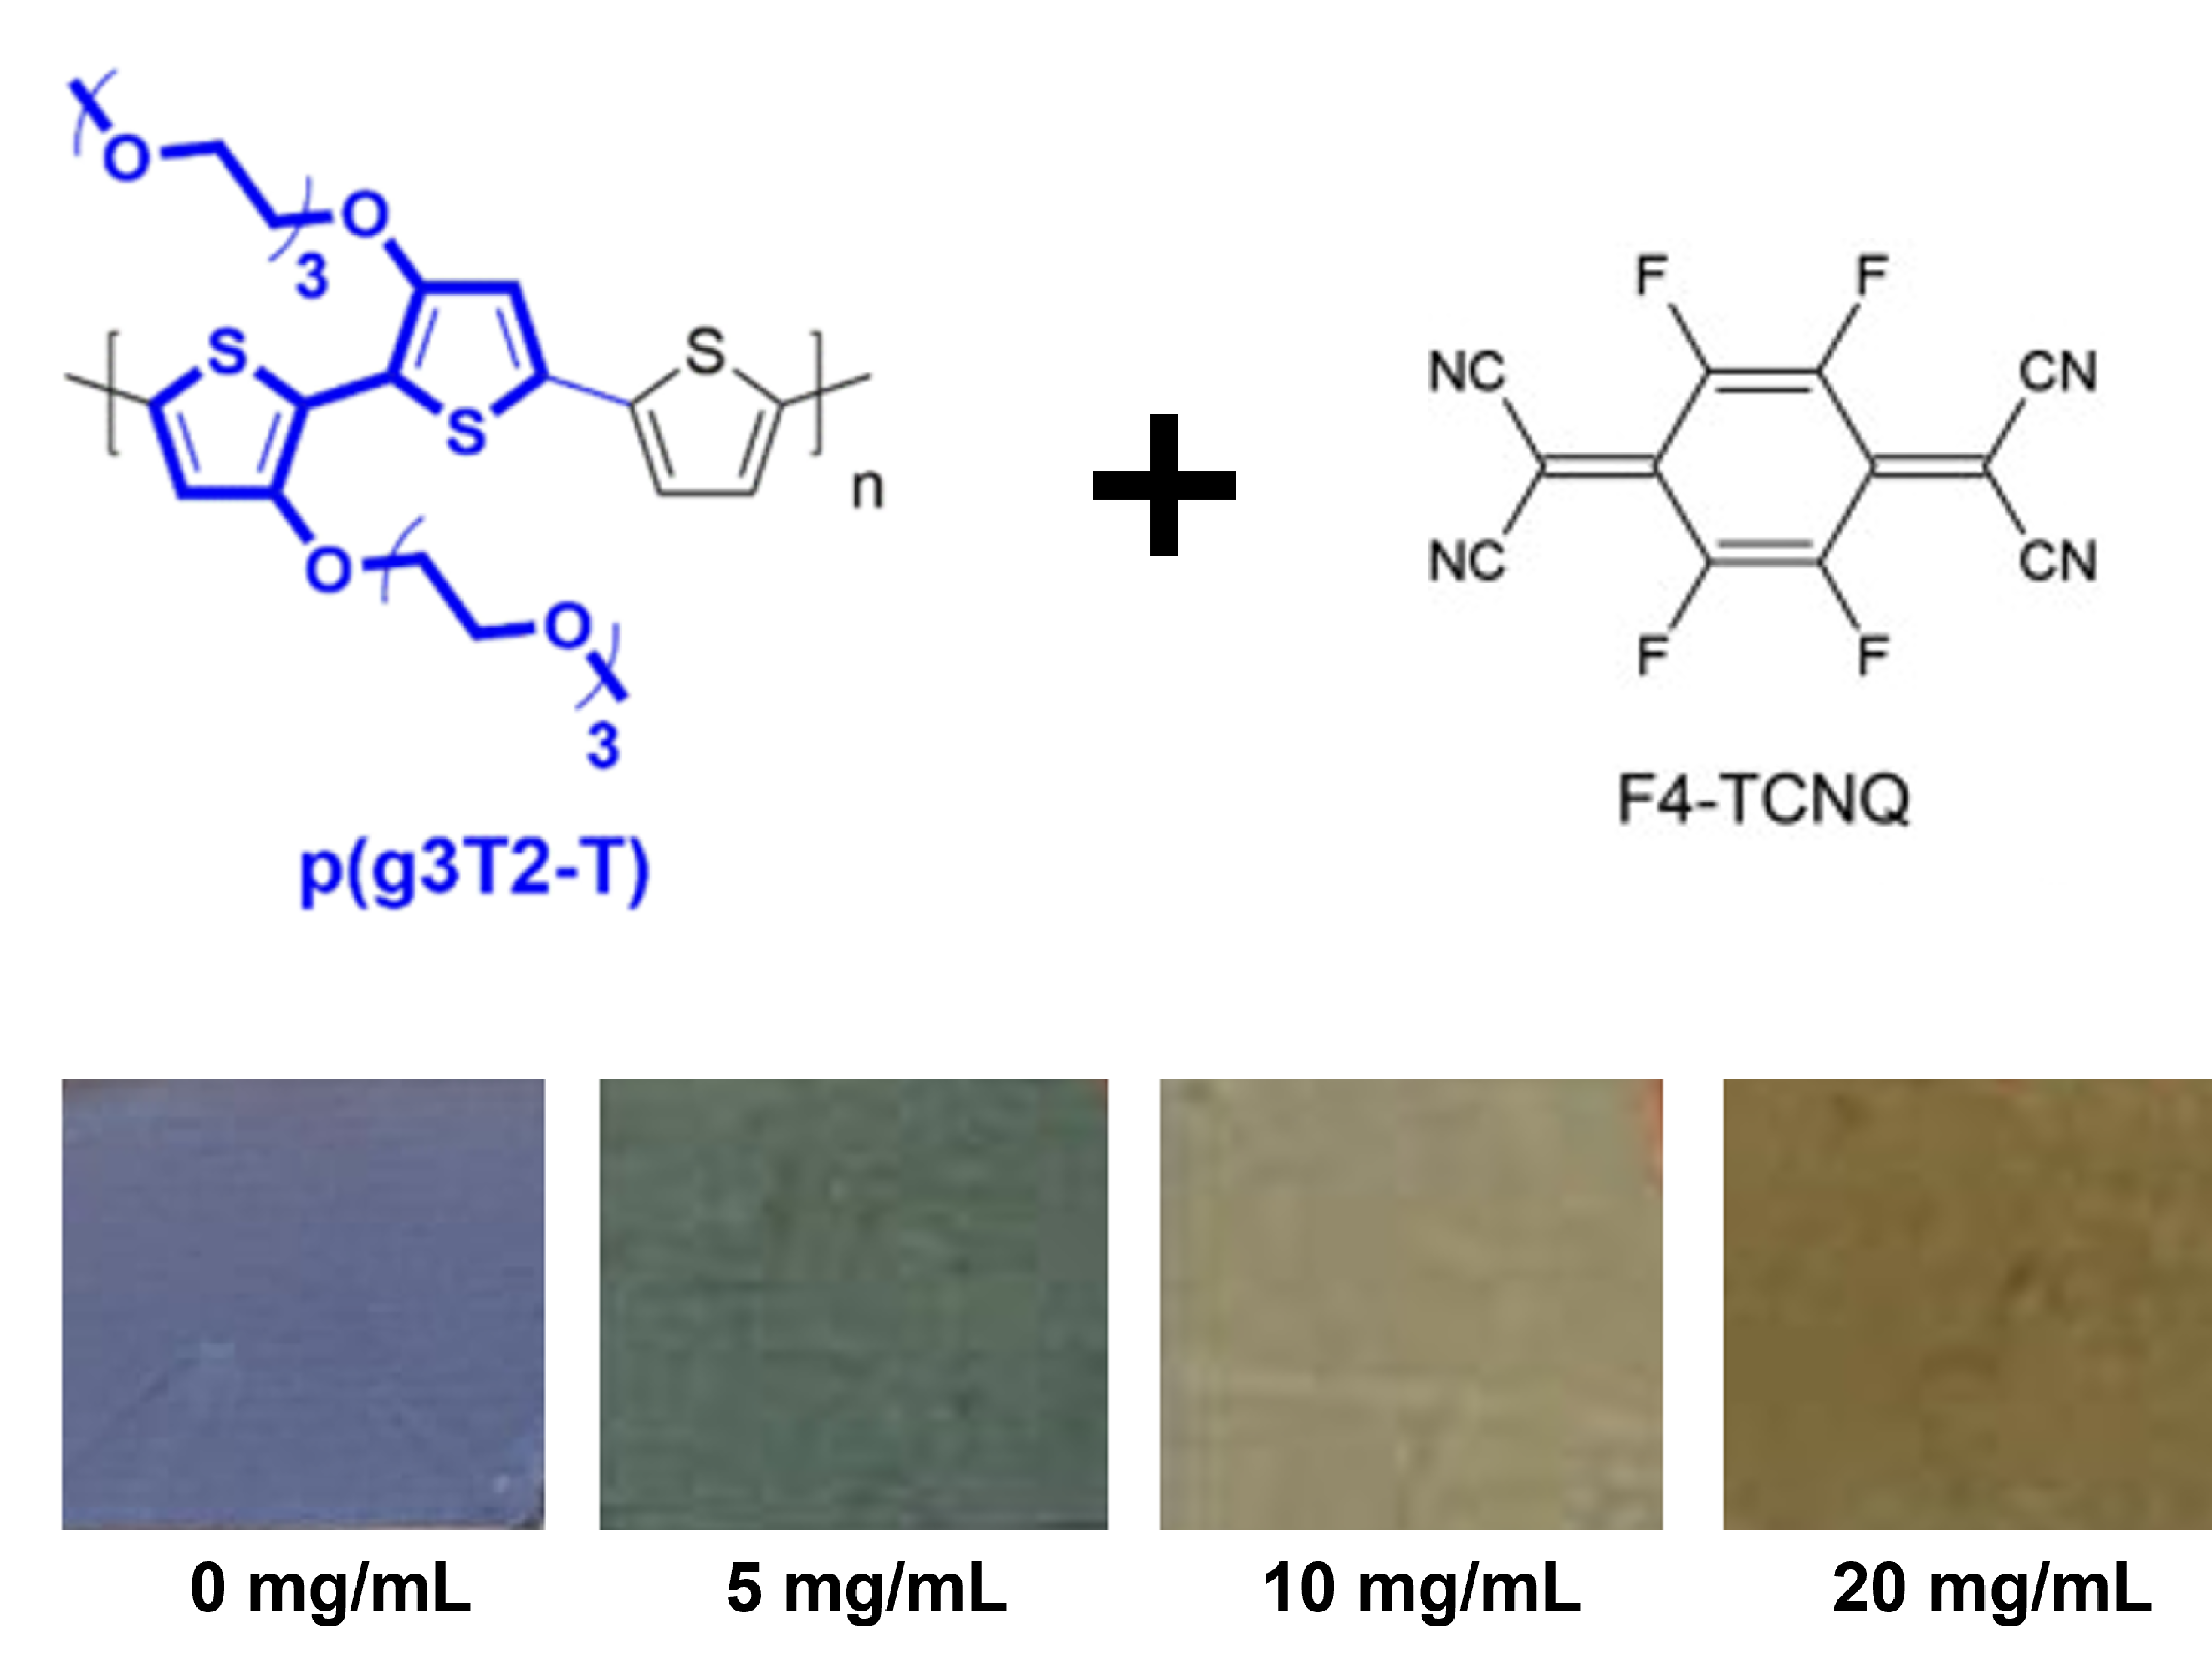
\includegraphics[width=8cm]{Images/pdf/doping_color.pdf}
  \caption[Color shift upon doping level increase]{(Top) Chemical structure of p(g3T2-T) and F$_{4}$TCNQ dopant. (Bottom) Color change upon increasing dopant concentration from 0 to 20 mg/mL.}
  \label{fig:color}
\end{figure}

\subsection{Absorbance and Dopants Diffusion}
The visible color hue shift can be described quasi-quantitatively by the absorbance spectra of the samples, as seen in Figure \ref{fig:abs}, where the undoped-p(g3T2-T) shows a prominent absorption peak at 588 nm (red), which diminishes with doping, characteristic from oxidation, and it is more intense with higher doping levels. New absorption peaks are seen at around 860 nm, this is due to generation of polarons that lead to new optical transitions, as explained in section... from the Background chapter. Tan et al. described the apparition of new absorption peaks within 300 to 600 nm, the higher energetic (lower wavelength) one is generated by unreacted neutral dopant species (TCNQ$^{0}$), while the second is due to the new dopant anions (TCNQ$^{-}$), the latter induce charges in our polymer \cite{tanTuningOrganicElectrochemical2022}. It is shown also, that after some days of storage, the initially dominant peak of unreacted neutral dopants is now lower in intensity than the anions peak, suggesting that the dopants were still diffusing through the polymer along the days. 

\begin{figure}[ht]
  \centering
  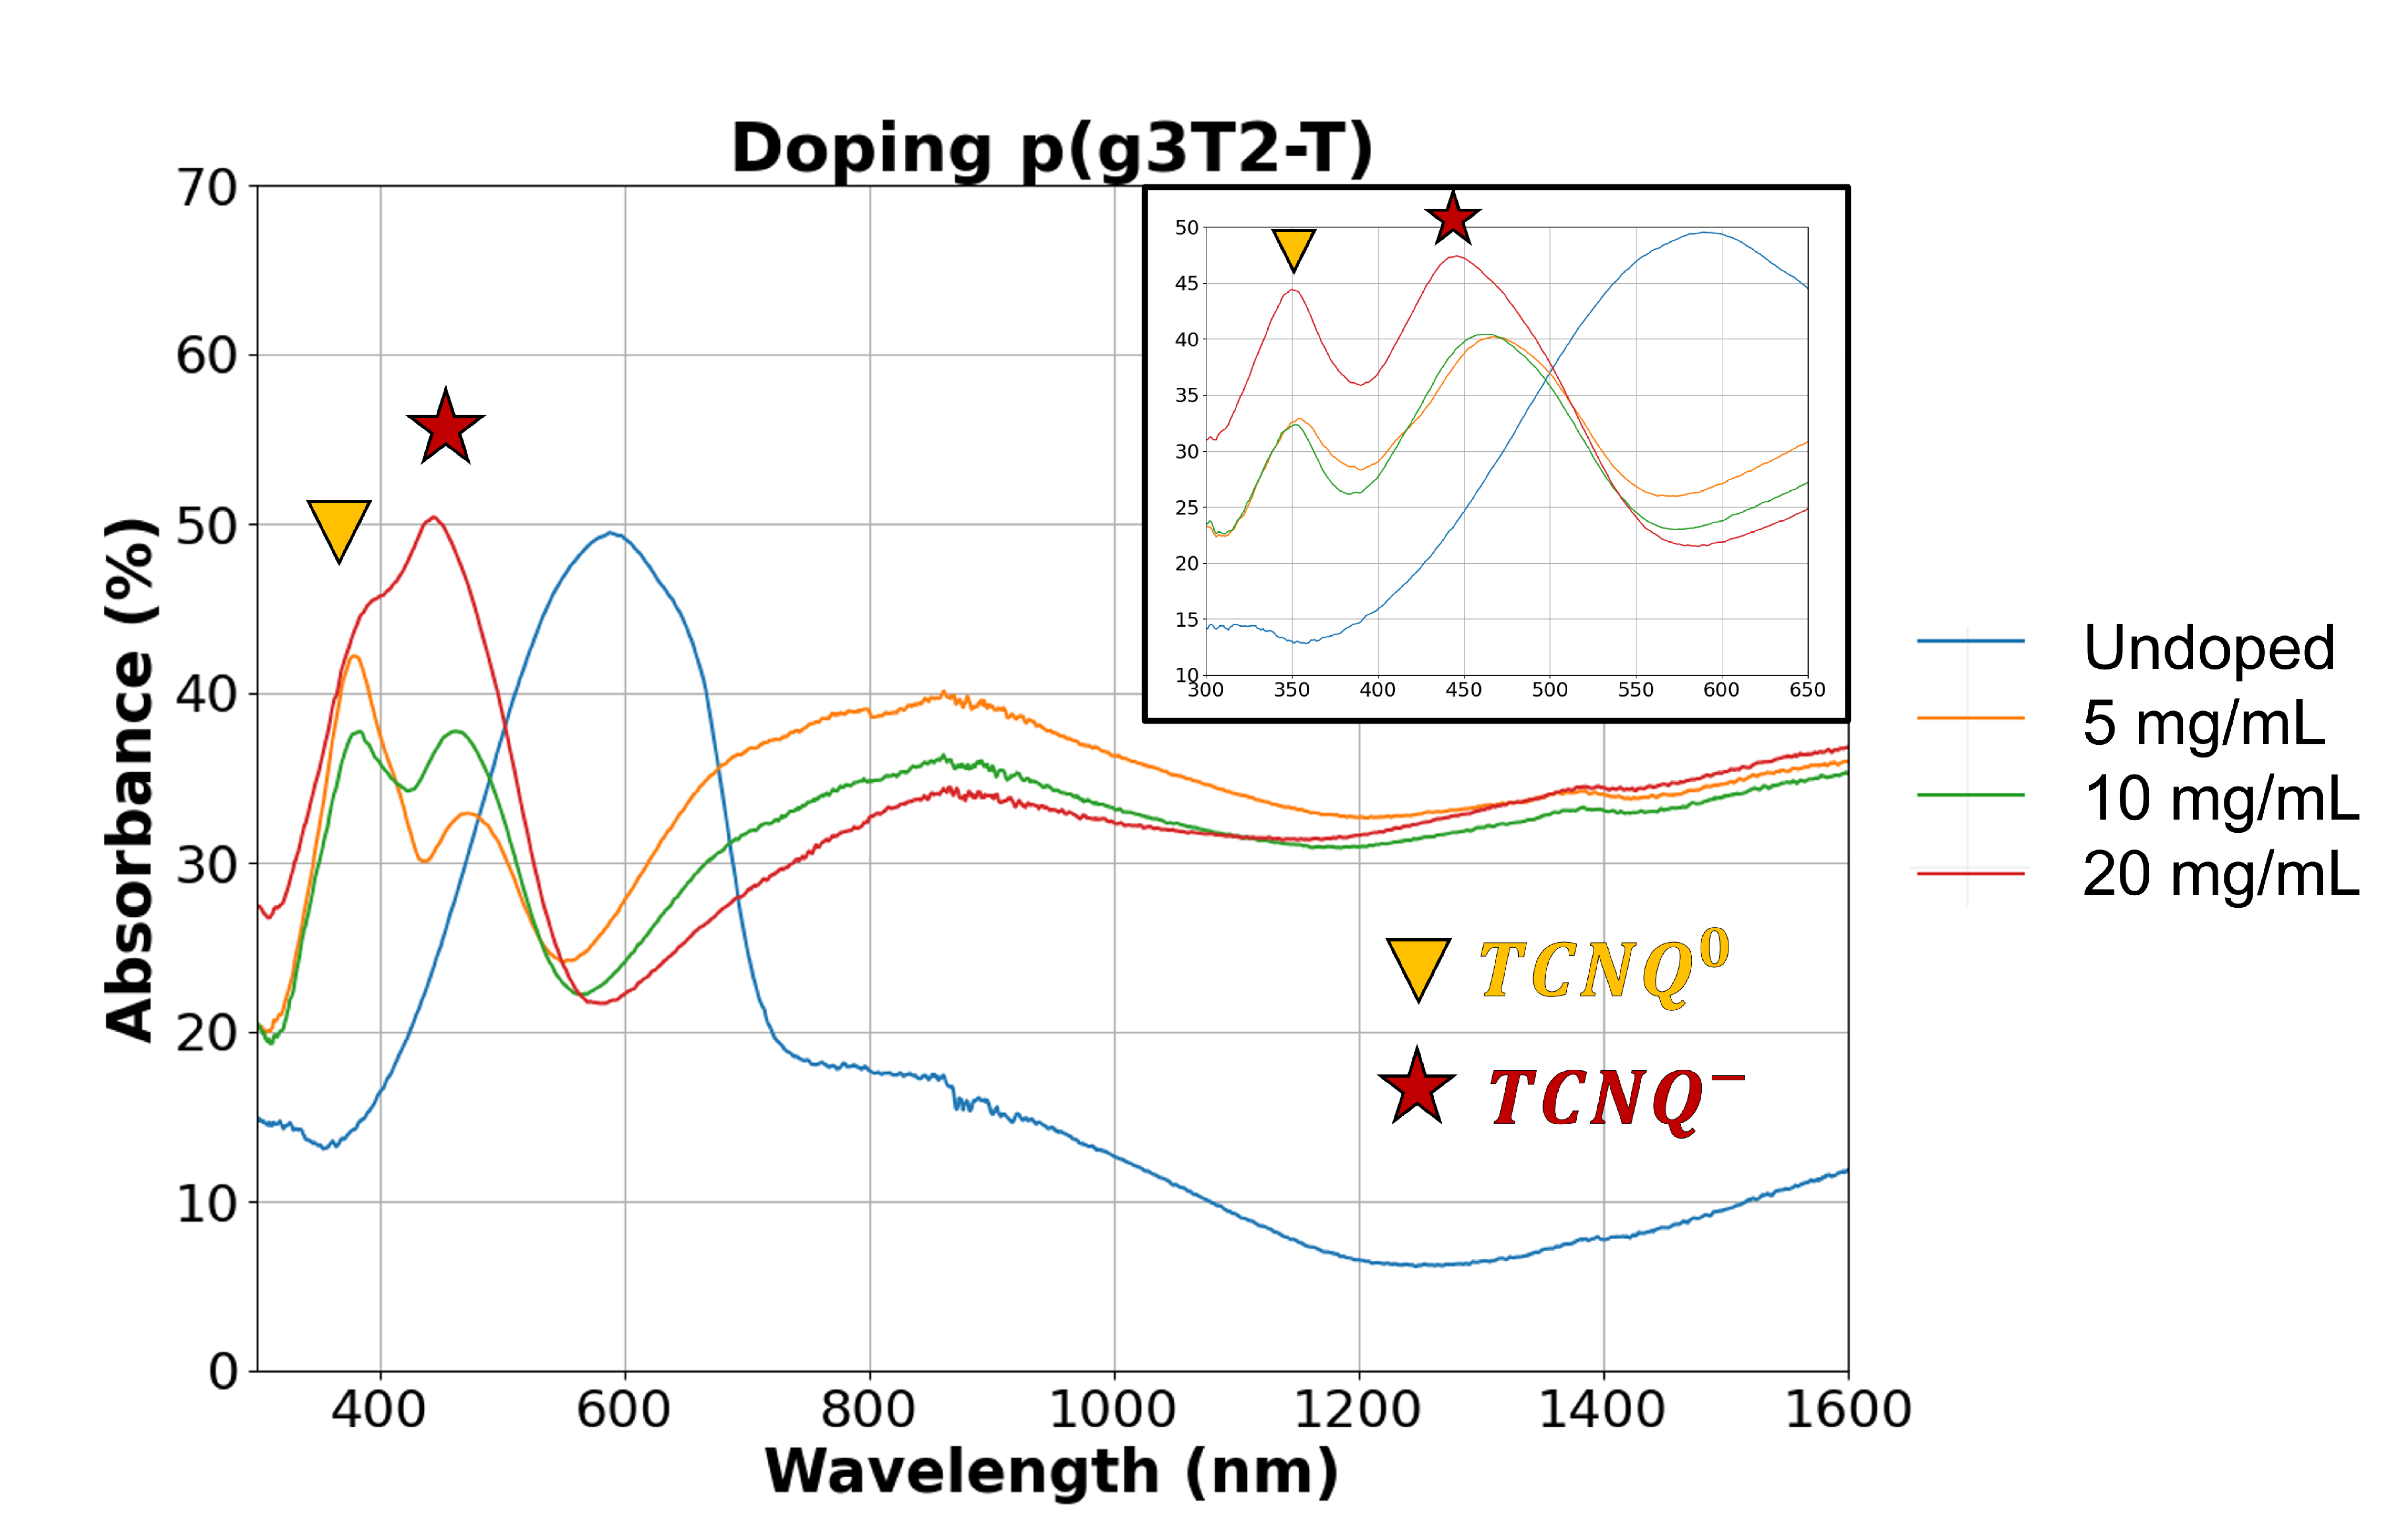
\includegraphics[width=\textwidth]{Images/pdf/abs+inlet.pdf}
  \caption[Absorbance spectra of different doping levels of p(g3T2-T)]{Spectra of undoped and doped-p(g3T2-T) at different doping levels, corresponding to samples on Figure \ref{fig:color}. Inlet represents absorbance after two weeks of storage in ambient conditions.}
  \label{fig:abs}
\end{figure}

Absorbance values are directly linked to the density of states of these new optical transitions \cite{bredasPolaronsBipolaronsSolitons1985}. From our spectra, the absorption value of the lowest doped-p(g3T2-T) (5 mg/mL) is higher (around 40\%), which may be counter-intuitive. However, as doping concentration increases, hence more electrons are taken out of the polymer chain, a bipolar is the energetically more favorable quasiparticle to generate. According to references \cite{tanTuningOrganicElectrochemical2022}\cite{enenglDopinginducedAbsorptionBands2016}, bipolaron formation is seen as a shift to lower energies in the broad absorbance the mid-IR region (wavenumber 1000-1600 cm$^{-1}$) so further analysis of hole bipolaron formation can be conducted with Fourier Transform InfraRed (FTIR) spectroscopy.
 
\subsection{Workfunction}

Although, the preparation of films for studying electron energy levels with UPS is ideally done under inert conditions to avoid any sort of contaminatio. The current fabrication process of OECTs inevitable exposes our films at ambient conditions. So measurements were taken following the deposition under ambient conditions. Yet, it is possible to distinguish an increase in the workfunction (shift of Fermi level) of the polymer. The Fermi level shift towards the HOMO level is higher at higher dopant levels, as represented in Figure \ref{fig:ups}, characteristic of p-type doping. Some possible additional contamination did not allow to measure sample with 20 mg/mL of dopant, but tendency is evident.

\begin{table}[ht]
\centering
\caption{Workfunction calculation from UPS measurements.}
\begin{tabular}{l|c|c|c}
& Undoped & 5 mg/mL & 10 mg/mL \\\hline
E$_{HBEC}$ [eV] & 17.35 & 16.47 & 16.36\\
E$_{HOMO}$ (vs E$_{F}$) & 4.28 & 3.27 & 3.24\\
WF [eV] & 3.87 & 4.28 & 4.86\\\hline
\end{tabular}
\label{tab:ups}
\end{table}

It is important to consider that UPS is a surface sensitive measurement, the penetration depth of the ultraviolet range electrons are around 2 nm, which is significantly lower than our polymer thickness (around 70 nm). So this technique limits our understanding of the dopants diffusion through the whole volume of the polymer. Although, we had some insights of this topic from the previous section, further analysis could be done with X-Ray Photoelectron Spectroscopy that has a higher penetration depth (around 5 nm), again also limited. %but along with depth profiling mode 

\begin{figure}[ht]
  \centering
  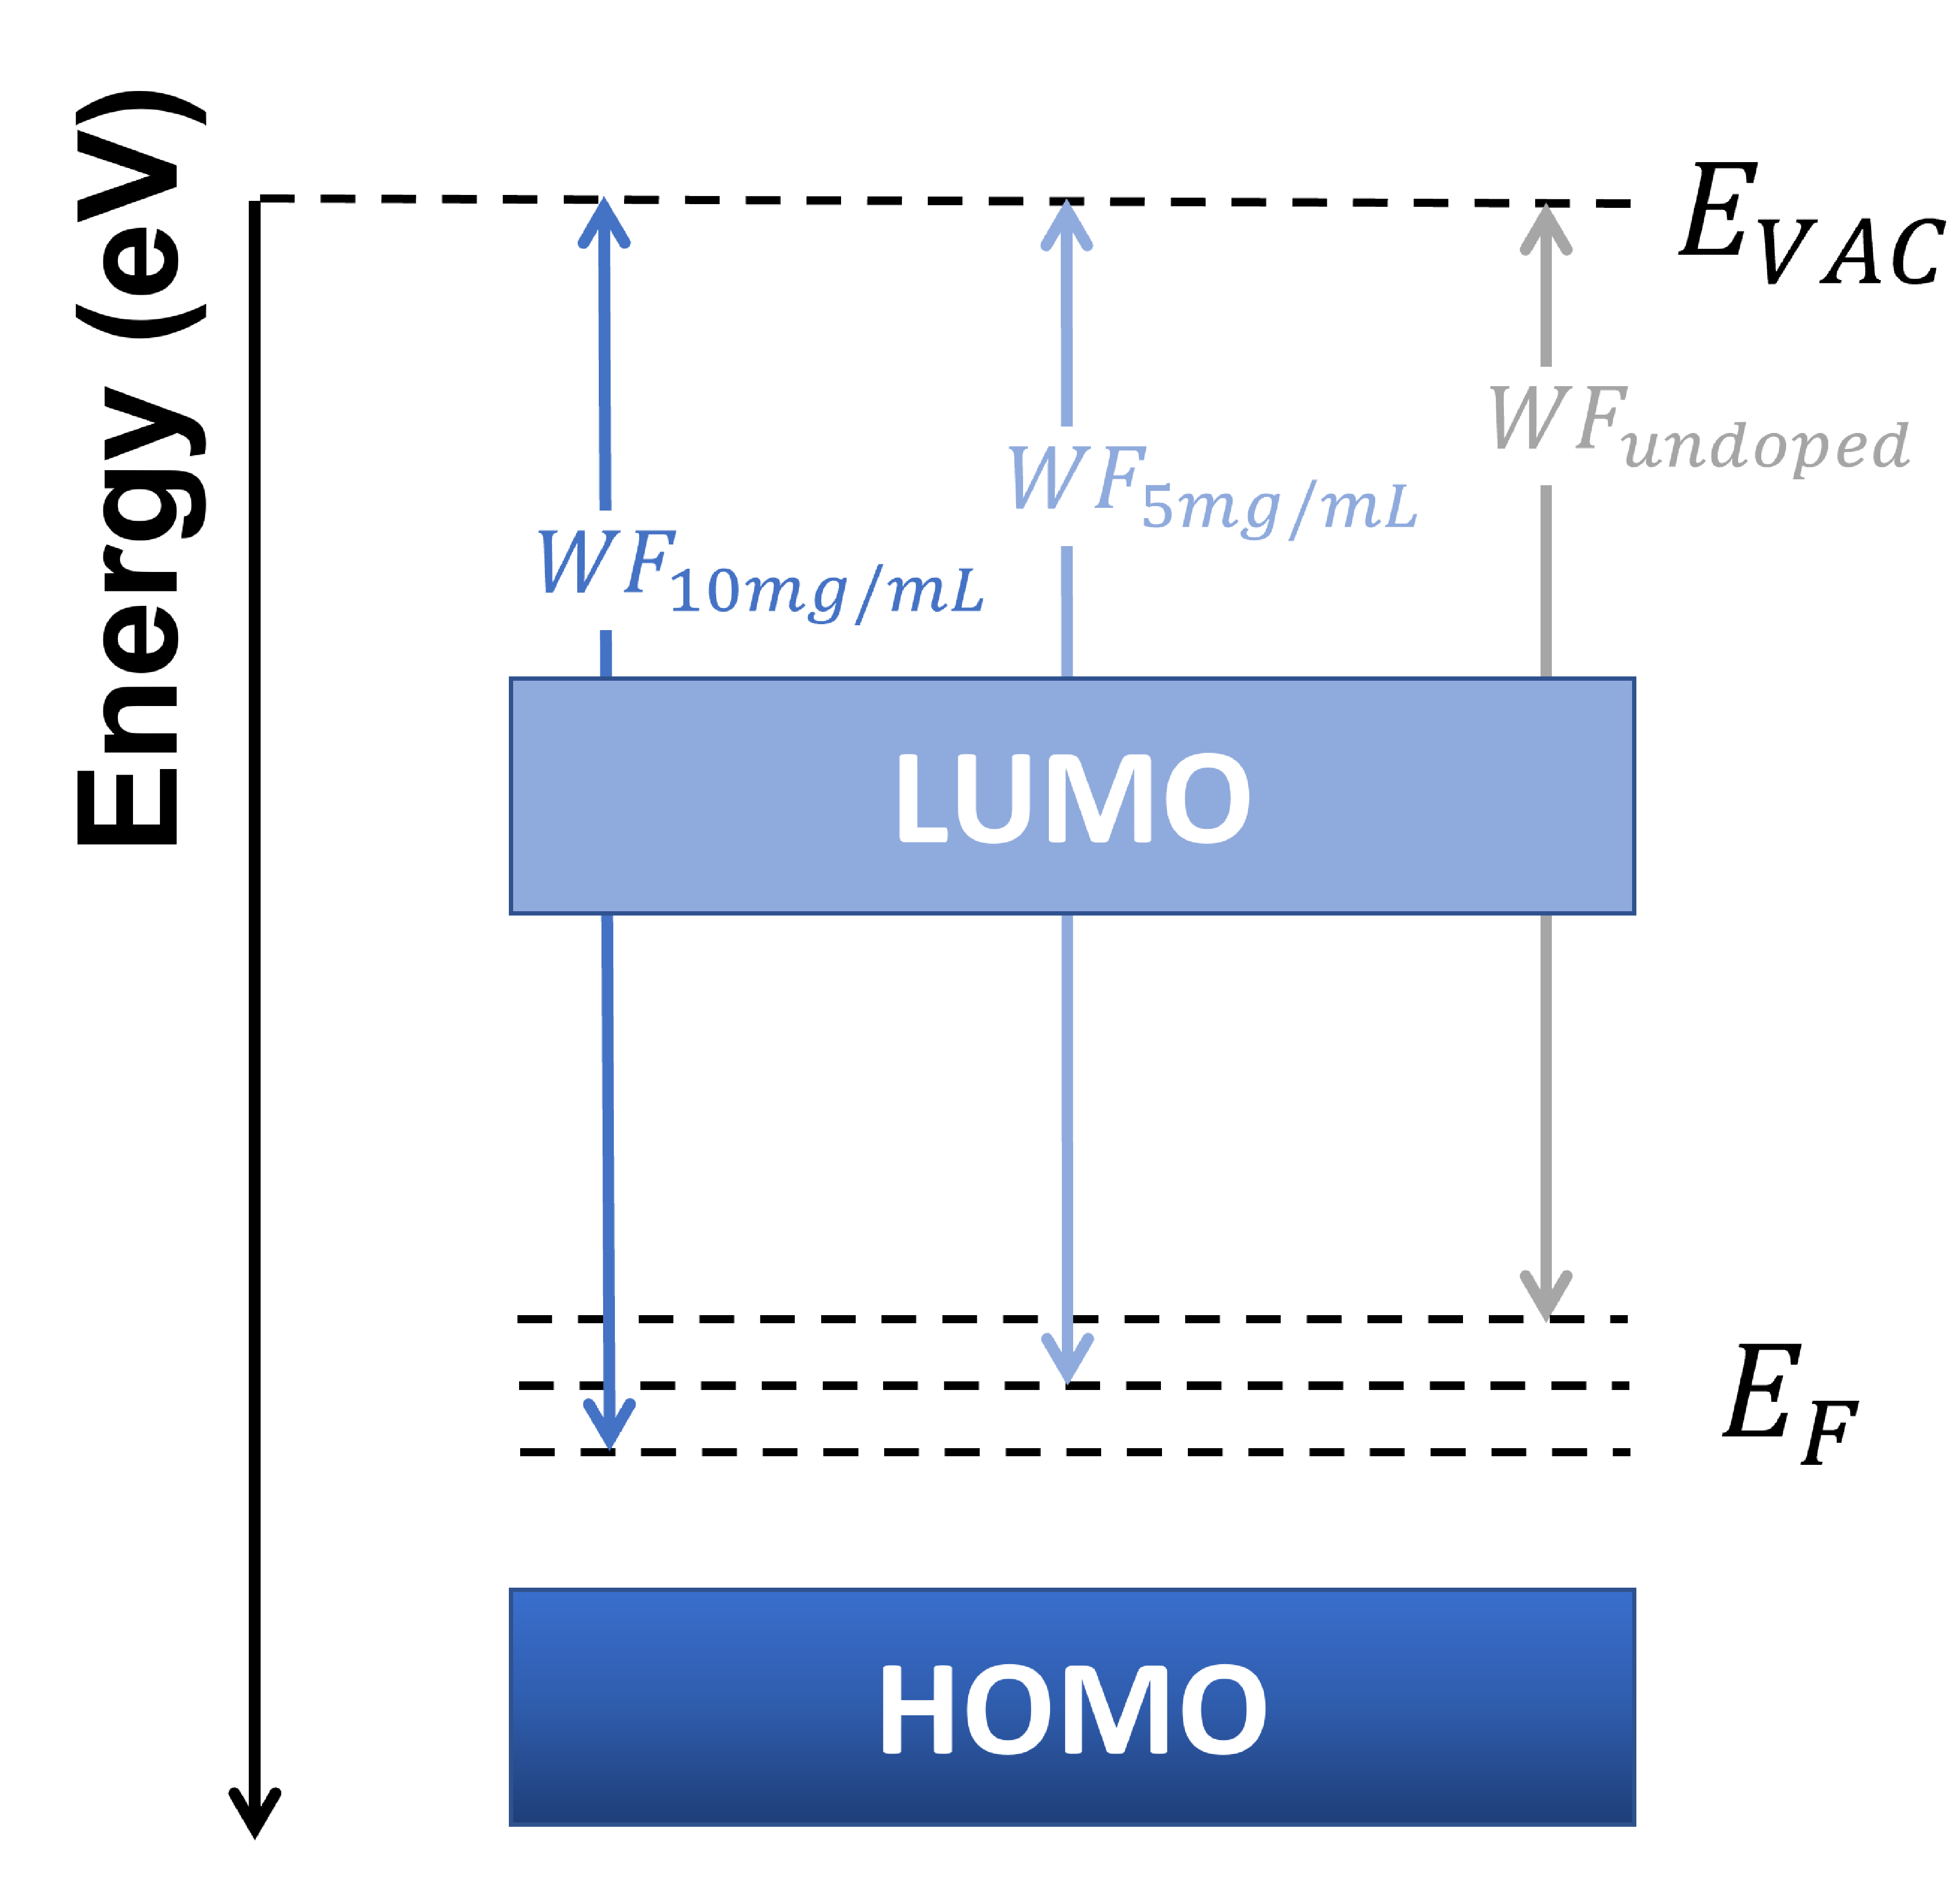
\includegraphics[width=8cm]{Images/pdf/WF.pdf}
  \caption[Representation of the Fermi level shift upon doping]{Representation of the Fermi level shift for doped-p(g3T2-t)}
  \label{fig:ups}
\end{figure}

\subsection{Thickness, Sheet Resistance and Resistivity}

Sheet resistance and resistivity shown in Table \ref{tab:res} were calculated using equations \ref{eq:rs} and \ref{eq:resist}, respectively, described in previous chapter. The film thickness was obtained with profilometer measurements, yielding to approximate 70 nm.

\begin{table}[ht]
\centering
\caption{Sheet resistance and resistivity calculations for undoped and doped films of p(g3T2-T)}
\begin{tabular}{l|c|c|c|c}
& Undoped & 5 mg/mL & 10 mg/mL & 20 mg/mL \\\hline
Sheet resistance ($\Omega$/sq) & 6.3M & 104.6k & 70.7k & 49.4k\\
Resistivity ($\Omega$cm) & 44.1 & 0.73 & 0.49 & 0.35\\\hline
\end{tabular}
\label{tab:res}
\end{table}

Upon doping there is a major decrease in both parameters, which is not as significant when adding more dopants, as seen in Figure \ref{fig:rho}. However, if comparing the decrease among doped samples, we could perceived a linear dependency upon increasing the dopant concentration. 

\begin{figure}[ht]
  \centering
  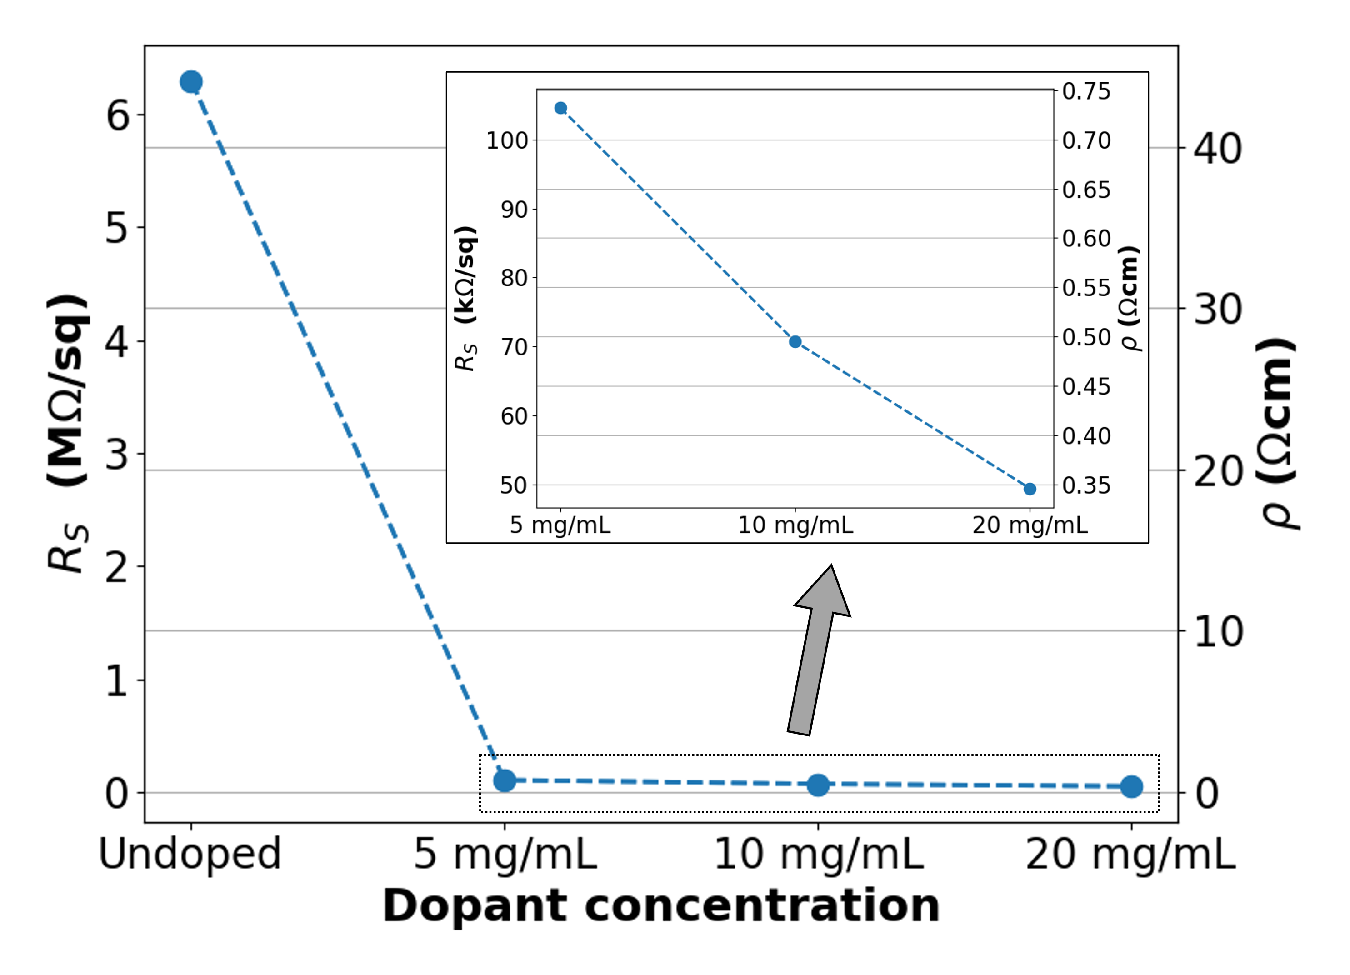
\includegraphics[width=10cm]{Images/pdf/resist+inlet.pdf}
  \caption[Sheet resistance and resistivity drop upon doping]{Sheet resistance and resistivity drop upon doping of p(g3T2-T). Inlet represents the quasi-linear drop of parameters as between doped samples.}
  \label{fig:rho}
\end{figure}

%\subsection{Roughness}

\section{Fabrication of Organic Electrochemical Transistors}

%Prior biasing gate, which is due to passive (ion) diffusion?

\subsection{Influence of Doping OECT Channel}
The fabrication process used a mask that include a microstructure gate, available for studying OECTs with channel and gate made of the same OMIEC material (commonly PEDOT:PSS). The result of the patterning process is shown in Figure \ref{fig:channel}. However, in this part, we are going to test only the OMIEC channel (p(g3T2-T) at different doping levels) with a non-polarizable gate such as Ag/AgCl pellet, using dropcasted solid-state electrolyte precursor to couple both channel and gate. Unfortunately, the sample that used solution with 20 mg/mL dopant concentration showed homogeneity issues that still allow photolithography but could not represent a fair comparison with the other devices, so it will be disregarded in this analysis.

\begin{figure}[ht]
  \centering
  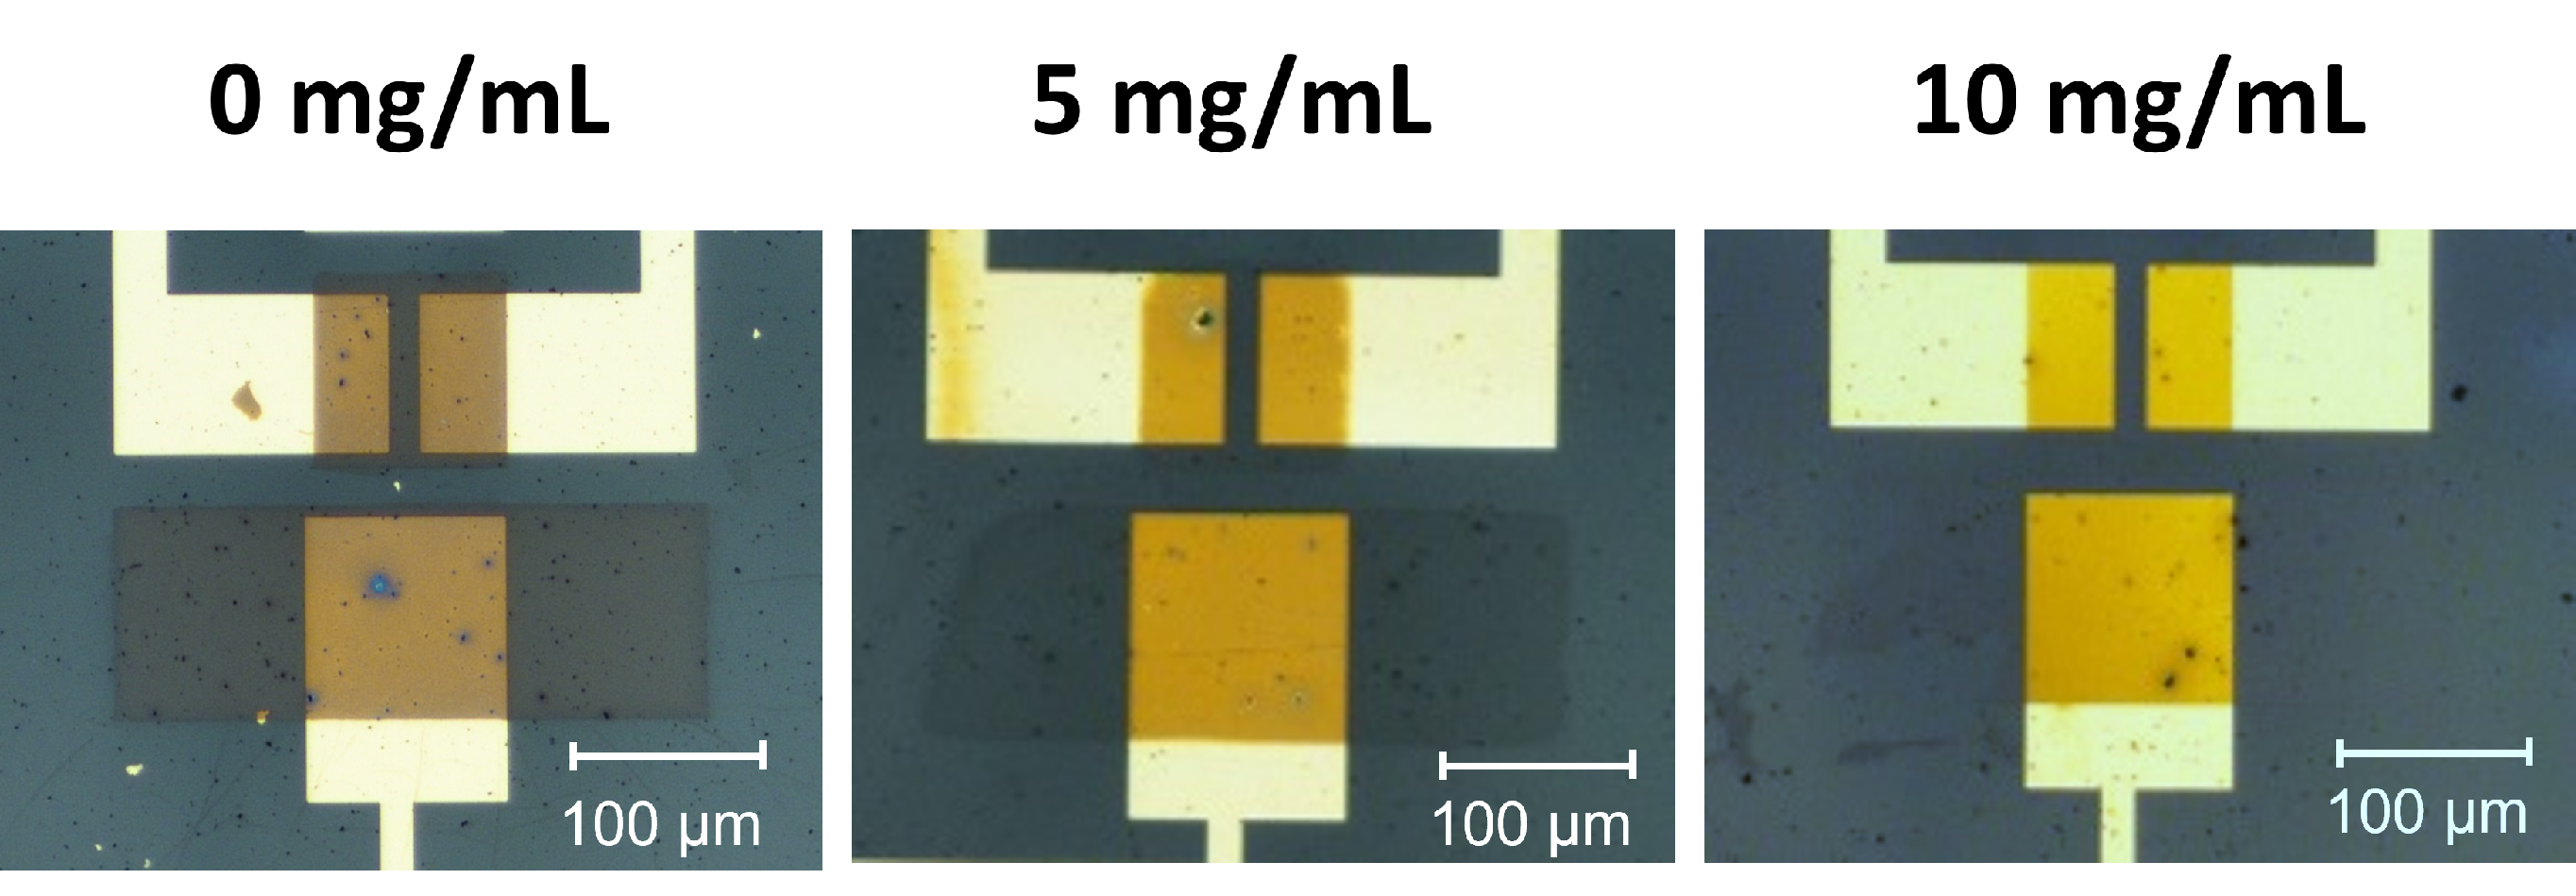
\includegraphics[width=10cm]{Images/pdf/BigGateDevices.pdf}
  \caption[Micrographs of a patterned channel and gate p(g3T2-T) at different doping levels]{Micrographs of patterned channel and gate with undoped, 5 mg/mL and 10 mg/mL doped p(g3T2-T) following procedures explained in Section \label{subsec:photo}.}
  \label{fig:channel}
\end{figure}

%U4 loop 2 as undoped pattern
%U2 loop 3 for doped 5
%U4 loop 3 for doped 10

\begin{figure}[ht]
    \centering
    \subfloat[]{{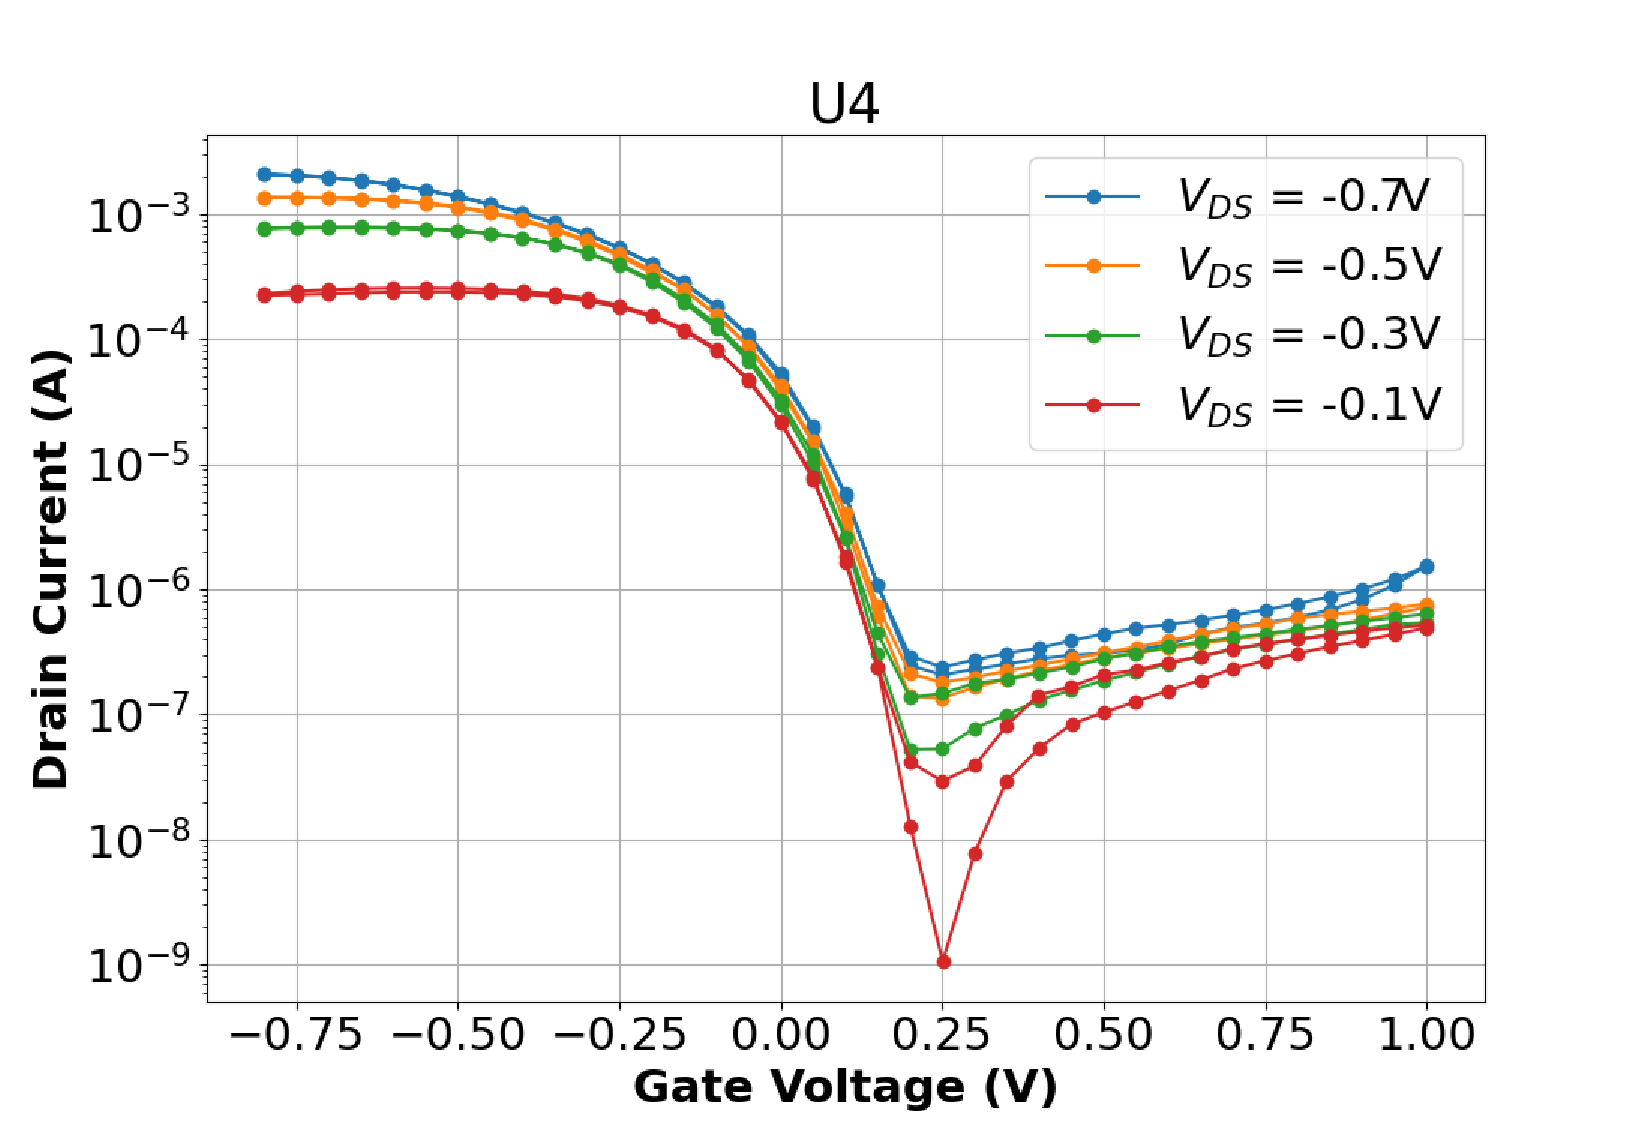
\includegraphics[height=5.5cm]{Images/pdf/transfer_undoped.pdf} }}
    \subfloat[]{{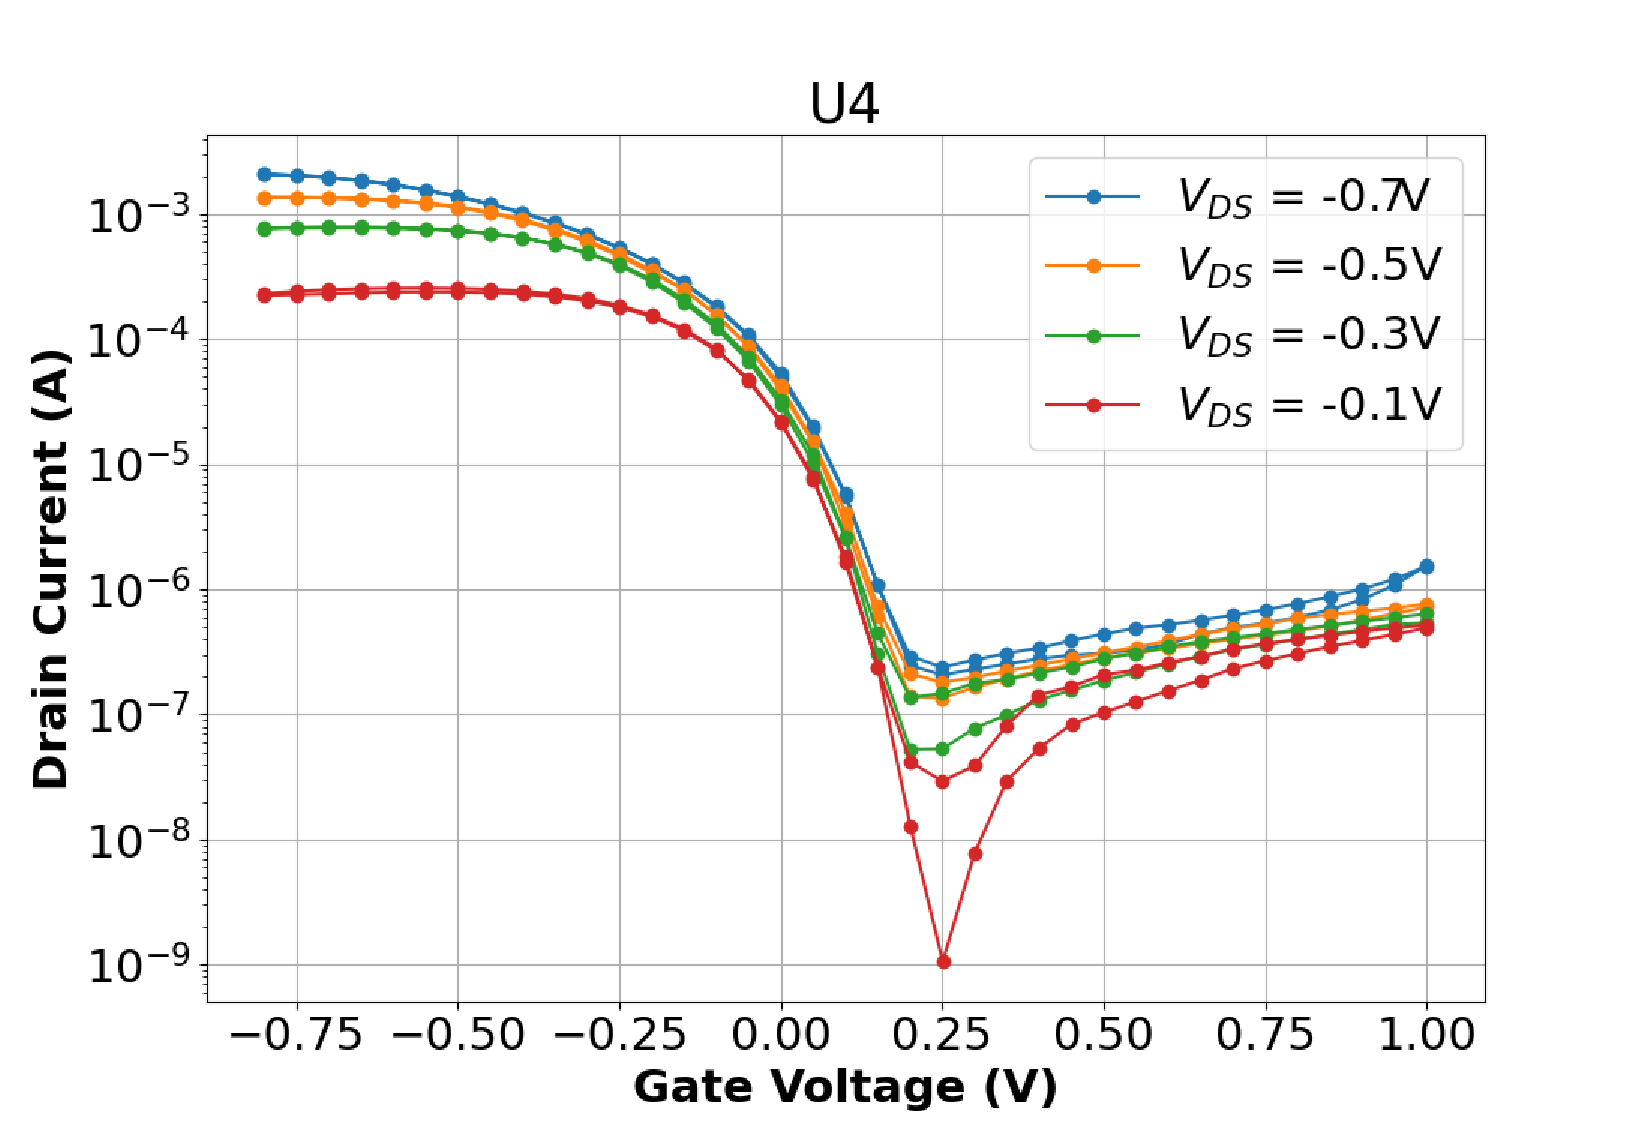
\includegraphics[height=5.5cm]{Images/pdf/transfer_undoped.pdf} }}
    \qquad
    \subfloat[]{{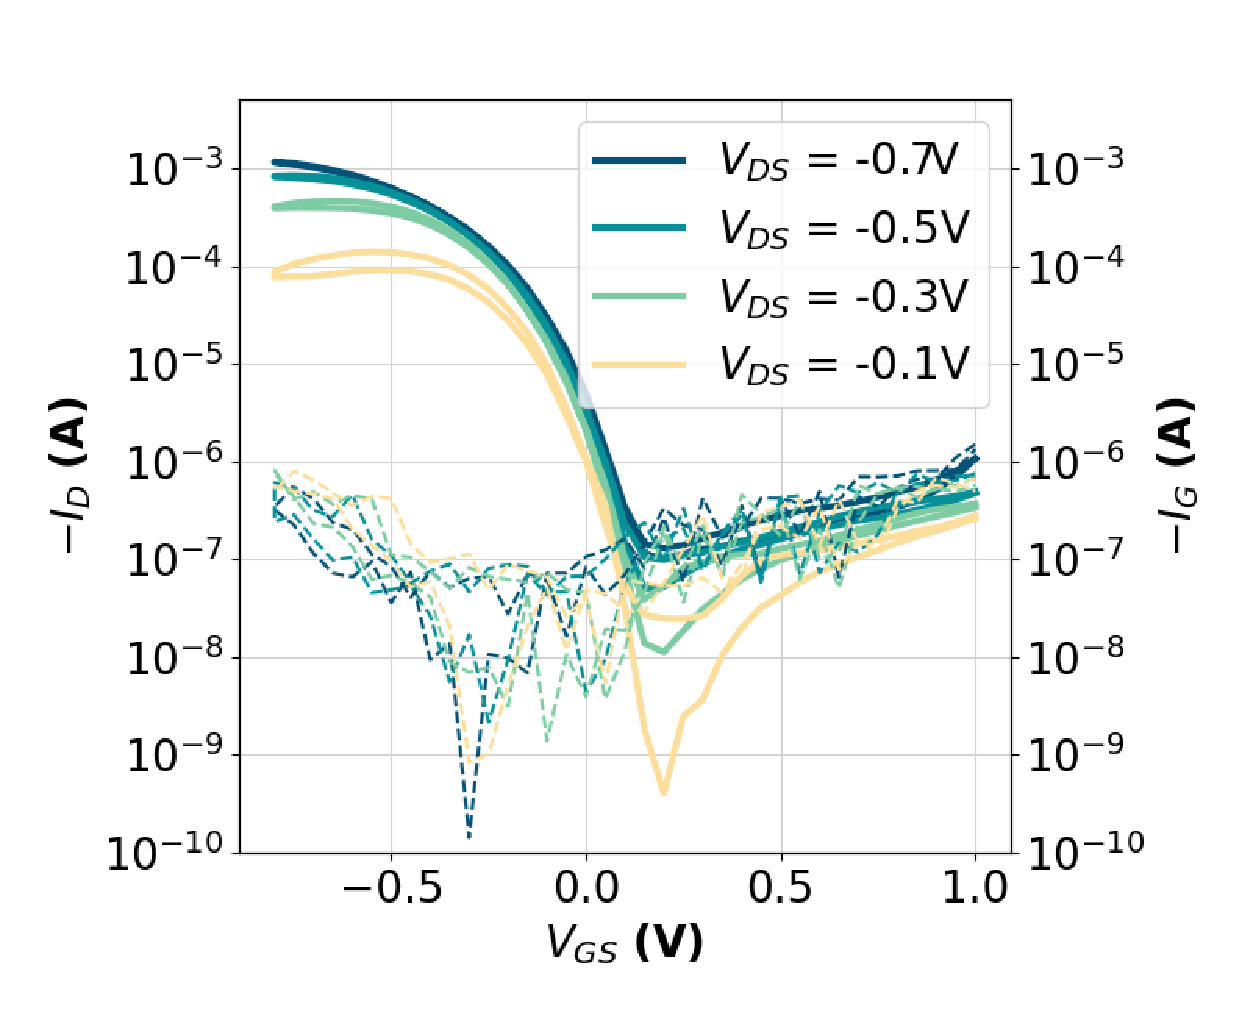
\includegraphics[height=5.5cm]{Images/pdf/transfer_doped5.pdf} }}
    \subfloat[]{{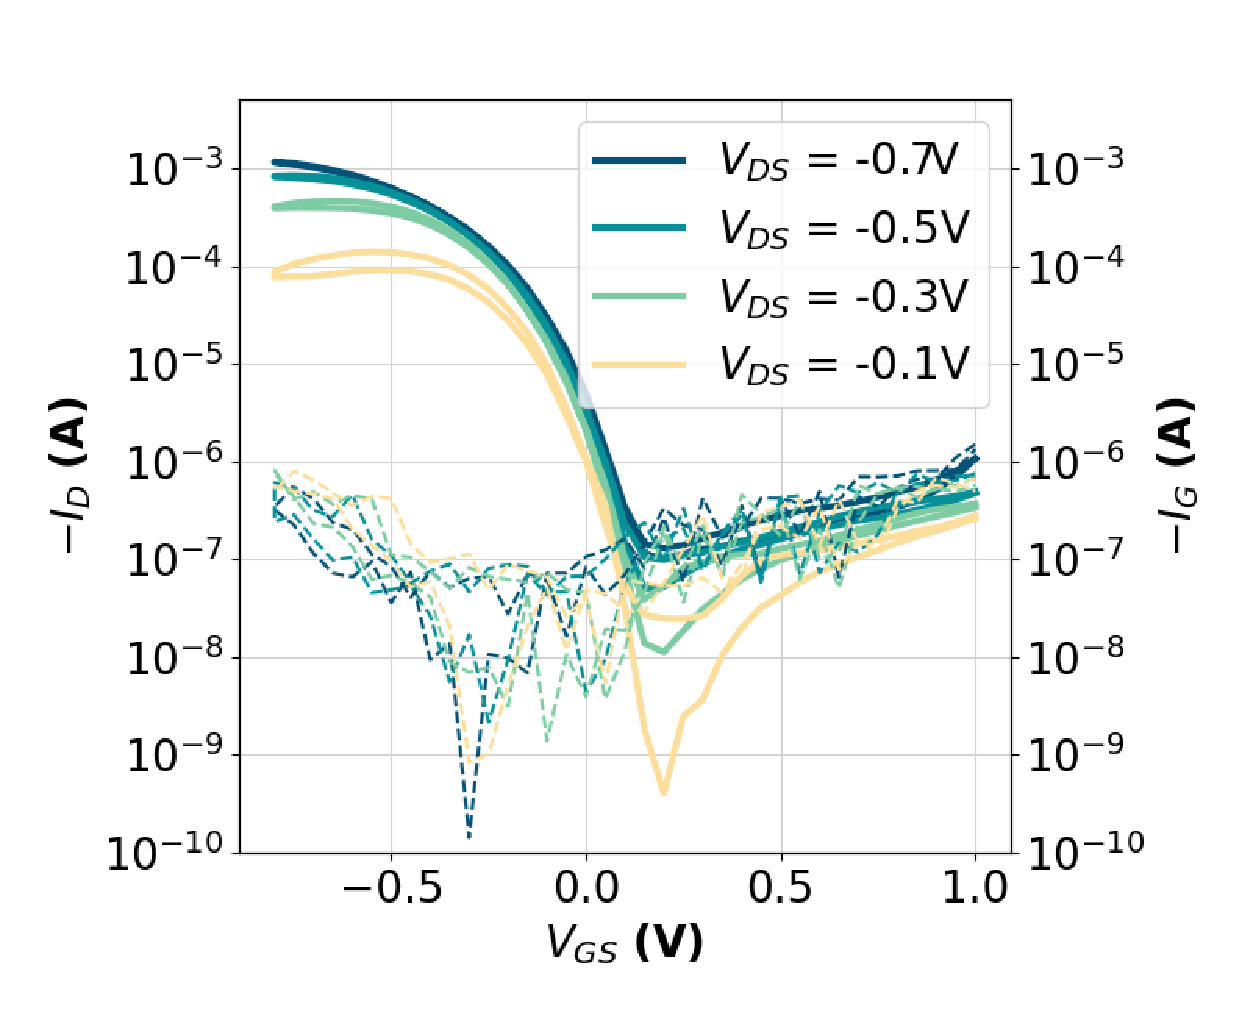
\includegraphics[height=5.5cm]{Images/pdf/transfer_doped5.pdf} }}
    \qquad
    \subfloat[]{{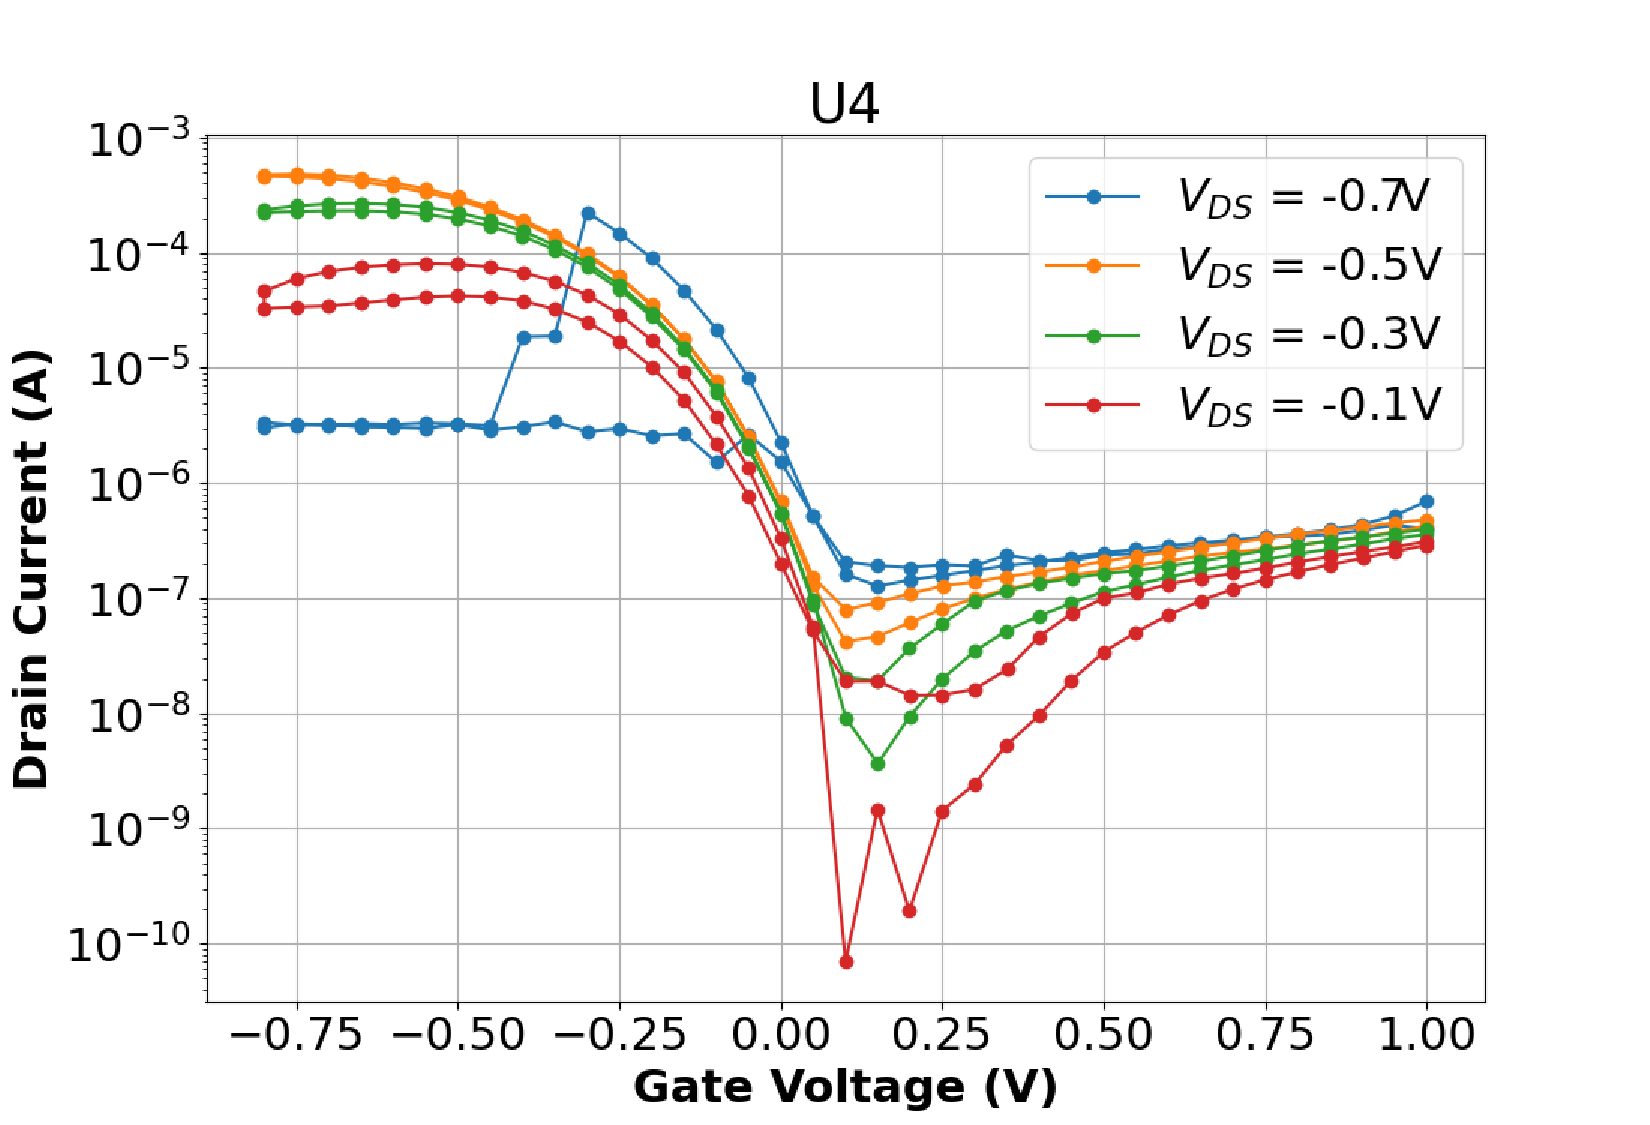
\includegraphics[height=5.5cm]{Images/pdf/transfer_doped10.pdf} }}
    \subfloat[]{{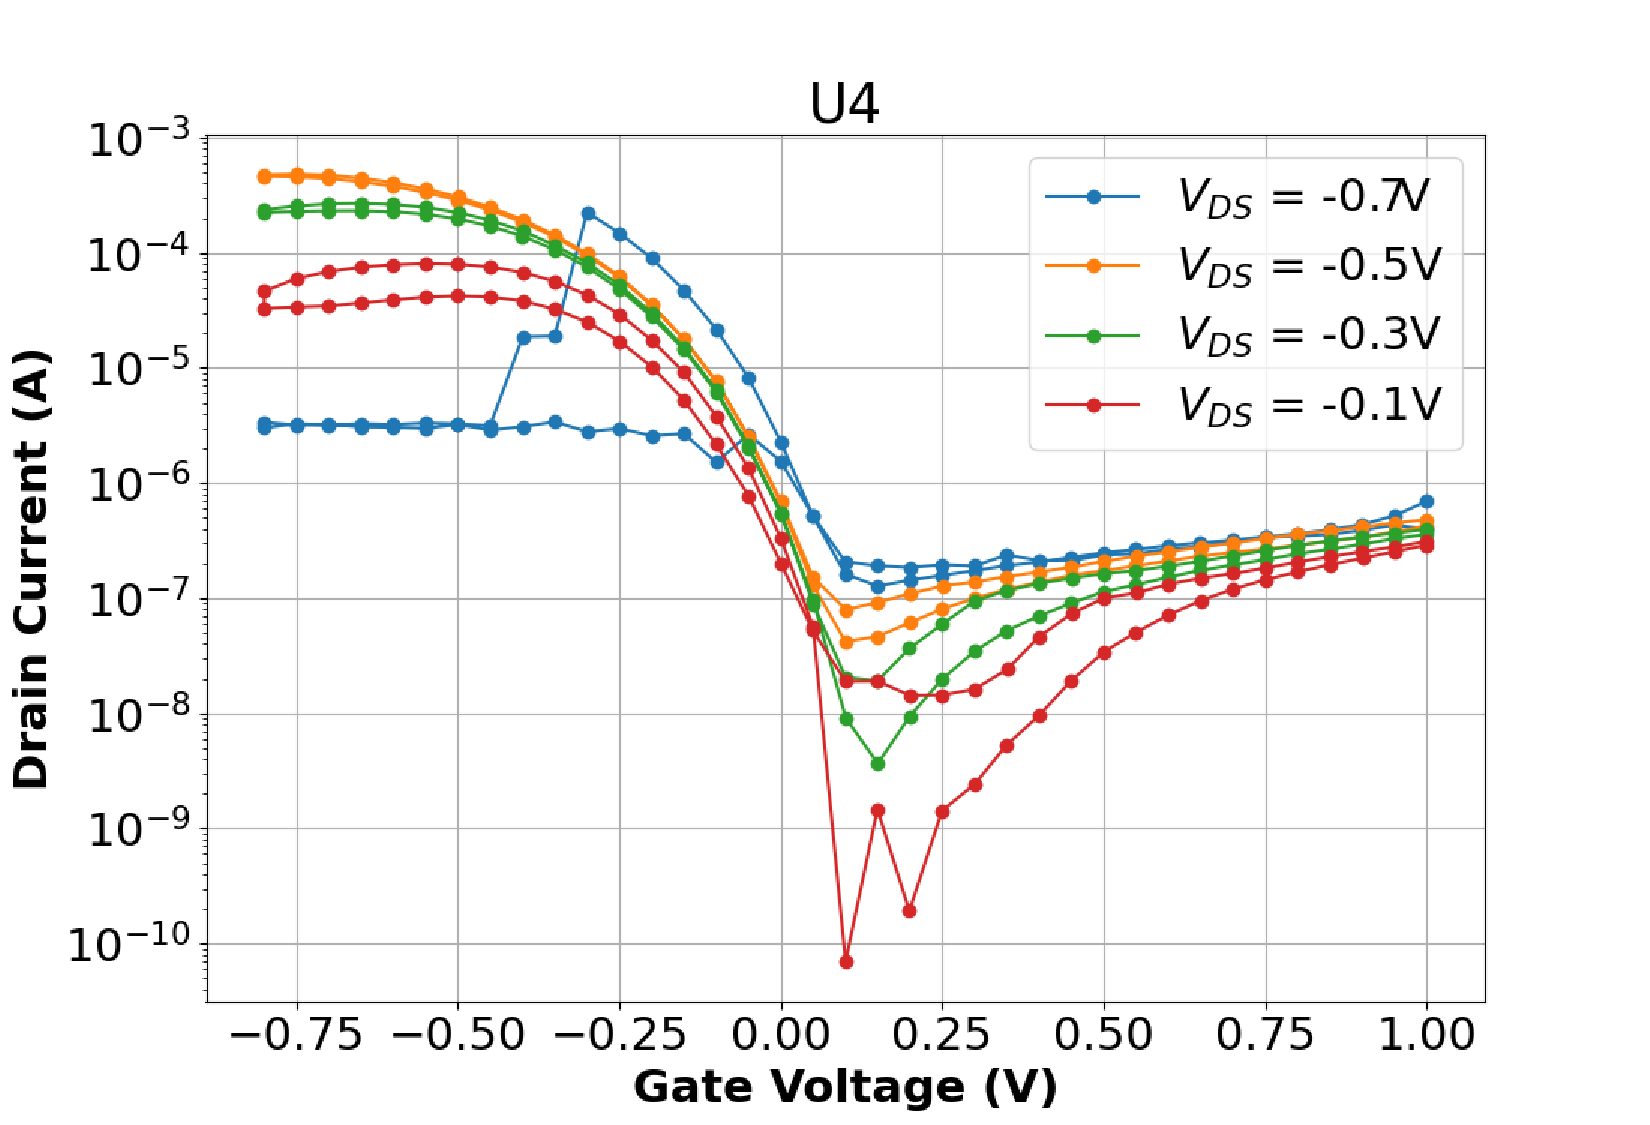
\includegraphics[height=5.5cm]{Images/pdf/transfer_doped10.pdf} }}
    \caption{Transfer characteristics and transconductance at different V$_{DS}$. a), c) and e) correspond to the exponential behavior of undoped, 5 mg/mL and 10 mg/mL doped, respectively.}
    \label{fig:transfercurves}
\end{figure}

\begin{table}[ht]
\centering
\caption{Maximum transconductance and $\mu$C* product calculation}
\begin{tabular}{l|c|c|c}
& Undoped & 5 mg/mL & 10 mg/mL \\\hline
g$_{m,max}$ [mS] & 17.35 & 16.47 & 16.36\\
$\mu$C* [Fcm$^{-1}$V$^{-1}$s$^{-1}$] & 4.28 & 3.27 & 3.24\\\hline
\end{tabular}
\label{tab:fom}
\end{table}


\subsection{Stability on Air of p(g3T2-T)}

\subsection{Reverse Oxidation of Undoped-p(g3T2-T}

\subsubsection{By Electrochemical Dedoping}

\subsubsection{By Heating}


\subsection{Solid-OECTs using Undoped p(g3T2-T)}


%The Ag/AgCl gate electrode’s work function is reasonably constant, the work function of an OMIEC gate electrode however may vary depending on its processing history and redox reactions with other species present in the electrolyte (e.g. molecular oxygen).28 Applying VGS only determines the potential difference between the gate and channel but does not control the potentials of either electrode (hence the position of the Fermi level) with respect to a reference. This leads to many challenges in operating an OECT with OMIEC gate electrodes.


\subsubsection{Dropcasted Solid-State Electrolyte}

\subsubsection{OECT with Dropcast Solid-State Electrolyte}

\subsubsection{OECT with Photopatternable Solid-State Electrolyte}

\subsubsection{OECT with Inkjet-Printed Solid-State Electrolyte}


\subsection{Solid-OECTs using Doped-p(g3T2-T)}

\begin{figure}
  \centering
  \includegraphics[width=10cm]{Images/pdf/dopingprocess.pdf}
  \caption[Energy diagram of p(g3T2-T) and dopants F$_{6}$TCNNQ and F$_{4}$TCNNQ]{Energy diagram of p(g3T2-T) with a) F$_{6}$TCNNQ and b) F$_{4}$TCNNQ. Ionization potential of p(g3T2-T) extracted from reference \cite{tanTuningOrganicElectrochemical2022} and electron affinities of the neutral species (EA$^{0}$) and of the anion (EA$^{-}$) of the dopants are extracted from cyclic voltammetry measurements in reference \cite{kieferDoubleDopingConjugated2019}.}
  \label{fig:doping}
\end{figure}

%Achieving effective charge transfer between the analyte and OMIEC requires appropriate alignment of the electrochemical potential of electrons on the OMIEC electrode and the redox specie. Failure to do so may result in the subsequent transfer of charges to other redox-active sinks in the environment, leading to undesirable side reactions and products that may interfere with the OMIEC’s operation. Electrons flow from a region of higher to lower electrochemical potential. Hence, achieving electron transfer from redox-active species to the OMIEC requires the latter to have a deep LUMO (high electron affinity) \cite{tanMixedIonicElectronic2022} %paper

%\section{Conclusion}
%\lipsum[86-88]

%%% Local Variables: 
%%% mode: latex
%%% TeX-master: "thesis"
%%% End: 

%\chapter{Results and Discussion}
\label{cha:3_empty}

\section{Doping Characterization}

\subsection{Absorbance and Dopants Diffusion}

\subsection{Workfunction}


\subsection{Thickness, Sheet Resistance and Resistivity}

%\subsection{Roughness}

\section{Fabrication of Organic Electrochemical Transistors}

%Prior biasing gate, which is due to passive (ion) diffusion?

\subsection{Influence of Doping OECT Channel}


\subsection{Stability on Air of p(g3T2-T)}

\subsection{Reverse Oxidation of Undoped-p(g3T2-T)}

\subsubsection{By electrochemical dedoping}

\subsubsection{By heating}


\subsection{Solid-OECTs using Undoped p(g3T2-T)}


%The Ag/AgCl gate electrode’s work function is reasonably constant, the work function of an OMIEC gate electrode however may vary depending on its processing history and redox reactions with other species present in the electrolyte (e.g. molecular oxygen).28 Applying VGS only determines the potential difference between the gate and channel but does not control the potentials of either electrode (hence the position of the Fermi level) with respect to a reference. This leads to many challenges in operating an OECT with OMIEC gate electrodes.


\subsubsection{Dropcasted Solid-State Electrolyte}

\subsubsection{OECT with Dropcast Solid-State Electrolyte}

\subsubsection{OECT with Photopatternable Solid-State Electrolyte}

\subsubsection{OECT with Inkjet-Printed Solid-State Electrolyte}


\subsection{Solid-OECTs using Doped-p(g3T2-T)}

%Achieving effective charge transfer between the analyte and OMIEC requires appropriate alignment of the electrochemical potential of electrons on the OMIEC electrode and the redox specie. Failure to do so may result in the subsequent transfer of charges to other redox-active sinks in the environment, leading to undesirable side reactions and products that may interfere with the OMIEC’s operation. Electrons flow from a region of higher to lower electrochemical potential. Hence, achieving electron transfer from redox-active species to the OMIEC requires the latter to have a deep LUMO (high electron affinity) \cite{tanMixedIonicElectronic2022} %paper

%\section{Conclusion}
%\lipsum[86-88]

%%% Local Variables: 
%%% mode: latex
%%% TeX-master: "thesis"
%%% End: 

\chapter{Summary and Outlook}
\label{cha:conclusion}
%The final chapter contains the overall conclusion. It also contains suggestions for future work and industrial applications.

\section{Summary and conclusions}

During the development of this thesis, it was reviewed the increase potential of organic electrochemical transistors (OECTs) in bioelectronics applications. The background chapter was dedicated to address the fundamental concepts of OECTs, important figures of merit and side reactions specially during operation in air-saturated environments. Attention has been given to the fabrication of accumulation-mode devices with turn-on voltages close to zero with the aim to minimize power consumption. The use of dopants to tune the threshold voltage of OECTs was also tested and discussed in this work in a device architecture that is fully microstructured and hence will allow circuit integration. 

As a first step, it was important to define a processing technique that would allow not only different levels of doping but sufficiently homogeneous films that are compatible with photolithography. Different doping levels were achieved by dynamic spin coating p(g3T2-T) with different F$_{4}$TCNQ concentrations, evidenced by i) an increase in conductivity, ii) the formation of polarons as seen in the absorption spectra, and iii) an increase in the workfunction seen in the kinetic/binding energy spectra of photolectrons.

Subsequently, devices with a polarizable gate (Ag/AgCl) and, p(g3T2-T) channel at different doping levels coupled with a solid-state electrolyte (SSE) precursor was fabricated and study under normal cleanroom conditions. Transconductance had a negative impact and unexpectedly, threshold voltage shifted towards negative values as dopant concentration increased. Suggesting a compensation doping and/or TCNQ$^{-}$ anions drawing away from the polymer since they are not chemically bind with p(g3T2-T). Meanwhile, pristine p(g3T2-T) channel oxidized upon interaction with oxygen in the environment during the photolithography process leading to a normally ON device which was evidenced by monitoring the channel conductivity before and after patterning.

It was important to understand the stability of devices upon contact with the SSE precursor. Therefore, channel conductivity was monitored. Interestingly, a spontaneous decay of almost eight orders of magnitude was perceived for both pristine (oxidized) and doped p(g3T2-T) with F$_{6}$TCNNQ under nitrogen environment (dedoping), and less than two orders of magnitude decay in environmental conditions, suggesting simultaneous dedoping and ORR. 

A prior electrochemical dedoping step was then implemented to obtain devices with negative threshold voltage. Additionally, cyclic voltammetry (CV) was performed with Ag/AgCl gate to understand important redox points where Oxygen Reduction Reaction (ORR) may take place and the possibility of degradation due to the formation of hydrogen peroxide. It was found that huge electron transfer in values below -0.5 V (outside the turn on voltage), Hidalgo et al. attributed a similar peak value to ORR \cite{hidalgocastilloSimultaneousPerformanceStability2022a}.

The fabrication of side-gate OECTs using a microstructure pristine p(g3T2-T) gate coupled with a dropcasted and microstructured SSE, the latter achieved by photolithography and ink-jet printing, was performed. Microstructured SSE devices were washed with ethanol and applied a baking step to add a promoter for assuring adhesion with SSE but additionally it aimed in counteracting oxidation of polymer, so prior electrochemical de-doping was not consider necessary. Transfer characteristics of devices evidenced negative threshold voltages (with exception of the ink-jet printing), and interestingly exhibiting redox peaks outside the turn-on voltages values under nitrogen environment, that were many times the most prominent. We hypothesized that these peaks correspond to ORR caused by the remained oxygen in the polymer, but other side reactions between SSE components may occur. 

Ink-jet printed SSE did not achieve negative values due to its major exposure time under oxygen during the printing process. Photolithography seems to be most compatible technique to achieved fully microstructure side-gate OECTs with.

Finally, the fabrication of a microstructure side-gate OECT using doped p(g3T2-T) with 5 mg/mL concentration of F$_{6}$TCNNQ was held with ink-jet printed SSE. Minor threshold voltage shift towards positive values was achieved, the ORR and spontaneous de-doping during the printing process was hypothesized to be the cause, hence, overshadowing the doping effect. But guarantying a better stability and enhancing performance (higher transconductance, channel and volumetric capacitance).

\section{Outlook}

Some of the major problems during the fabrication process, was the low yields achieved even during the patterning of the material. The success of dynamic spin coating homogeneous films relies much in minimizing human error. This technique was chosen due to the volatility of chloroform solvent, finding an alternative solvent that could also ensure polymer concentration and allow the possibility of printing, desired also for better control of film thicknesses would give more reliable calculations on channel and volumetric capacitance.

Oxidation of pristine p(g3T2-T) is unavoidable unless working entirely under nitrogen atmosphere. Therefore, proper treatment to counteract oxidation needs to be addressed. Optimization of the ethanol rinsing and baking step can be study since this approach does not add an extra step in the fabrication process. Addressing this issue may lead us to improve yields on operational devices. Although many devices were not operated under environmental conditions, degradation was still perceived.

When obtaining a pristine p(g3T2-T) operation under environmental conditions will still undergo ORR unless encapsulated. Another approach is the incorporation of additives such as BCF, a strong Lewis acid, as demonstrated by Hidalgo Castillo \cite{hidalgocastilloSimultaneousPerformanceStability2022a} that will serve as sacrificial molecule to prevent p(g3T2-T) from oxygen interaction and unavoidable degradation. 

Stability of doping level of the polymer upon contact with SSE needs also further investigation, while it was found that after SSE crosslinking (gel formation) the stability of the channel conductivity drops significantly less than upon contact with SSE precursor. It was discussed that photopattern SSE may be an approach to obtain microstructured side-gate OECT without overshadowing \textbf{much} the doping effect in the device. However, other approaches can be evaluated, but it is important to first investigate if compensation doping is happening or anions are leaving our polymer side chains or both. This can be determined by performing tests with spectroelectrochemistry. An alkaline adhesion promoter before SSE may prevent both effects happen spontaneously, and other approaches such as creating binding site for dopants. 


%However, stability might be a concern where intentional doping might help

%Add hypothesis for low yield -> side reactions?


%%% Local Variables: 
%%% mode: latex
%%% TeX-master: "thesis"
%%% End: 


% If you have appendices:
%\appendixpage*          % if wanted
\appendix
\chapter{The First Appendix}
\label{app:A}
Appendices hold useful data which is not essential to understand the work
done in the master's thesis. An example is a (program) source.
An appendix can also have sections as well as figures and references\cite{h2g2}.

\section{More Lorem}
\lipsum[50]

\subsection{Lorem 15--17}
\lipsum[15-17]

\subsection{Lorem 18--19}
\lipsum[18-19]

\section{Lorem 51}
\lipsum[51]

%%% Local Variables: 
%%% mode: latex
%%% TeX-master: "thesis"
%%% End: 

% ... and so on until
\chapter{PEDOT:PSS vs Doped p(g3T2-T) as Channel}
\label{app:B}


%%% Local Variables: 
%%% mode: latex
%%% TeX-master: "thesis"
%%% End: 


\backmatter
% The bibliography comes after the appendices.
% You can replace the standard "abbrv" bibliography style by another one.
\bibliographystyle{IEEEtran}
%\bibliography{references}
\bibliography{mscreferences}

\end{document}

%%% Local Variables: 
%%% mode: latex
%%% TeX-master: t
%%% End: 
